%!TEX root = kdv.tex
%%%%%%%%%%%%%%%%%%%%%%%
\section{Discretization and numerical results}
%%%%%%%%%%%%%%%%%%%%%%%
\label{secnum}
This section is devoted to the discretization of the optimization problem \eqref{cost}, as well as some insights into the numerical optimization process we use.
\subsection{Discretization of state and adjoint equation}
%One difficulty arising in the discretization of the \KdVB equation is the variety of temporal scales. While the effects of the nonlinearity are only visible after a long time interval, the linear part involves a wide range of scales: the third order derivative represents in particular a high frequency term.
In the case of bounded domains numerous schemes are available, for example finite difference schemes \cite{djidjeli1995numerical,zabusky1965interaction}, finite element schemes \cite{winther1980conservative,arnold1982superconvergent}, finite volume schemes \cite{dutykh2013finite}, discontinuous Galerkin schemes \cite{Bona1986859,yan2002local}, or polynomial spectral methods \cite{ma2000legendre,ma2001optimal,shen2003new}. One of the most recent and efficient method for the \KdV is proposed in \cite{ma2000legendre}. The linear term is treated by a Petrov-Galerkin method on the Legendre polynomials, whereas the nonlinear term is treated pseudospectrally on the Chebyschev collocation points. Shortly after, Shen \cite{shen2003new} proposed an improvement of this Petrov-Galerkin method with nearly optimal computational complexity. This will be our method of choice and we recall it here briefly. Since it has never been used on optimal control problems, we also discuss an appropriate time discretization which allows the derivation of a consistent adjoint time stepping.
%Moreover, it is also equivalent to a natural weighted spectral-Galerkin formulation. For those reasons,
%This will be our method of choice and we recall it here briefly. Since it has never been used on optimal control problem, we also discuss an appropriate discretization of the method regarding the time stepping scheme used.

% One of the most recent and efficient discretization method is a pseudospectral Petrov-Galerkin method on Chebyshev collocation points, as introduced in \cite{ma2000legendre}, and improved in \cite{shen2003new}.
%
%  With the aim of tackling an optimal control problem, spectral discretizations present interesting advantages compared to any finite difference or finite element method \cite{boydchebyshev}. First of all they provide very low approximation errors: in some simple cases, these approaches are even exponentially convergent. As a result, the number of grid points required to achieve the desired precision can be very low and the memory needed to store the variables less than for alternative methods. This is a very convenient feature in our perspective, where the optimization part requires the storage of the forward and backward problem in space and time. Finally, there exist nowadays high-performance implementations of the algorithms required to transform bases for most spectral methods. Because of the nonlinearity in the \KdVB equation,
%
%
% TO SUMMARIZE
%
% spectral collocation methods shall be favoured: they indeed allow to represent the variables in terms of their values on a set of points and not only as the coefficients in the spectral expansion. However, for third order equation, the authors show in \cite{merryfield1993properties} that Chebyshev and Legendre collocation methods are unstable. That is why pseudospectral method habe been popular for third order PDEs. Fourier pseudospectral methods have been extensively used \cite{trefethen2000spectral,maday1988error,fornberg1978numerical}. They are in particular very fast when combined with the Fast Fourier Transform to treat the nonlinear term on collocation points. Nevertheless, they are only suited for periodic boundary conditions. Polynomial pseudospectral method on the contrary, which are more adequate for bounded intervals, proved to be stable for the linear third-order differential equation with Chebyshev or Legendre Gauss Lobatto points as collocation points \cite{HuangSloan1992}. They have also demonstrated great performances compared to any other method (see the benchmarking in \cite{skogestad2009boundary}). An interesting hybrid method is proposed in \cite{ma2000legendre}, where the linear term is treated by a Petrov-Galerkin method (better suited for nonsymmetric problems) on Legendre polynomials, while the nonlinear term is treated pseudospectrally using a Chebyshev method. Shortly after, Shen \cite{shen2003new} proposed another dual Petrov-Galerkin method with nearly optimal computational complexity. Moreover, it is also equivalent to a natural weighted spectral-Galerkin formulation. For those reasons, this will be our method of choice and we recall it here briefly. Since it has never been used on optimal control problem, we also discuss an appropriate discretization of the method regarding the time stepping scheme used.

\subsubsection{The dual Petrov-Galerkin method}
The interesting feature of this method lies in the choice of the test and trial functions bases. They are chosen as a compact (adjacent orders) combination of Legendre polynomials such that the trial functions satisfy the underlying boundary conditions of \eqref{kdvlinnonhom2} and the test functions satisfy the dual boundary conditions \eqref{kdvlinnonhomdual2}. Therefore, most matrices, i.e. mass matrices and stiffness matrices, involved are sparse or well-conditioned, cf. \cite{shen2003new}. We present the method on some reference domain $[-1,1]$, but it can be extended to any other domain of type $[a,b]$ by scaling the Legendre polynomials and the integrals. {\color{red} Throughout the following sections we assume $\gamma\geq0$, ie. all discussed results apply in the viscous as well as the non-viscous case.} Then we denote by $P_N$ the space of polynomials of degree $\leq N$ and set
\be
V_N = \operatorname{span}\left\{y\in P_N : y(1)=y(-1)=\partial_x y(1)=0\right\},
\ee
\be
V_N^{\ast} = \operatorname{span}\left\{y\in P_N : y(1) = y(-1) = \partial_x y(-1)=0\right\}.
\ee
We consider then the semi-discrete problem: Find
\be\nonumber
y_N\colon I \rightarrow V_N,\quad t \mapsto y_N(t,\cdot),
\ee
such that for almost every $t\in I$
\begin{multline}
(\partial_t y_N , \varphi_N) + \left(\partial_xy_N,\varphi_N \right) + \left(\partial_x y_N, \partial_{xx}\varphi_N \right)  + \\ \gamma \left( \partial_x y_N, \partial_x \varphi_N \right)- \left(\frac{y_N^2}{2}, \partial_x \varphi_N\right)= \langle u, \varphi_N\rangle_{\M,\C}, \quad \forall \varphi_N \in V_N^{\ast},
\label{petrovgalerkin}
\end{multline}
holds where $\left( \cdot, \cdot \right)$ denotes the usual $L^2(\Omega)$-inner product. %Let us point out that the weak solution of \eqref{kdvlinnonhom1} - \eqref{kdvlinnonhom3} has $\mathcal{B}\cap H^1(I,\mathcal{V}^*)$ regularity, and therfore also satisfies \eqref{petrovgalerkin} for all test functions in $\mathcal{V}$.
Denoting by $L_k$ the $k$th Legendre polynomial, we can define the basis functions as follows (see \cref{basisfunctions})
\be
\phi_k(x) = L_k(x) - \frac{2k+3}{2k+5}L_{k+1}(x) - L_{k+2}(x) + \frac{2k+3}{2k+5}L_{k+3}(x),
\ee
\be
\psi_k(x) = L_k(x) + \frac{2k+3}{2k+5}L_{k+1}(x) - L_{k+2}(x) - \frac{2k+3}{2k+5}L_{k+3}(x).
\ee
%\begin{figure}[h!]
\begin{center}
\begin{tikzpicture}[scale=0.7]
\begin{axis}[title={\Large First test functions},
	xmin=-50,
        xmax = 50,
        ymin = -1.5,
        ymax = 2,
        xlabel=$x$,
        legend entries={
        $\psi_0$,
	$\psi_1$,
	$\psi_2$,
	$\psi_5$,
	$\psi_{10}$,
    },
    legend pos=outer north east,
    legend cell align=left,]
\pgfplotstableread{testbasis.txt}\mydata;
\addplot [ 
           color=red,thick,
         ]
         table
         [
           x expr=\thisrowno{0}, 
           y expr=\thisrowno{1} 
         ] {\mydata};
 \addplot [ 
           color=blue,thick,
         ]
         table
         [
           x expr=\thisrowno{0}, 
           y expr=\thisrowno{2} 
         ] {\mydata};
\addplot [ 
           color=green,thick,
         ]
         table
         [
           x expr=\thisrowno{0}, 
           y expr=\thisrowno{3} 
         ] {\mydata};
\addplot [ 
           color=orange,thick,
         ]
         table
         [
           x expr=\thisrowno{0}, 
           y expr=\thisrowno{4} 
         ] {\mydata};
\addplot [ 
           color=cyan,thick,
         ]
         table
         [
           x expr=\thisrowno{0}, 
           y expr=\thisrowno{5} 
         ] {\mydata};
\end{axis}
\end{tikzpicture}
\hspace{0.5cm}
\begin{tikzpicture}[scale=0.7]
\begin{axis}[title={\Large First trial functions},
	xmin=-50,
        xmax = 50,
        ymin = -1.5,
        ymax = 2,
        xlabel=$x$,
        legend entries={
        $\phi_0$,
	$\phi_1$,
	$\phi_2$,
	$\phi_5$,
	$\phi_{10}$,},
    legend pos=outer north east,
    legend cell align=left,]
\pgfplotstableread{trialbasis.txt}\mydata;
\addplot [ 
           color=red,thick,
         ]
         table
         [
           x expr=\thisrowno{0}, 
           y expr=\thisrowno{1} 
         ] {\mydata};
 \addplot [ 
           color=blue,thick,
         ]
         table
         [
           x expr=\thisrowno{0}, 
           y expr=\thisrowno{2} 
         ] {\mydata};
\addplot [ 
           color=green,thick,
         ]
         table
         [
           x expr=\thisrowno{0}, 
           y expr=\thisrowno{3} 
         ] {\mydata};
\addplot [ 
           color=orange,thick,
         ]
         table
         [
           x expr=\thisrowno{0}, 
           y expr=\thisrowno{4} 
         ] {\mydata};
\addplot [ 
           color=cyan,thick,
         ]
         table
         [
           x expr=\thisrowno{0}, 
           y expr=\thisrowno{5} 
         ] {\mydata};
\end{axis}
\end{tikzpicture}

  \caption{Basis functions for the Petrov-Galerkin method.}
\label{basisfunctions}
 \end{center}
\end{figure}
\begin{center}
\begin{figure}[!h]
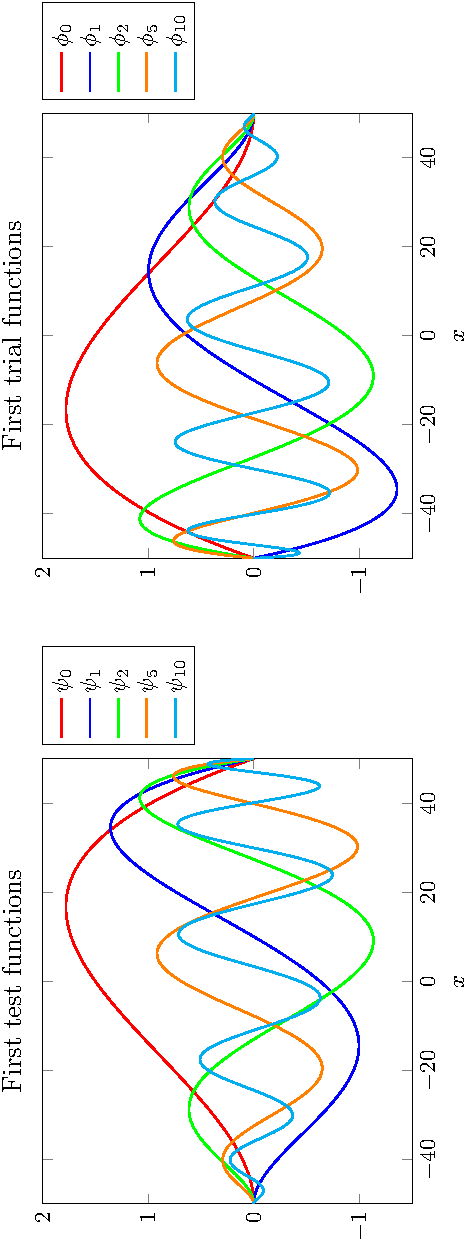
\includegraphics[scale=0.6,angle=270]{images/plotbasis2.pdf}
\caption{First test and trial functions.}
\label{basisfunctions}
\end{figure}
\end{center}


Thus for $N \geq 3$, we have
\beal
&V_N = \operatorname{span} \left\{ \phi_0,\phi_1,...,\phi_{N-3}\right\},\\
&V_N^{\ast} = \operatorname{span} \left\{ \psi_0,\psi_1,...,\psi_{N-3}\right\}.
\eeal
Then, we introduce the semi-discrete state variable $y_{N}(t,\cdot)$ on spectral space and its vector representation:
\be
y_N(t,\cdot) = \sum_{k=0}^{N-3}{\hat y_k(t)\phi_k(\cdot)},\quad \mathbf{y}(t) = \left( \hat y_0(t), \hat y_1(t), ..., \hat y_{N-3}(t)\right)^T.
\ee
The vector representation of the control is given by:
\be
\mathbf{u}(t) = \left( \langle u_{N}(t,\cdot), \psi_0(\cdot) \rangle, \langle u_{N}(t,\cdot), \psi_1(\cdot) \rangle, ..., \langle u_{N}(t,\cdot), \psi_{N-3}(\cdot) \rangle\right)^T
\label{discrcontrol}
\ee
where the form of the semi-discrete control $u_{N}(t,\cdot)$ is given in \cref{secdiscrcontrol}. Based on these discrete spaces, we build the matrices $M$, $P$, $Q$ and $S$ of size $(N-2)\times(N-2)$ with the coefficients $m_{ij}, p_{ij}, q_{ij}$ and $s_{ij}$ defined as follows:
\be
m_{ij}=(\phi_j, \psi_i),\quad p_{ij}=(\partial_x\phi_j, \psi_i),\quad q_{ij}=(\partial_x\phi_j, \partial_x\psi_i),\quad s_{ij}=(\partial_x\phi_j,\partial_{xx}\psi_i).
\label{definitionsmatrices}
\ee
The variational formulation \eqref{petrovgalerkin} thus yields
\be
M\frac{d\mathbf{y}}{dt} + \left(P +\gamma Q  + S \right)\mathbf{y} + F(\mathbf{y}) = \mathbf{u},
\ee
%<<<<<<< HEAD
%where $F(\mathbf{y})$ is the nonlinear term and is treated as suggested in \cite{shen2003new} i.e. using the pseudospectral approach. This means that the nonlinearity is evaluated in the spatial domain given by Chebyshev-Gauss-Lobatto (CGL) points, and is transferred back in the Legendre spectral space. Therefore, we need to be able to transform back and forth from the spectral space of Legendre coefficients to the values on the CGL points. This can be done using the fast Fourier transform (FFT) and the Chebyshev-Legendre transform. However, for the polynomial degrees we consider here (between 160 and 512), we use a simpler and more direct method which is faster and allows for an easier derivation of the discrete adjoint state equation (see \cref{numadjoint}). Beforehand we build the matrices  $L_1 =\left(\phi_j(x_i)\right)$ and $L_2 =\left(\psi_j(x_i)\right)$, $i=0 \ldots N$, $j=0 \ldots N-3$, where the points $x_i$ are the CGL points. By construction, those matrices satisfy
%=======
where $F(\mathbf{y})$ is the nonlinear term and is treated as suggested in \cite{shen2003new} i.e. using the pseudospectral approach. This means that the nonlinearity is evaluated in the spatial domain given by Chebyshev-Gauss-Lobatto (CGL) points, and is transferred back in the Legendre spectral space. Therefore, we need to be able to transform back and forth from the spectral space of Legendre coefficients to the values in the CGL points. This can be done using the fast Fourier transform (FFT) and the Chebyshev-Legendre transform. However, for the polynomial degrees we consider here (between 160 and 512), we use a simpler and more direct method which is faster and allows for an easier derivation of the discrete adjoint state equation (see \cref{numadjoint}).  {\color{red} It consists of building the matrices  $L_1 =\left(\phi_j(x_i)\right)$ and $L_2 =\left(\psi_j(x_i)\right)$, $i=0 \ldots N$, $j=0 \ldots N-3$ beforehand, where the points $x_i$ are the CGL points. By construction, those matrices satisfy
\be
L_1 \mathbf{y}(t) = \mathbf{\tilde{y}}(t) = (y_N(t, x_0), y_N(t, x_2), ...y_N(t, x_{N}))^T,
\label{spec2spat}
\ee
and the same holds true for a variable from $V_N^\ast$ with $L_2$. Thus the evaluation of the nonlinear term is given by
\be
L_1 F(\mathbf{y}(t)) = \mathbf{\tilde{y}}^2(t) = (y_N^2(t, x_0), y_N^2(t, x_2), ...y_N^2(t, x_{N}))^T.
\label{spec2spat2}
\ee}
Note that the spatial space, in which $\mathbf{\tilde{y}}(t)$ lies, and the spectral space, in which $\mathbf{y}(t)$ lies, do not have the same dimensions, i.e. $N+1$ versus $N-2$. This is only caused by the fact that the three boundary conditions are already included in the spectral space and not in the spatial space.
% \subsection{Time stepping scheme and adjoint - Crank-Nicolson}
% We have to deal with a problem of high order derivative. Therefore an explicit temporal discretization would lead to excessively small time steps in order to get stability. An implicit method should rather be considered. In \cite{li2000error}, the authors prove convergence of a pseudospectral method with backward Euler scheme for the \KdV equation. However in practice, the first order accuracy in time authorizes only very small time steps. A second order implicit scheme like the Crank-Nicolson scheme should be preferable, though the resolution of the nonlinear system is computationally demanding. This scheme also has the advantage of being a method of choice in optimal control: using the representation of the Crank-Nicolson scheme as a continuous Galerkin method of degree one (continuous trial linear functions and discontinuous piecewise constant test functions) allows us to give directly the concrete form of the adjoint, tangent and additional adjoint equations leading to the exact computation of the discrete gradient and Hessian \cite{meidner2007adaptive}. Note that the use of discrete derivatives is important for the convergence of our optimization algorithm. The scheme for the state is
%
% \bealn
% &M \tilde y_0=M y_0\\
% &M \tilde y_{n+1} + \frac{\Delta t}{2}\left( (S +\gamma Q -P)\tilde y_{n+1} - F(\tilde y_{n+1})\right)  &=  M \tilde y_{n} + \frac{\Delta t}{2}\left( (S +\gamma Q-P)\tilde y_{n} - F(\tilde y_{n})\right)  \\
%  &  &+ \frac{\Delta t}{2}\left( M\tilde q_n + M \tilde q_{n+1}\right), \quad n=0..N.
% \eealn
%
% Then the discrete adjoint scheme in case of distributed control writes
% %\begin{equation}\left\{
% %\begin{split}
% %M^t p_{N+1} + \frac{\Delta t}{2}\left( (S^t +\gamma Q^t- P^t)p_{N+1} - F'(y_{N+1})^t p_{N+1}\right) = -\frac{\Delta t}{2} A(y_{N+1} - y_d)\\
% % M^t p_{n-1} +  \frac{\Delta t}{2}\left( (S^t  +\gamma Q^t- P^t)p_{n-1}  - F'(y_{n-1})^t p_{n-1}\right)  &= M^t p_{n}\\
% %&- \frac{\Delta t}{2}A((y_{n} - y_d)-(y_{n-1} - y_d))+\frac{\Delta t}{2}\left( (S^t +\gamma Q^t- P^t)p_{n} - F'(y_{n-1})^t p_{n}\right) ,\\
% %&n=2..N+1
% %\end{split}
% %\right.
% %\end{equation}
% \bealn
% &M^t p_{N+1} + \frac{\Delta t}{2}\left( (S^t +\gamma Q^t- P^t)p_{N+1} - F^{'}(y_{N+1})^t p_{N+1}\right) = -\frac{\Delta t}{2} A(y_{N+1} - y_d) \\
% &M^t p_{n-1} +  \frac{\Delta t}{2}\left( (S^t  +\gamma Q^t- P^t)p_{n-1}  - F(y_{n-1})^t p_{n-1}\right)  = M^t p_{n} \\
% & \mbox{\hspace{0.15\textwidth}}- \frac{\Delta t}{2}A((y_{n} - y_d)-(y_{n-1} - y_d) + \frac{\Delta t}{2}\left( (S^t +\gamma Q^t- P^t)p_{n} - F^{'}(y_{n-1})^t p_{n}\right) ,\\
% & \mbox{\hspace{0.6\textwidth}}n=2..N+1\\
% &M^t p_{0}  = M^t p_{1} + \frac{\Delta t}{2}\left( (S^t +\gamma Q^t- P^t)p_{1} - F^{'}(y_{0})^t p_{1}\right)-\frac{\Delta t}{2} A(y_{1} - y_d)
% \eealn
% where the matrix $A = \left( \langle \phi_i,\phi_j\rangle\right)$ comes from the discretization of the Lagrangian (in particular the $L^2$ norm in the cost function). We also give the case of the terminal observations problem because we will use it in our numerical examples.
% \bealn
% & M^t p_{N+1} + \frac{\Delta t}{2}\left( (S^t +\gamma Q^t- P^t)p_{N+1} - F^{'}(y_{N+1})^t p_{N+1}\right) = - A(y_{N+1} - y_d)\\
% & M^t p_{n-1} + \frac{\Delta t}{2}\left( (S^t +\gamma Q^t- P^t)p_{n-1} - F^{'}(y_{n-1})^t p_{n-1}\right)  = M^t p_{n} + \\
% & \mbox{\hspace{0.35\textwidth}}\frac{\Delta t}{2}\left( (S^t +\gamma Q^t- P^t)p_{n} - F^{'}(y_{n-1})^t p_{n}\right), \, n=2..N+1\\
% &M^t p_{0}  = M^t p_{1} + \frac{\Delta t}{2}\left( (S^t +\gamma Q^t- P^t)p_{1} - F^{'}(y_{0})^t p_{1}\right)
%  \eealn

\subsubsection{Semi-discretization of the control $u$}
\label{secdiscrcontrol}
By $\left\{x_i \right\}, i = 0, 1, \ldots, N$, we denote the grid points of the spatial mesh (i.e. in our case the CGL points). The control is then discretized as follows
\be
u_N(t, \cdot) = \sum_{j=0}^{N}{\hat u_j(t)\delta_{x_j}(\cdot)}
\ee
where $\delta_{x_j}$ are Dirac functionals located at the grid points $x_j$ and the functions $\hat u_j(t)$ are its time-dependent coefficients. Hence, there holds $u_N \in \M$. Thus the righthand side of \eqref{petrovgalerkin} takes the form
\be
\langle u_N(t),\psi\rangle = \sum_{j=0}^{N}{\hat u_j(t)\psi(x_j)}.
\label{discrpscontrol}
\ee
Moreover we introduce another vectorized representation of the variable $u_{N}$
\be
\mathbf{\hat u}(t) = \left( \hat u_{0}(t), \ldots, \hat u_{N}(t)\right)^{T}.
\label{discrcontrolindirac}
\ee
This representation of the discrete control will be useful in the definition of the various norms involved in the optimization process.
%as well as the norm in the objective functional
%\be
%\|{u_N}\|_{\M} = \sum_{j=1}^N{\left( \sum_{i = 1}^{N_T}{\tau_i u_{ji}^2}\right)^{1/2}},
%\ee
%where $N_T$ is the number of time steps and $\tau_i$ is the size of the $i^{th}$ step. We point out that this precise control discretization was also used and analyzed in \cite{pieper2013priori, pieper2014,casas2013parabolic}.

\subsubsection{Time stepping scheme and adjoint - Crank-Nicolson-Leap-Frog}
\label{numadjoint}
The \KdVB equation involves a high order derivative. Therefore an explicit temporal discretization would lead to small time steps in order to get stability. Thus an implicit method seems to be more more appropriate. In \cite{li2000error}, the authors prove convergence of a pseudospectral method in space combined with a backward Euler scheme for the \KdV equation. Due the first order convergence of this method, small time steps are required to achieve a good level of accuracy. Therefore, a second order implicit scheme like the Crank-Nicolson scheme is preferable. This scheme is well studied in the context of optimal control of PDEs. Using the representation of the Crank-Nicolson scheme as a Petrov-Galerkin method with continuous linear trial functions and discontinuous piecewise constant test functions determines the form of the discrete adjoint, tangent and additional adjoint equations. The solutions of these discrete equations are used for the exact computation of the discrete gradient and Hessian, e.g. \cite{meidner2007adaptive}. Note that the use of the exact discrete derivatives is important for the convergence of optimization algorithms. However, the Crank-Nicolson scheme is computationally demanding. An alternative is the two-step Crank-Nicolson-Leap-Frog (CNLF) method in which the third derivative is treated implicitly and the nonlinear term is treated explicitly. This method has already been extensively used for the \KdV equation, cf. \cite{shen2003new,ma2000legendre,ma2001optimal}.
%showing for instance extended stability intervals with the Fourier spectral method \cite{chan1985fourier}. However, to the authors' knowledge, this has never been used in the context of an optimal control problem.
Commonly, it is initialized by a semi-implicit step. We suggest also a slight modification of the last step of this two-step method in order to get a discrete adjoint state equation that is consistent with the continuous adjoint state equation.\\
The time domain is divided into $N_{T}$ intervals, i.e. $0 = t_0 < t_1....< t_{N_{T}} = T$. The first and last one have length $\frac{\Delta t}{2}$ and the other steps are of equal length $\Delta t$. The fully discrete state variable has the form
$$\mathbf{y}_n = \mathbf{y}(t_n) = \left( \hat y_0(t_n), \hat y_1(t_n), ..., \hat y_{N-3}(t_n)\right)^T,  \quad  n=0 \ldots N_{T}$$ and the control
\beal
&\mathbf{u}_n = \mathbf{u}(t_n) = \left( \langle u_{N}(t_n,\cdot), \psi_0(\cdot) \rangle, \langle u_{N}(t_n, \cdot), \psi_1(\cdot) \rangle, ..., \langle u_{N}(t_n, \cdot), \psi_{N-3}(\cdot) \rangle\right)^T, \\
&\mathbf{\hat u}_n = \mathbf{\hat u}(t_n) = \left( \hat u_{0}(t_{n}), \ldots, \hat u_{N}(t_{n})\right)^{T}, \quad  n=0 \ldots N_{T}
\eeal
where the duality pairing $\langle\cdot,\cdot\rangle$ is evaluated according to \eqref{discrpscontrol}. With the help of the matrices defined in \eqref{definitionsmatrices}, the forward scheme looks as follows
\bealn\label{forwardscheme}
& \frac{1}{2}\left( M+\Delta t S\right) \mathbf{y}_1 = \frac{1}{2}\left( M + \Delta t \left(P + \gamma  Q \right) \right) \mathbf{y}_0 + \frac{1}{2}\Delta t F(\mathbf{y}_0) + \frac{1}{2}\Delta t \mathbf{u}_0 \\
& \frac{1}{2}\left( M+\Delta t S\right) \mathbf{y}_{n+1} = \frac{1}{2}\left( M - \Delta t S\right) \mathbf{y}_{n-1} +  \Delta t \left( P + \gamma Q\right)\mathbf{y}_n \\
& \mbox{\hspace{0.5\textwidth}}+ \Delta t F(\mathbf{y}_n) + \Delta t \mathbf{u}_n,  \, n=1 \ldots N_{T}-1\\
& M \mathbf{y}_{N_{T}+1} = \frac{1}{2}\left( M \mathbf{y}_{N_{T}} + M \mathbf{y}_{N_{T}-1} \right)+ \frac{1}{2}\Delta t \left(P + \gamma Q \right)\mathbf{y}_{N_{T}} \\
& \mbox{\hspace{0.5\textwidth}} + \frac{1}{2}\Delta t F(\mathbf{y}_{N_{T}}) - \frac{1}{2}\Delta t S \mathbf{y}_{N_{T}-1}
\eealn
The first step is semi-implicit. The steps $n=1 \ldots N_{T}-1$ are classical CNLF steps. The last step is not a regular step. It is designed in a way such that the discrete adjoint state equation is consistent with a CNLF discretization of the continuous adjoint state equation. Notice, that this step becomes the mean value between the two preceding steps for $\Delta t\downarrow0$.
The corresponding discrete objective functional has the form
\begin{multline}
J_{N,N_{T}}(\mathbf{y}_{0}, \ldots, \mathbf{y}_{N_{T}}, \mathbf{u}_{0}, \ldots, \mathbf{u}_{N_{T}}) = \frac{1}{2}\sum_{i=1}^{N_{T}}{\Delta t \left(\mathbf{y}_{i} - \mathbf{z}_{1,i}\right)^{t}A \left(\mathbf{y}_{i} - \mathbf{z}_{1,i}\right)} + \\ \frac{1}{2}\left(\mathbf{y}_{N_T} - \mathbf{z}_{2}\right)^{t}A \left(\mathbf{y}_{N_T} - \mathbf{z}_{2}\right)
 + \alpha \sum_{j=1}^N{\left( \sum_{i = 1}^{N_T}{\Delta t \mathbf{\hat u}_{ij}^2}\right)^{1/2}}
\label{discrobj}
\end{multline}
where entries of $A$ are given by $a_{ij}=(\chi_{\Omega_o}\phi_j, \psi_i)_{L^2(\Omega)}$.
Then we define the discrete Lagrangian function:
\begin{multline}
\mathcal{L}_{N,N_{T}}(\mathbf{y}_{0}, \ldots, \mathbf{y}_{N_{T}},\mathbf{u}_{0}, \ldots, \mathbf{ u}_{N_{T}}, \mathbf{p}_{0}, \ldots, \mathbf{p}_{N_{T}-1}) = \\
J_{N,N_{T}}(\mathbf{y}_{0}, \ldots, \mathbf{y}_{N_{T}}, \mathbf{u}_{0}, \ldots, \mathbf{u}_{N_{T}})  +\\
\mathbf{p}_0^T\left[ \frac{1}{2}\left( M+\Delta t S\right) \mathbf{y}_1 - \frac{1}{2}\left( M + \Delta t P + \gamma \Delta t Q \right) \mathbf{y}_0 - \frac{1}{2}\Delta t F(\mathbf{y}_0) - \frac{1}{2}\Delta t \mathbf{u}_0 \right]+\\
\sum_{k=1}^{N_T-2}{\mathbf{p}_k^T\left[\frac{1}{2}\left( M+\Delta t S\right) \mathbf{y}_{k+1} - \frac{1}{2}\left( M - \Delta t S\right) \mathbf{y}_{k-1} - \Delta t \left( P + \gamma Q\right)y_k \right.}\\
\left.- \Delta t F(y_k) - \Delta t \mathbf{u}_k\right] + \\
\mathbf{p}_{N_T-1}^T\left[ M \mathbf{y}_{N_T} - \frac{1}{2}\left( M \mathbf{y}_{N_T-1} + M \mathbf{y}_{N_T-2} \right)- \frac{1}{2}\Delta t \left(P+ \gamma Q\right) \mathbf{y}_{N_T - 1} \right.\\ \left.- \frac{1}{2}\Delta t F(\mathbf{y}_{N_T-1}) +\frac{1}{2}\Delta t S \mathbf{y}_{N_T-2}\right].
\label{discrlag}
\end{multline}
From \eqref{discrlag}, we can derive the discrete adjoint state equation which has the form
 \bealn
 &M^T \mathbf{p}_{N_T-1} = -A(\mathbf{y}_{N_T} - \mathbf{z}_2)\\
 &\frac{1}{2}\left( M^T+\Delta t S^T\right) \mathbf{p}_{N_T-2} = \frac{1}{2}\left( M^T + \Delta t P^T + \gamma \Delta t Q^T \right) \mathbf{p}_{N_T - 1} \\
 &\mbox{\hspace{0.3\textwidth}} + \frac{1}{2}\Delta t F^{'}(\mathbf{y}_{N_T - 1})^T \mathbf{p}_{N_T - 1} \\
 &\frac{1}{2}\left( M^T + \Delta t S^T\right)\mathbf{p}_{n-2} = \frac{1}{2}\left( M^T - \Delta t S^T\right)\mathbf{p}_{n} + \Delta t \left( P^T + \gamma Q^T\right)\mathbf{p}_{n-1} \\
 &\mbox{\hspace{0.3\textwidth}}+ \Delta t F^{'}(\mathbf{y}_{n-1})^T \mathbf{p}_{n-1},\quad n=2 \ldots N_T - 1.
 \label{numschemeadj}
\eealn
in the case of terminal observations, which will be of particular interest in the numerical examples. In the first equation the terminal value of the discrete adjoint state is set. This is followed by a single semi-implicit step and regular CNLF steps.
% The lagrangian of the problem writes at the continuous level.
% \beal
%   \mathcal{L}(y,q,p) = \frac{1}{2}\norm{y - y_d}_{\lspace}^2 + \alpha \norm{q}_{\M} + <p, By-q>
% \eeal
% Its (almost) discrete counterpart shall be
% \begin{multline}
% L(\bar y, \bar q, \bar p) = \frac{1}{2}(y_{N+1} - y_d)^t A (y_{N+1} - y_d) + \alpha \norm{q}_{\M} \\
% + p_0^t\left[ \frac{1}{2}\left( M+\Delta t S\right) y_1 - \frac{1}{2}\left( M + \Delta t P + \gamma \Delta t Q \right) y_0 - \frac{1}{2}\Delta t F(y_0) - \frac{1}{2}\Delta t M q_0 \right]\\
% +\sum_{k=1}^{N-1}{p_k^t\left[
% \frac{1}{2}\left( M+\Delta t S\right) y_{k+1} - \frac{1}{2}\left( M - \Delta t S\right) y_{k-1} - \Delta t \left( P + \gamma Q\right)y_k - \Delta t F(y_k) - \Delta t M q_k\right]}\\
% +p_N^t\left[ M y_{N+1} - \frac{1}{2}\left( M y_N + M y_{N-1} \right)- \frac{1}{2}\Delta t P y_N - \frac{1}{2}\Delta t F(y_N) +\frac{1}{2}\Delta t S y_{N-1}\right].
% \end{multline}
% Differentiating with respect to $\bar y$ leads
% \begin{multline}
% \delta L(\bar y, \bar q, \bar p)\delta \bar y = \delta y_{N+1}^t A (\delta y_{N+1} - y_d) \\
% + p_0^t\left[ \frac{1}{2}\left( M+\Delta t S\right) \delta y_1 - \frac{1}{2}\left( M + \Delta t P + \gamma \Delta t Q \right) \delta y_0 - \frac{1}{2}\Delta t F'(y_0)\delta y_0\right]\\
% +\sum_{k=1}^{N-1}{p_k^t\left[
% \frac{1}{2}\left( M+\Delta t S\right) \delta y_{k+1} - \frac{1}{2}\left( M - \Delta t S\right) \delta y_{k-1} - \Delta t \left( P + \gamma Q\right)y_k - \Delta t F'(y_k)\delta y_k \right]}\\
% +p_N^t\left[ M \delta y_{N+1} - \frac{1}{2}\left( M \delta y_N + M \delta y_{N-1} \right)- \frac{1}{2}\Delta t P \delta y_N - \frac{1}{2}\Delta t F'(y_N)\delta y_N + \frac{1}{2}\Delta tS\delta y_{N-1}\right]
% \end{multline}
% Symmetry of the scalar product yields, after re-indexing of the terms
% \beal
% \delta L(\bar y, \bar q, \bar p)\delta \bar y &= \delta y_{N+1}^t A (\delta y_{N+1} - y_d) \\
% &+ \left[ \delta y_1^t\frac{1}{2}\left( M+\Delta t S\right)  - \delta y_0^t\frac{1}{2} \left( M + \Delta t P + \gamma \Delta t Q \right) - \delta y_0^t\frac{1}{2}\Delta t F^{'}(y_0)\right]p_0\\
% &+\sum_{k=2}^{N}{\delta y_k^t\left[
% \frac{1}{2}\left( M+\Delta t S\right)^t \right]p_{k-1}}-\sum_{k=0}^{N-2}{\delta y_k^t\left[\frac{1}{2}\left( M+\Delta t S\right)^t \right]p_{k+1}}\\
% &-\sum_{k=1}^{N-1}{\left[ \delta y_k^t \Delta t\left(P^t + \gamma Q^t + F^{'}(y_k)^t\right)\right]p_k}\\
% &+\delta y_{N+1}^t M^t p_N - \delta y_{N-1}^t \frac{1}{2}(M^t - \Delta t S^t)p_N \\
% &-\delta y_{N}^t \left( \frac{1}{2}(M^t + \Delta t P^t + \Delta t F^{'}(y_N)^t) \right)p_N.
% \eeal
% The discrete adjoint scheme is obtained by imposing $\delta L(\bar y, \bar q, \bar p)\delta \bar y = 0$.
\begin{remark}
Without this modification of the last step in \eqref{forwardscheme}, the discrete adjoint state equation obtained in the case of terminal observation would be
\bealn
&\frac{1}{2}(M^T+\Delta t S^T) \mathbf{p}_{N_T-1} = -A(\mathbf{y}_{N_T} - \mathbf{z}_2)\\
&\frac{1}{2}\left( M^T+\Delta t S^T\right) \mathbf{p}_{N_T-2} =  \left(\Delta t P^T + \gamma \Delta t Q^T \right) \mathbf{p}_{N_T-1} + \Delta t F^{'}(\mathbf{y}_{N_T - 1})^T \mathbf{p}_{N_T - 1} \\
&\frac{1}{2}\left( M^T + \Delta t S^T\right)\mathbf{p}_{n-2} = \frac{1}{2}\left( M^T - \Delta t S^T\right)\mathbf{p}_{n} + \Delta t \left( P^T + \gamma Q^T\right)\mathbf{p}_{n-1} \\
&\mbox{\hspace{0.4\textwidth}}+ \Delta t F^{'}(\mathbf{y}_{n-1})^T \mathbf{p}_{n-1}, \quad n=2 \ldots N_T-1.
\eealn
The major difference is the second step. It does not correspond to a consistent discretization of the continuous adjoint state equation. The time derivative is not reconstructed. In practice this would result in large oscillations in time of the adjoint variable.
\end{remark}
\begin{remark}
Unlike the other steps, the modified last step in \eqref{forwardscheme} involves the inversion of the matrix $M$, which is typically ill-conditioned. Therefore, we invert the matrix $M+\varepsilon Id$ with a $\varepsilon$ of the order $h^2$, where $h$ is the largest space step.
\end{remark}
\begin{proposition}
The directional derivative of
\[
\{\mathbf u_i\}_{i=1}^{N_T}\mapsto\frac{1}{2}\left(\mathbf{y}_{N_T} - \mathbf{z}_{2}\right)^{t}A \left(\mathbf{y}_{N_T} - \mathbf{z}_{2}\right),
\]
where $\{\mathbf y_i\}_{i=1}^{N_T}$ is the solution of \eqref{forwardscheme}, is given by $\{-\mathbf{p}_i\}_{i=1}^{N_T}$, where $\{\mathbf{p}_i\}_{i=1}^{N_T}$ is the solution of \eqref{numschemeadj}.
\end{proposition}
\begin{proof}
The proof is done by standard differentiation of the discrete Lagrangian.
\qquad\end{proof}

\subsection{Numerical treatment of the optimization problem}
{\color{red} In this section we consider the optimal control problem \eqref{cost} in both the viscous and non-viscous case, i.e. $\gamma\geq0$, without additional norm-constraints on the control. Thus we have $U_{ad}=\M$.}
\subsubsection{The regularized problem}
In this section, we discuss the solution of the optimal control problem \eqref{cost} by Newton type method and a continuation strategy. We introduce an additional $L^2$ regularization term in \eqref{cost}:
\begin{multline}
\min_{u \in L^2(\Omega_c\times I), y\in Y}J(y,u)=\frac{1}{2}\left(\norm{\chi_{\Omega_{o}}y - z_1}_{L^2(I\times \Omega_{o})}^2+\|\chi_{\Omega_{o}}y(T)-z_2\|_{L^2(\Omega_{o})}^2\right)\\
+\alpha \norm{u}_{L^1(\Omega_c, L^{2}(I))} + \frac{\rg}{2}\norm{u}_{L^2(I\times\Omega_c)}^2\quad\text{s.t.}~\eqref{kdvcontrol1}-\eqref{kdvcontrol3}.
\label{costreg}
\end{multline}
%\beal
%\min_{u \in \M} J(y) &= \frac{1}{2}\norm{y - y_d}_{\lspace}^2 + \alpha \norm{u}_{L^1(\Omega,L^2(I))} + \frac{\rg}{2}\norm{u}_{L^2(\Omega,L^2(I))}^2 \\
%& = f(y) + \alpha \norm{u}_{L^1(\Omega,L^2(I))} + \frac{\rg}{2}\norm{u}_{L^2(\Omega,L^2(I))}^2,
%\label{costreg}
%\eeal
This problem is posed in the Hilbert space $L^2(I\times\Omega_c)$. Since the embedding $L^1(\Omega_c,L^2(I))\hookrightarrow \M$ is isometric, we have
\be
\psi(u) = \norm{u}_{\M} = \norm{u}_{L^1(I,L^2(\Omega_c))} = \int_{\Omega_c}{\norm{u(x)}_{L^2(I)}dx}.
\ee
for any $L^2(I\times \Omega_c)$. In \cite{herzog2012directional}, the authors study this problem in the linear parabolic case, and prove that this setting promotes a \textit{striped sparsity pattern} of the optimal control. For the derivation of optimality conditions, we introduce the proximal map of the $L^1(\Omega_c, L^{2}(I))$ norm, e.g. \cite{bauschke2011convex}:
\be
\operatorname{Prox}_{\psi/ \rg}(q)(t,x) = \left(1-\frac{\alpha}{\rg\norm{q(x)}_{L^{2}(I)}}\right)^{+}q(t,x) \quad \mbox{ for } q \in L^{2}(I\times\Omega_c).
\ee
We can then express the optimality condition for \eqref{costreg} by the pointwise formula
\be
\bar u_{\rg}(t,x) = \operatorname{Prox}_{\psi/ \rg}\left(-\frac 1\rg \bar p_\rg\right)(t,x)=-\frac{1}{\rg}\left( 1 - \frac{\alpha}{\norm{\bar p_{\rg}(x)}_{L^{2}(I)}}\right)^{+}\bar p_{\rg}(t,x)
\ee
where $\bar p_\rg$ solves \eqref{adjointKdV1}-\eqref{adjointKdV3} for $\phi=\bar y_\rg-z_1$, $y=\bar y_\rg$ and $p_T=\bar y_\rg(T)-z_2$ and $\bar y_\rg$ solves \eqref{kdvcontrol1}-\eqref{kdvcontrol3} for $\bar u$. Now a Newton type method can applied for the solution of
\be
F(u_{\rg})(t,x) = \rg u_{\rg}(t,x) + \left( 1 - \frac{\alpha}{\norm{p_{\rg}(x)}_{L^{2}(I)}}\right)^{+}p_{\rg}(t,x) = 0.
\label{optcondition}
\ee
However, we follow \cite{pieperthesis} and reformulate the optimality condition \eqref{optcondition} using the "normal map" due to Robinson and solve instead  
\be
\operatorname{G}(q_{\rg}) = \rg q_{\rg} + p_{\rg}(y_\rg(\operatorname{Prox}_{\psi/ \rg}(q_{\rg}))) = 0,
\label{normalmap}
\ee
for the auxiliary variable $q_{\rg}$. Here $p_\rg$ solves \eqref{adjointKdV1}-\eqref{adjointKdV3} for $\phi=y_\rg-z_1$, $y=y_\rg$ and $p_T=y_\rg(T)-z_2$ and $y_\rg$ solves \eqref{kdvcontrol1}-\eqref{kdvcontrol3} for $u=\operatorname{Prox}_{\psi/ \rg}(q_{\rg})$.  %such that $u_{\rg} = \operatorname{Prox}_{\psi/ \rg}(q_{\rg})$ h. %One easily prove in that case that $q_{\rg} = -\frac{1}{\rg} p_{\rg}$ and equivalence between \eqref{optcondition} and \eqref{normalmap}.

% and we can adapt it to state the following theorem
% \begin{thm}
%  Let $\gamma > 0$. Problem \eqref{costreg} possesses a unique optimal solution  $q_{\gamma} \in L^2(I\times\Omega)$ with corresponding state $y_{\gamma} = S(y_0,q_{\gamma})$ and adjoint state $p_{\gamma} = S'^{\ast}(y_{\epsilon} - y_d)$. The first order optimality condition is the subgradient condition
%  \be
%  -<q - q_{\gamma}, \frac{1}{\gamma}q_{\gamma} + p_{\gamma}> +\alpha \norm{q_{\gamma}}_{L^1(I,L^2(\Omega))} \leq \alpha \norm{q}_{L^1(I,L^2(\Omega))}
%  \ee
%  for all $q \in L^1(I,L^2(\Omega))$. This is summed up in the formula
%  \be
%  u_{\gamma}(t,x) = \gamma\max\left(0,1-\frac{\alpha}{\norm{p_{\gamma}}_{L^2(I)}}\right)p_{\gamma}(t,x)
%  \ee
%  for almost all $(t,x)\in I\times\Omega$.
% \end{thm}
% The idea is then to solve with a semismooth Newton method \cite{ulbrich2002semismooth} the equation
% \be
% F(q_{\gamma}) = q_{\gamma} - \gamma\max\left(0,1-\frac{\alpha}{\norm{p_{\gamma}}_{L^2(I)}}\right)p_{\gamma}(t,x)
% \ee
% In comparison to what is done in \cite{herzog2012directional}, the nonlinearity in our problem requires that we additionally compute the tangent and the second adjoint operators to get the gradient of $F$. Besides, in \cite{pieper2014}, the authors quickly prove that we obtain the original problem in the limiting case for great $\gamma$.
For the solution of problem \eqref{normalmap}, we apply a Newton-type method, and since the proximal operator is not differentiable, we use the concept of semismoothness to derive a generalized derivative for $\operatorname{G}$, cf. \cite{ulbrich2002semismooth}. {\color{red}To be more precise, we have
\be
\operatorname{DG}(q_{\rg})\delta q = \rg\delta q + \delta p(\delta y(\operatorname{DProx}_{\psi/ \rg}(q_{\rg})\delta q)),\quad \delta q\in L^2(I\times \Omega_c),
\ee
where $\delta p$ solves the equation \eqref{adjointKdV1}-\eqref{adjointKdV3} for $\phi=\delta y(1+\partial_y p_\rg)$, $y=y_\rg$ and $p_T=\delta y(T)$ and $\delta y$ solves \eqref{linearizedkdv1}-\eqref{linearizedkdv3} 
for $\delta u=\operatorname{DProx}_{\psi/ \rg}(q_{\rg})\delta q$ and $y=y_\rg$. The generalized derivative of the proximal map is given by
\begin{numcases}{\operatorname{DProx}_{\psi/ \rg}(q_{\rg})\delta q = }
\left(1-\frac{\alpha}{\rg\norm{q_{\rg}}_{L^{2}(I)}}\right)\delta q + \frac\alpha\rg \frac{\left( q_{\rg}, \delta q\right)_{L^2(I)}}{\norm{q_{\rg}}_{L^{2}(I)}^3}q_{\rg} & \nonumber \\
 & \hspace{-1.5cm} \mbox{if   $\norm{q_{\rg}}_{L^{2}(I)} > \frac{\alpha}{\rg} $}\nonumber\\
0 & \mbox{otherwise.}
\end{numcases}}
The great advantage of the normal map approach is that the Newton operator $DG(q_{\rg})$ is symmetric with respect to the scalar product $(\cdot,\operatorname{DProx}_{\psi/ \rg}(q_{\rg})\cdot)_{L^2(I\times\Omega_c)}$, cf. \cite{PieperRund2015,pieperthesis}. Therefore the conjugate gradient method can be used to solve the Newton system. The operator $DF(u_\rg)$ is in general not symmetric. In the case of a linear state equation numerical experiments show that the continuation strategy in $\rg$ is sufficient to achieve global convergence, e.g. \cite{ClasonKunisch:2011b}. This is not the case for our problem due to the nonlinearity of the state equation. Additional to the continuation strategy in $\rg$ a globalization strategy based on the decrease of the regularized objective functional is required. We implement a trust region semi-smooth Newton based on the truncated conjugate gradient algorithm by Steihaug \cite{pieperthesis,steihaug1983}. {\color{red}A concise explanation is also available in \cite[Section 6.2 and A.3]{PieperRund2015}}.

\subsubsection{Discretization of the control and mass lumping}
In the unregularized problem, the controls are discretized as nodal Dirac measures. In the regularized case, this is not possible due to $L^2(I\times\Omega_c)$ regularization term. Thus we introduce a discretization of the control which is compatible to the Dirac discretization in the limiting case $\rg \to 0$, i.e. we follow the strategy in \cite{pieper2014}. The control is discretized in space with piecewise linear and continuous finite elements on a grid whose nodes are given by the CGL-points $(x_n)$, $n=0 \ldots N$ previously mentioned.
% The finite element space associated with this grid is
% \be
% V_h = \left\{ u_h \in \mathcal{C}_0 (\Omega) \,|\, u_{h|K} \in \mathcal{P}_1(K) \mbox{ for all } K \in \mathcal{T}_h \mbox{ and } u_{h|\partial \Omega} = 0 \right\}.
% \ee
% The discretization parameter h denotes the maximum length of the intervals defined by the CGL points. For the time discretization, we define for any Banach space $V$ the semi-discrete space
% \be
% X_\tau^0 (I,V) = \left\{ v_{\tau} \in L^2(I,V) \, | \, v_{\tau|I_m} \in P_0(I_m,V), m=1..N_T\right\},
% \ee
% where $I_m = (t_{m-1}, t_m]$ and $0 = t_0 < t_1....< t_m = T$. The time steps are denoted $\tau_m = t_m - t_{m-1}$ and by $\tau$ we designate the maximum of them. The full discrete space for the control is then $X_{\tau}^0(I,V_h)$.
Thus, the discrete control has the form
\[
u_h = \sum_{j=1}^{N_T}{\chi_{I_j}\sum_{n=0}^{N}{\mathbf{\hat u}_{jn} e_n}},
\]
where $\chi_{I_j}$, $I_{j} = (t_{j-1}, t_j]$ is the characteristic function of the $j^{th}$ time interval, and $e_{n}$ is the finite element basis function centered at the grid point $x_{n}$. All scalar products and norms involving the discrete control are computed using mass lumping, i.e. the trapezoidal rule is used for the evaluation of the spatial integrals on each cell. Therefore, we have
\beal
&\norm{u_h}_{L^1(\Omega, L^2(I))} = \sum_{n=0}^N{d_n\left(\sum_{j=1}^{N_T}{\Delta t \mathbf{\hat u}_{nj}^2}\right)^{1/2}}, \quad \norm{u_h}_{L^2(\Omega, L^2(I))}^2 = \sum_{n=0}^N{d_n\left(\sum_{j=1}^{N_T}{\Delta t \mathbf{\hat u}_{nj}^2}\right)},\\
&\langle u_h,\psi \rangle_{L^2(\Omega)} = \sum_{j=1}^{N_T} \chi_{I_j} \sum_{n=0}^N{d_n \mathbf{\hat u}_{jn}\psi_{n}}
\label{masslumping}
\eeal
for all spectral basis functions $\psi$ where $\psi_n = \psi(x_n)$ and $d_n = \int_{\Omega_c}{e_n~\mathrm{d}x}$.
%$\varphi_h = \sum_{j=1}^{N_T}{\chi_{I_j}\sum_n{\varphi_{jn} e_n}}$.

\begin{remark}
Due to the use of \eqref{masslumping}, the formulas \eqref{optcondition} resp. \eqref{normalmap} hold also on the discrete level.
\end{remark}


\subsection{Numerical examples}\label{num_ex}
In this section, we investigate an inverse problem involving the flow of water in a narrow channel and the problem of the optimal positioning and vertical movement of a wavemaker. A similar optimal design problem is carried out in \cite{nersisyan2014generation}. A possible application is the design of artificial surfing facilities. For that purpose, we use a version of the forced \KdV equation with physical motivated parameters, as in \cite{milewski2004forced}:
\be
\partial_t y + f \partial_x y - \frac{1}{6}\partial_{xxx} y - \frac{3}{2}y \partial_x y = u
\label{PhysicalKDV}
\ee
where the parameter $f$ is proportional to $F-1$ ($F$ is the Froude number). Its value determines if a flow is subcritical ($f\leq 0$) or supercritical ($f> 0 $). The forcing $u$ is interpreted as the spatial derivative of the bottom topography of the channel. In both examples, we consider the minimization problem
\be
\min_{u \in \mathcal{M}(\Omega_c,L^2(I)), y\in Y}J(y,u) =\frac{1}{2}\|\chi_{\Omega_{o}}y(T)-z\|_{L^2(\Omega_{o})}^2 +\alpha \norm{u}_{\mathcal{M}(\Omega_c, L^{2}(I))}
\ee
for different $\Omega_c$, $\Omega_o$ and $z$, where $y$ is the solution of \eqref{PhysicalKDV}. In particular, we emphasize that $U_{ad} = \mathcal{M}(\Omega_c,L^2(I))$ and $\gamma=0$. In all numerical examples, we have never encountered blow ups of $y$.

\paragraph{\underline{Inverse problem}}
In the first example, we reconstruct the time-varying bottom topography which creates water waves in a narrow channel. These waves are observed at final time T. We generate beforehand a wave with the following source term
\begin{numcases}
{u^\dag(t,x) = }
 \nonumber 10\delta_{\{x = 1.5\}}, \mbox{ when } 0 < t\leq 2.5 \\
 0, \mbox{ when } 2.5 \leq t\leq 5
 \label{forcingq}
\end{numcases}
in a subcritical configuration ($f = -0.5$). The time horizon is $T = 5$. The space-time grid is parametrized with $N = 256$ spatial grid points and a time-step size of $\Delta t = 0.01$. The generated wave is displayed in \cref{waveobservation}.
\begin{figure}[htb]
\subfloat{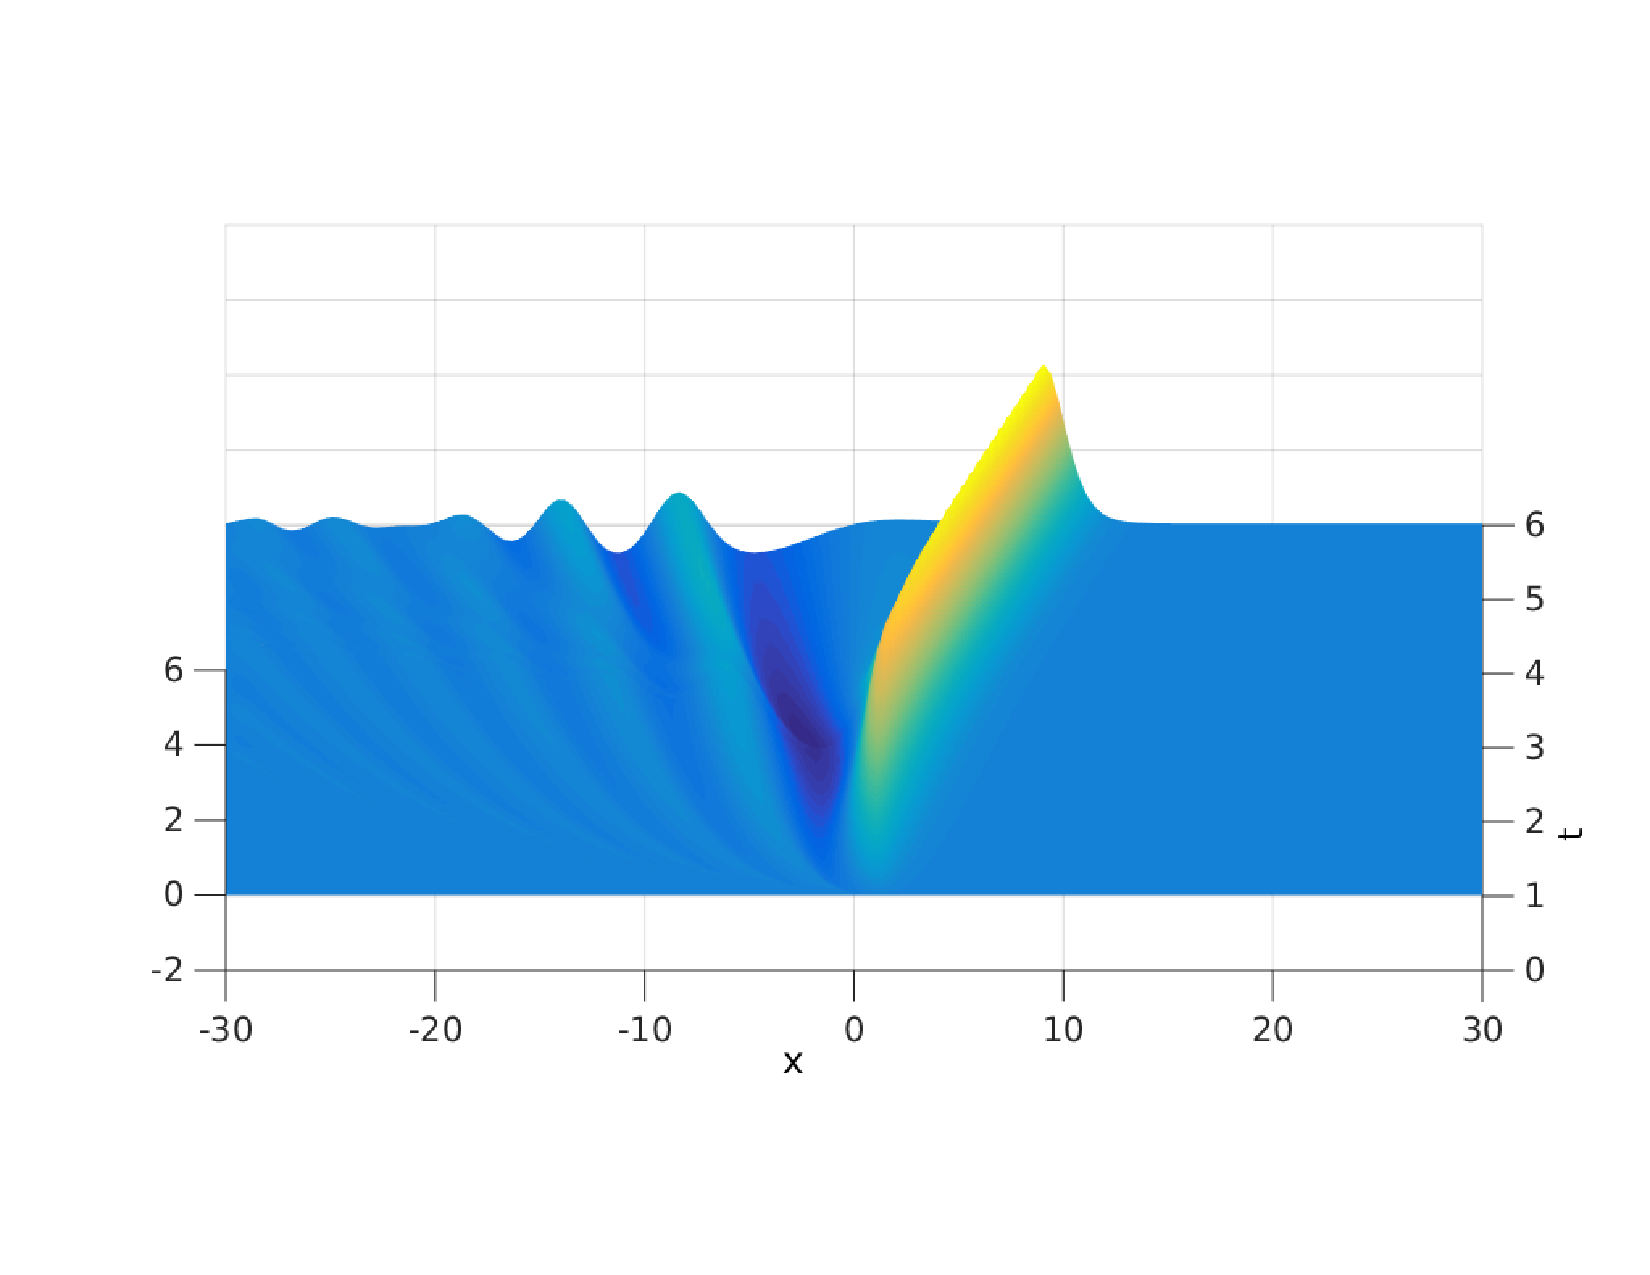
\includegraphics[width=0.48\textwidth]{images/ex1yd3D.pdf}}\quad
\subfloat{% This file was created by matlab2tikz.
% Minimal pgfplots version: 1.3
%
%The latest updates can be retrieved from
%  http://www.mathworks.com/matlabcentral/fileexchange/22022-matlab2tikz
%where you can also make suggestions and rate matlab2tikz.
%
\definecolor{mycolor1}{rgb}{0.00000,0.44700,0.74100}%
%
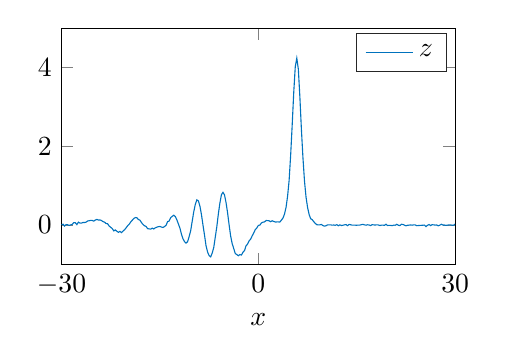
\begin{tikzpicture}

\begin{axis}[%
width=5cm,
height=3cm,
at={(0.0in,0.0in)},
scale only axis,
xmin=-30,
xmax=30,
xtick={-30,0,30},
xlabel={$x$},
ymin=-1,
ymax=5,
legend style={legend cell align=left,align=left,draw=white!15!black}
]
\addplot [color=mycolor1,solid]
  table[row sep=crcr]{%
-30	0.00669380296960023\\
-29.765625	0.0231418779869073\\
-29.53125	-0.0270253165049322\\
-29.296875	0.0133492509621372\\
-29.0625	0.00846191891086888\\
-28.828125	-0.0090641890303429\\
-28.59375	0.00482433352954454\\
-28.359375	0.0184656700659997\\
-28.125	0.0629589092184118\\
-27.890625	0.0582123649530002\\
-27.65625	0.0124276962484976\\
-27.421875	0.0737487737669349\\
-27.1875	0.0517707366756799\\
-26.953125	0.0499621122217574\\
-26.71875	0.0674258613489597\\
-26.484375	0.0648477220299364\\
-26.25	0.0741371987358284\\
-26.015625	0.103376744333651\\
-25.78125	0.110509351859353\\
-25.546875	0.119192090962731\\
-25.3125	0.11685728966342\\
-25.078125	0.100181851515093\\
-24.84375	0.128553063638925\\
-24.609375	0.143114863219125\\
-24.375	0.128238796853503\\
-24.140625	0.130360438642391\\
-23.90625	0.115543164891435\\
-23.671875	0.0868408606915378\\
-23.4375	0.0748963683042355\\
-23.203125	0.0385688968660524\\
-22.96875	0.0331593366129867\\
-22.734375	-0.0254997138237426\\
-22.5	-0.0561915697866013\\
-22.265625	-0.0894599613955862\\
-22.03125	-0.148712021045533\\
-21.796875	-0.123568700737615\\
-21.5625	-0.157702304339356\\
-21.328125	-0.184769341003744\\
-21.09375	-0.160983049853647\\
-20.859375	-0.190718047208251\\
-20.625	-0.151487168391879\\
-20.390625	-0.119092254074365\\
-20.15625	-0.0707752165162598\\
-19.921875	-0.0172428904549535\\
-19.6875	0.0197733065884756\\
-19.453125	0.0789808039031753\\
-19.21875	0.122380542157317\\
-18.984375	0.165857792325661\\
-18.75	0.190830672575564\\
-18.515625	0.185486104215224\\
-18.28125	0.142139036312837\\
-18.046875	0.124480392520874\\
-17.8125	0.0637393495752506\\
-17.578125	0.0147505380145452\\
-17.34375	-0.0182064870471211\\
-17.109375	-0.0351480057963344\\
-16.875	-0.0906017409265052\\
-16.640625	-0.096735073974995\\
-16.40625	-0.103362576795489\\
-16.171875	-0.0776959510138658\\
-15.9375	-0.0980851701146503\\
-15.703125	-0.0701195887153849\\
-15.46875	-0.0527142676457685\\
-15.234375	-0.04094797152768\\
-15	-0.0359871282600086\\
-14.765625	-0.0504281626871222\\
-14.53125	-0.0606392526922056\\
-14.296875	-0.0380067143995859\\
-14.0625	-0.00523035068539472\\
-13.828125	0.0876994377041327\\
-13.59375	0.103593757022721\\
-13.359375	0.187877974416278\\
-13.125	0.221271899441896\\
-12.890625	0.250105409292216\\
-12.65625	0.216708320977658\\
-12.421875	0.134689582504331\\
-12.1875	0.0307626042016501\\
-11.953125	-0.0774092155244663\\
-11.71875	-0.231807092788047\\
-11.484375	-0.348523485857774\\
-11.25	-0.4190588969151\\
-11.015625	-0.457966166312195\\
-10.78125	-0.421716019699043\\
-10.546875	-0.29131430071045\\
-10.3125	-0.143708624049799\\
-10.078125	0.100403861599771\\
-9.84375	0.337536206297415\\
-9.609375	0.523492981837042\\
-9.375	0.641367670661002\\
-9.140625	0.615367212887827\\
-8.90625	0.482553001442842\\
-8.671875	0.2669000941603\\
-8.4375	-0.0020258734659198\\
-8.203125	-0.256496935348386\\
-7.96875	-0.528059115003213\\
-7.734375	-0.686851459220426\\
-7.5	-0.776277080680176\\
-7.265625	-0.807536639934013\\
-7.03125	-0.709856715981038\\
-6.796875	-0.570505054387669\\
-6.5625	-0.305114644012495\\
-6.328125	-0.0398835779768492\\
-6.09375	0.284326919715541\\
-5.859375	0.561115573617536\\
-5.625	0.772822257503139\\
-5.390625	0.830663350743927\\
-5.15625	0.766451633522332\\
-4.921875	0.569222490290862\\
-4.6875	0.310063630271281\\
-4.453125	0.000567502891360323\\
-4.21875	-0.281743553902095\\
-3.984375	-0.472951880356893\\
-3.75	-0.596088396887854\\
-3.515625	-0.7237068024906\\
-3.28125	-0.750616126916946\\
-3.046875	-0.777787029936497\\
-2.8125	-0.750141966899863\\
-2.578125	-0.760894060786555\\
-2.34375	-0.69139144280311\\
-2.109375	-0.645754876836648\\
-1.875	-0.527758477773124\\
-1.640625	-0.482195210778849\\
-1.40625	-0.400353943816557\\
-1.171875	-0.355335560884581\\
-0.9375	-0.273408498205834\\
-0.703125	-0.199778102010536\\
-0.46875	-0.116146199030722\\
-0.234375	-0.0734660250411827\\
0	-0.00914797645243904\\
0.234375	-0.000260984941641305\\
0.46875	0.0548906750070705\\
0.703125	0.0737657558361199\\
0.9375	0.0805586168509083\\
1.171875	0.115016623976832\\
1.40625	0.114445746698109\\
1.640625	0.108757206269081\\
1.875	0.0859384207105183\\
2.109375	0.109104760412046\\
2.34375	0.0919066451306592\\
2.578125	0.0779147109176618\\
2.8125	0.0796746309178374\\
3.046875	0.0802467530118916\\
3.28125	0.0763125233136962\\
3.515625	0.126048853267135\\
3.75	0.178007826902913\\
3.984375	0.278537169548704\\
4.21875	0.447206347315314\\
4.453125	0.729554836710513\\
4.6875	1.13201175845953\\
4.921875	1.77063388878782\\
5.15625	2.53675815554053\\
5.390625	3.36134550467215\\
5.625	4.02034805325827\\
5.859375	4.24044068523716\\
6.09375	3.96134871520123\\
6.328125	3.25522221324696\\
6.5625	2.42695549329026\\
6.796875	1.71160832238256\\
7.03125	1.11921817873651\\
7.265625	0.71245325053784\\
7.5	0.449050080110933\\
7.734375	0.271089275776328\\
7.96875	0.16004114615756\\
8.203125	0.138649784341182\\
8.4375	0.0864302462390976\\
8.671875	0.0442406501231772\\
8.90625	0.00902144875214682\\
9.140625	0.00427632692154957\\
9.375	0.00684716494341991\\
9.609375	0.0152533991985069\\
9.84375	-0.0134928179246784\\
10.078125	-0.0272901123453564\\
10.3125	-0.0172206466434411\\
10.546875	0.00446602727911008\\
10.78125	0.00483731486225489\\
11.015625	0.00541534304279212\\
11.25	-0.00196479564725844\\
11.484375	0.0018986308832174\\
11.71875	-0.00636645066686207\\
11.953125	0.0102956620188256\\
12.1875	-0.0174054438508418\\
12.421875	0.00523097890158992\\
12.65625	-0.0110031569232139\\
12.890625	-0.00458307206835651\\
13.125	0.00647056573683533\\
13.359375	0.0125479434089482\\
13.59375	-0.0142982830682629\\
13.828125	0.0153320709110085\\
14.0625	0.00786097595883557\\
14.296875	-0.00118350222109575\\
14.53125	-0.00276370786551219\\
14.765625	-0.00302558515131052\\
15	-0.00408471230754726\\
15.234375	-9.46071688156874e-06\\
15.46875	0.000347459670645523\\
15.703125	0.0100060456360881\\
15.9375	0.0187373866326417\\
16.171875	0.00555119455633022\\
16.40625	-0.00286758056601369\\
16.640625	0.00753655398822625\\
16.875	0.00203922544847227\\
17.109375	-0.0130537021707489\\
17.34375	0.0115890672593788\\
17.578125	0.00360173461258216\\
17.8125	0.00146663453373219\\
18.046875	0.0062047756802032\\
18.28125	0.00304931866032895\\
18.515625	-0.0119208791761465\\
18.75	-0.00221598576522515\\
18.984375	-0.00200861703715033\\
19.21875	-0.0068089812787437\\
19.453125	0.0207600481762745\\
19.6875	-0.0110796154854055\\
19.921875	-0.00619708921206114\\
20.15625	-0.00903340756035558\\
20.390625	-0.0147850231276724\\
20.625	-0.0025552005233115\\
20.859375	-0.00357173046251134\\
21.09375	0.0188938308001611\\
21.328125	-0.0032535875444886\\
21.5625	-0.013398002107379\\
21.796875	0.0198152508649095\\
22.03125	0.0152285361698478\\
22.265625	-0.00300032411924576\\
22.5	-0.018888215036543\\
22.734375	-0.00567102397732135\\
22.96875	-0.00207199803440172\\
23.203125	0.0033083240349293\\
23.4375	-0.00337430111807349\\
23.671875	0.00540059516924099\\
23.90625	0.00476608318494466\\
24.140625	-0.0156789240385185\\
24.375	-0.011901708164166\\
24.609375	-0.0093201995360096\\
24.84375	-0.00640615977875277\\
25.078125	-0.00406755941351574\\
25.3125	8.88752050247029e-05\\
25.546875	-0.0377708268828487\\
25.78125	-0.00573855457634271\\
26.015625	0.0154267480357826\\
26.25	-0.0133133585378582\\
26.484375	0.0115977426730547\\
26.71875	0.00434068513997085\\
26.953125	-0.000376962275949685\\
27.1875	0.00225978883846973\\
27.421875	-0.0194927541172663\\
27.65625	-0.00105836361325416\\
27.890625	0.0199650533723392\\
28.125	0.00122183661692054\\
28.359375	0.000513896542541967\\
28.59375	-0.00914114865570597\\
28.828125	-0.000383801486947316\\
29.0625	0.00289234978920686\\
29.296875	0.00530847783894327\\
29.53125	-0.00464144992589895\\
29.765625	-0.0029437562283889\\
30	0.0251943759808933\\
};
\addlegendentry{$z$};

\end{axis}
\end{tikzpicture}% }
\caption{Left: Exact wave $y^\dag$ generated by the forcing term $u$, Right: $z$-profile at terminal time with Gaussian white noise.}
\label{waveobservation}
\end{figure}
One can see a series of downstream waves (note that the flow enters the domain from the right) and a solitary wave going upstream generated by the bottom topography induced by $u$. Then, white Gaussian noise is added to the $y^\dag$ at final time $T$. The magnitude of the noise is in average 5 percent of the magnitude of the original wave \[\frac{\norm{y^\dag - z}_{L^2(I\times \Omega)}}{\norm{y^\dag}_{L^2(I\times \Omega)}} \approx 0.05.\]
Next, we discuss our numerical results. The support of the optimal control is a subset of the sets where $\|\bar p(x)\|_{L^2(I)} = \alpha$ holds, see \cref{support} and \cref{propsubgcondition}. Thus, the optimal control is a point source, located close to $x=1.5$. The time profile of this point source is depicted in \cref{support} and it follows the original one quite well.
\begin{figure}[htb]
\centering
\subfloat{% This file was created by matlab2tikz.
% Minimal pgfplots version: 1.3
%
%The latest updates can be retrieved from
%  http://www.mathworks.com/matlabcentral/fileexchange/22022-matlab2tikz
%where you can also make suggestions and rate matlab2tikz.
%
\definecolor{mycolor1}{rgb}{0.00000,0.44700,0.74100}%
\definecolor{mycolor2}{rgb}{0.85000,0.32500,0.09800}%
%
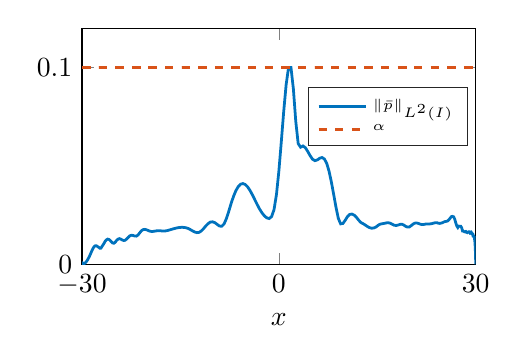
\begin{tikzpicture}

\begin{axis}[%
width=5cm,
height=3cm,
at={(0.0in,0.0in)},
scale only axis,
xmin=-30,
xmax=30,
xlabel={$x$},
xtick={-30,0,30},
ymin=0,
ymax=0.12,
ytick={0,0.1},
legend style={legend cell align=left,align=left,draw=white!15!black,at={(0.98,0.75)}}
]
\addplot [color=mycolor1,solid,line width=1.0pt]
  table[row sep=crcr]{%
-30	0\\
-29.9977410551743	3.57023236110387e-06\\
-29.9909645608861	8.53310014305064e-06\\
-29.9796715376505	1.19702682086754e-05\\
-29.9638636861552	1.8589803064724e-05\\
-29.9435433870045	3.48445088908889e-05\\
-29.9187137003607	0.000107935253624324\\
-29.8893783654833	0.000149288928846725\\
-29.8555418001659	9.09724146659399e-05\\
-29.8172091000707	0.000521624938123296\\
-29.7743860379613	0.000386216091885639\\
-29.7270790628334	0.000348505970597579\\
-29.6752952989434	0.000628524504793603\\
-29.6190425447357	0.000609301045146672\\
-29.5583292716682	0.000650485035385252\\
-29.4931646229365	0.000856206957324206\\
-29.4235584120969	0.00114920381597548\\
-29.3495211215888	0.00140629525496499\\
-29.2710639011559	0.00177725796324325\\
-29.1881985661668	0.0021579339150889\\
-29.1009375958363	0.0026657327033769\\
-29.0092941313456	0.00325194237321933\\
-28.9132819738632	0.00381131211066023\\
-28.812915582467	0.00456398776617423\\
-28.7082100719663	0.00535300209178225\\
-28.5991812106258	0.0061888259505476\\
-28.4858454177911	0.00709177966960147\\
-28.3682197614156	0.00787879220736416\\
-28.2463219554906	0.00860261992396619\\
-28.1201703573772	0.00913383245006255\\
-27.9897839650422	0.00947693739602364\\
-27.8551824141965	0.00952550481802475\\
-27.7163859753386	0.00929131346070304\\
-27.5734155507017	0.00895794957346105\\
-27.4262926711059	0.00864926463274264\\
-27.2750394927157	0.00821792840959545\\
-27.1196787937033	0.00827808516421279\\
-26.9602339708186	0.00914124720962115\\
-26.7967290358655	0.009927552537907\\
-26.6291886120856	0.0108576830743848\\
-26.4576379304506	0.0118672957259352\\
-26.2821028258622	0.0125128748917272\\
-26.1026097332613	0.0128619654959746\\
-25.9191856836476	0.0127274893741163\\
-25.7318583000082	0.0122735347339838\\
-25.540655793158	0.0115300495050292\\
-25.3456069574912	0.0108979851717196\\
-25.1467411666451	0.0107741410517776\\
-24.9440883690764	0.0112663560019861\\
-24.7376790835508	0.0122199117060233\\
-24.5275443945475	0.0128400843042134\\
-24.3137159475778	0.0131104894430098\\
-24.0962259444193	0.0128690897910922\\
-23.8751071382665	0.0124449979058948\\
-23.6503928287982	0.0121705461657551\\
-23.4221168571628	0.0122844339303218\\
-23.1903136008821	0.0129717250019543\\
-22.9550179686738	0.0137698495246454\\
-22.7162653951945	0.0145371813362125\\
-22.4740918357038	0.0148225652624619\\
-22.2285337606488	0.0147386812366384\\
-21.9796281501724	0.0144301046517501\\
-21.727412488544	0.0143914430543338\\
-21.4719247585146	0.0149210488720557\\
-21.2132034355964	0.016042527481337\\
-20.9512874822692	0.0171037142359086\\
-20.686216342112	0.0176915831871546\\
-20.4180299338636	0.0178287447640081\\
-20.1467686454106	0.0175745135960961\\
-19.8724733277052	0.0171757077888302\\
-19.5951852886133	0.0168429375178425\\
-19.3149462866937	0.0167190895620056\\
-19.0317985249094	0.0168497285558084\\
-18.7457846442716	0.0170283399170796\\
-18.4569477174188	0.017134429132711\\
-18.1653312421298	0.0171440335303751\\
-17.870979134773	0.0170365353678009\\
-17.5739357236932	0.0169698234865435\\
-17.2742457425354	0.0170478784028716\\
-16.9719543235084	0.017233499902557\\
-16.6671069905881	0.0175316099832722\\
-16.3597496526614	0.0178240512118858\\
-16.0499285966129	0.0181230500362344\\
-15.7376904803541	0.0184057624214201\\
-15.4230823257966	0.0186448628354295\\
-15.1061515117715	0.0187983294537125\\
-14.7869457668935	0.0188673898234654\\
-14.4655131623737	0.0188148410702877\\
-14.1419021047799	0.0186454032118121\\
-13.8161613287472	0.0182585897469566\\
-13.4883398896382	0.0176971401352366\\
-13.1584871561558	0.0170494211235204\\
-12.8266528029085	0.0164755912582321\\
-12.4928868029291	0.0161588220320923\\
-12.1572394201497	0.0163026589658519\\
-11.8197612018314	0.0170528838353961\\
-11.4805029709527	0.0181761961297825\\
-11.1395158185551	0.0195678640403457\\
-10.7968510960496	0.0207192561215126\\
-10.452560407483	0.0215162239956649\\
-10.1066956017666	0.0216639484387164\\
-9.75930876486789	0.0212411710231197\\
-9.41045221196674	0.0203772521506555\\
-9.06017847957684	0.0195207897245672\\
-8.70854031763387	0.0193858497884021\\
-8.35559068155159	0.0205860492673538\\
-8.00138272424695	0.0232688151220888\\
-7.64596978813544	0.0269068176197282\\
-7.28940539709792	0.0308633519957826\\
-6.93174324842013	0.0344344852721056\\
-6.57303720470609	0.0373440203471834\\
-6.21334128576655	0.0394577842081594\\
-5.85270966048385	0.0407290314085478\\
-5.49119663865423	0.0410925923089755\\
-5.12885666280904	0.0406186779702271\\
-4.76574430001584	0.0394019924569551\\
-4.40191423366085	0.0375970157633319\\
-4.03742125521378	0.0353598580766045\\
-3.67232025597648	0.0329038346196463\\
-3.30666621881649	0.0304355829997441\\
-2.94051420988682	0.028149985864292\\
-2.57391937033319	0.0262038839318964\\
-2.20693690799002	0.0246758319200349\\
-1.83962208906626	0.0236489817241336\\
-1.47203022982254	0.0233238684624988\\
-1.10421668824077	0.024304030347741\\
-0.736236855687364	0.027917800034882\\
-0.368146148571595	0.0355778169850728\\
1.83697019872103e-15	0.0474954835006233\\
0.368146148571598	0.0623406562409012\\
0.736236855687368	0.0777604923487494\\
1.10421668824077	0.0912926232999088\\
1.47203022982254	0.100085679627589\\
1.83962208906626	0.100083599331388\\
2.20693690799002	0.0892258460707249\\
2.5739193703332	0.0726505975545132\\
2.94051420988682	0.0613931358398691\\
3.3066662188165	0.0595567126046281\\
3.67232025597649	0.0602041910706215\\
4.03742125521379	0.0592872626782237\\
4.40191423366085	0.0574009141457593\\
4.76574430001584	0.0552229677646754\\
5.12885666280904	0.0534566043806536\\
5.49119663865423	0.0527292858548513\\
5.85270966048385	0.0530914042228684\\
6.21334128576656	0.0539247485279318\\
6.57303720470609	0.0543340387587823\\
6.93174324842014	0.0535806510196285\\
7.28940539709792	0.0513597039018075\\
7.64596978813544	0.0473469454534553\\
8.00138272424695	0.0418415471147308\\
8.35559068155159	0.0354547743572128\\
8.70854031763387	0.0289476767661415\\
9.06017847957685	0.0233787032833489\\
9.41045221196675	0.0206072309815088\\
9.75930876486789	0.0208268717443634\\
10.1066956017666	0.0224460247686763\\
10.452560407483	0.0243198225649514\\
10.7968510960496	0.0254073370787006\\
11.1395158185551	0.0256056701091524\\
11.4805029709527	0.0250405495965697\\
11.8197612018314	0.0239028882901328\\
12.1572394201497	0.0224988646875092\\
12.4928868029291	0.0213078783524966\\
12.8266528029085	0.0207233759093186\\
13.1584871561558	0.0200427434575663\\
13.4883398896382	0.0192714083319551\\
13.8161613287472	0.0187013045192922\\
14.1419021047799	0.0183955024659071\\
14.4655131623737	0.0185453758443638\\
14.7869457668935	0.0190025592583767\\
15.1061515117715	0.0198452053645\\
15.4230823257966	0.020474646739096\\
15.7376904803541	0.020671943184728\\
16.0499285966129	0.0208549969354354\\
16.3597496526614	0.0211016992109799\\
16.6671069905881	0.0212000232884192\\
16.9719543235084	0.0209541738592988\\
17.2742457425354	0.0204331885552769\\
17.5739357236932	0.0199179225436769\\
17.870979134773	0.0197904500651445\\
18.1653312421298	0.0200191049842221\\
18.4569477174188	0.0203527832372959\\
18.7457846442716	0.020423213824348\\
19.0317985249094	0.0200288316039912\\
19.3149462866937	0.0193767425308158\\
19.5951852886133	0.018977682059864\\
19.8724733277052	0.0190318813098892\\
20.1467686454106	0.0196721278373523\\
20.4180299338636	0.0204257435784195\\
20.686216342112	0.0209505426697072\\
20.9512874822692	0.0210918867362902\\
21.2132034355964	0.0208906291460385\\
21.4719247585146	0.0205586368517346\\
21.727412488544	0.0203017977101973\\
21.9796281501724	0.0202431019527747\\
22.2285337606488	0.0204435080434696\\
22.4740918357038	0.0205517646511076\\
22.7162653951945	0.0205665525832828\\
22.9550179686738	0.0205865794603954\\
23.1903136008821	0.0206542377603775\\
23.4221168571628	0.0208487787281602\\
23.6503928287982	0.0210622495882637\\
23.8751071382665	0.0212238248073837\\
24.0962259444193	0.0212130695057624\\
24.3137159475778	0.0209252264384814\\
24.5275443945475	0.0208515253926663\\
24.7376790835508	0.0210159863838729\\
24.9440883690764	0.0212213065545162\\
25.1467411666451	0.0215721122144463\\
25.3456069574912	0.0217915459419925\\
25.540655793158	0.0219007604561026\\
25.7318583000082	0.0221366917140012\\
25.9191856836476	0.0227426346903602\\
26.1026097332613	0.0235212844977578\\
26.2821028258622	0.0242942719970661\\
26.4576379304507	0.024427029026494\\
26.6291886120856	0.0242150845539571\\
26.7967290358655	0.0230238749964381\\
26.9602339708186	0.0211043255390472\\
27.1196787937033	0.0194917202895318\\
27.2750394927157	0.0187267554693191\\
27.4262926711059	0.0194845494810254\\
27.5734155507017	0.0194109168987053\\
27.7163859753386	0.0194145114552722\\
27.8551824141965	0.0186563743626293\\
27.9897839650422	0.0169626709813463\\
28.1201703573772	0.0169407739667706\\
28.2463219554906	0.016614288033099\\
28.3682197614156	0.0165346879189745\\
28.4858454177911	0.0167406249286063\\
28.5991812106258	0.0163027103136246\\
28.7082100719663	0.016130558099788\\
28.812915582467	0.0163230990259903\\
28.9132819738632	0.0166576198619076\\
29.0092941313456	0.0166488898285122\\
29.1009375958363	0.0161484230782587\\
29.1881985661668	0.016469319238394\\
29.2710639011559	0.0165214366820829\\
29.3495211215888	0.0158354267531479\\
29.4235584120969	0.0159050181891397\\
29.4931646229365	0.015596447473943\\
29.5583292716682	0.0147732966579492\\
29.6190425447358	0.0148864940147152\\
29.6752952989434	0.0143932671620171\\
29.7270790628334	0.0139975072676901\\
29.7743860379613	0.0139547677621965\\
29.8172091000707	0.0127615278154232\\
29.8555418001659	0.0120978050532036\\
29.8893783654833	0.0105592893647438\\
29.9187137003607	0.00893513662775621\\
29.9435433870045	0.00692423165331794\\
29.9638636861552	0.00482909604805362\\
29.9796715376505	0.00294932702092065\\
29.9909645608861	0.00139792700304437\\
29.9977410551743	0.000463194155612154\\
30	1.29872537992108e-17\\
};
\addlegendentry{\tiny$\|\bar p\|_{L^2(I)}$};

\addplot [color=mycolor2,dashed,line width=1.0pt]
  table[row sep=crcr]{%
-30	0.1\\
-29.9977410551743	0.1\\
-29.9909645608861	0.1\\
-29.9796715376505	0.1\\
-29.9638636861552	0.1\\
-29.9435433870045	0.1\\
-29.9187137003607	0.1\\
-29.8893783654833	0.1\\
-29.8555418001659	0.1\\
-29.8172091000707	0.1\\
-29.7743860379613	0.1\\
-29.7270790628334	0.1\\
-29.6752952989434	0.1\\
-29.6190425447357	0.1\\
-29.5583292716682	0.1\\
-29.4931646229365	0.1\\
-29.4235584120969	0.1\\
-29.3495211215888	0.1\\
-29.2710639011559	0.1\\
-29.1881985661668	0.1\\
-29.1009375958363	0.1\\
-29.0092941313456	0.1\\
-28.9132819738632	0.1\\
-28.812915582467	0.1\\
-28.7082100719663	0.1\\
-28.5991812106258	0.1\\
-28.4858454177911	0.1\\
-28.3682197614156	0.1\\
-28.2463219554906	0.1\\
-28.1201703573772	0.1\\
-27.9897839650422	0.1\\
-27.8551824141965	0.1\\
-27.7163859753386	0.1\\
-27.5734155507017	0.1\\
-27.4262926711059	0.1\\
-27.2750394927157	0.1\\
-27.1196787937033	0.1\\
-26.9602339708186	0.1\\
-26.7967290358655	0.1\\
-26.6291886120856	0.1\\
-26.4576379304506	0.1\\
-26.2821028258622	0.1\\
-26.1026097332613	0.1\\
-25.9191856836476	0.1\\
-25.7318583000082	0.1\\
-25.540655793158	0.1\\
-25.3456069574912	0.1\\
-25.1467411666451	0.1\\
-24.9440883690764	0.1\\
-24.7376790835508	0.1\\
-24.5275443945475	0.1\\
-24.3137159475778	0.1\\
-24.0962259444193	0.1\\
-23.8751071382665	0.1\\
-23.6503928287982	0.1\\
-23.4221168571628	0.1\\
-23.1903136008821	0.1\\
-22.9550179686738	0.1\\
-22.7162653951945	0.1\\
-22.4740918357038	0.1\\
-22.2285337606488	0.1\\
-21.9796281501724	0.1\\
-21.727412488544	0.1\\
-21.4719247585146	0.1\\
-21.2132034355964	0.1\\
-20.9512874822692	0.1\\
-20.686216342112	0.1\\
-20.4180299338636	0.1\\
-20.1467686454106	0.1\\
-19.8724733277052	0.1\\
-19.5951852886133	0.1\\
-19.3149462866937	0.1\\
-19.0317985249094	0.1\\
-18.7457846442716	0.1\\
-18.4569477174188	0.1\\
-18.1653312421298	0.1\\
-17.870979134773	0.1\\
-17.5739357236932	0.1\\
-17.2742457425354	0.1\\
-16.9719543235084	0.1\\
-16.6671069905881	0.1\\
-16.3597496526614	0.1\\
-16.0499285966129	0.1\\
-15.7376904803541	0.1\\
-15.4230823257966	0.1\\
-15.1061515117715	0.1\\
-14.7869457668935	0.1\\
-14.4655131623737	0.1\\
-14.1419021047799	0.1\\
-13.8161613287472	0.1\\
-13.4883398896382	0.1\\
-13.1584871561558	0.1\\
-12.8266528029085	0.1\\
-12.4928868029291	0.1\\
-12.1572394201497	0.1\\
-11.8197612018314	0.1\\
-11.4805029709527	0.1\\
-11.1395158185551	0.1\\
-10.7968510960496	0.1\\
-10.452560407483	0.1\\
-10.1066956017666	0.1\\
-9.75930876486789	0.1\\
-9.41045221196674	0.1\\
-9.06017847957684	0.1\\
-8.70854031763387	0.1\\
-8.35559068155159	0.1\\
-8.00138272424695	0.1\\
-7.64596978813544	0.1\\
-7.28940539709792	0.1\\
-6.93174324842013	0.1\\
-6.57303720470609	0.1\\
-6.21334128576655	0.1\\
-5.85270966048385	0.1\\
-5.49119663865423	0.1\\
-5.12885666280904	0.1\\
-4.76574430001584	0.1\\
-4.40191423366085	0.1\\
-4.03742125521378	0.1\\
-3.67232025597648	0.1\\
-3.30666621881649	0.1\\
-2.94051420988682	0.1\\
-2.57391937033319	0.1\\
-2.20693690799002	0.1\\
-1.83962208906626	0.1\\
-1.47203022982254	0.1\\
-1.10421668824077	0.1\\
-0.736236855687364	0.1\\
-0.368146148571595	0.1\\
1.83697019872103e-15	0.1\\
0.368146148571598	0.1\\
0.736236855687368	0.1\\
1.10421668824077	0.1\\
1.47203022982254	0.1\\
1.83962208906626	0.1\\
2.20693690799002	0.1\\
2.5739193703332	0.1\\
2.94051420988682	0.1\\
3.3066662188165	0.1\\
3.67232025597649	0.1\\
4.03742125521379	0.1\\
4.40191423366085	0.1\\
4.76574430001584	0.1\\
5.12885666280904	0.1\\
5.49119663865423	0.1\\
5.85270966048385	0.1\\
6.21334128576656	0.1\\
6.57303720470609	0.1\\
6.93174324842014	0.1\\
7.28940539709792	0.1\\
7.64596978813544	0.1\\
8.00138272424695	0.1\\
8.35559068155159	0.1\\
8.70854031763387	0.1\\
9.06017847957685	0.1\\
9.41045221196675	0.1\\
9.75930876486789	0.1\\
10.1066956017666	0.1\\
10.452560407483	0.1\\
10.7968510960496	0.1\\
11.1395158185551	0.1\\
11.4805029709527	0.1\\
11.8197612018314	0.1\\
12.1572394201497	0.1\\
12.4928868029291	0.1\\
12.8266528029085	0.1\\
13.1584871561558	0.1\\
13.4883398896382	0.1\\
13.8161613287472	0.1\\
14.1419021047799	0.1\\
14.4655131623737	0.1\\
14.7869457668935	0.1\\
15.1061515117715	0.1\\
15.4230823257966	0.1\\
15.7376904803541	0.1\\
16.0499285966129	0.1\\
16.3597496526614	0.1\\
16.6671069905881	0.1\\
16.9719543235084	0.1\\
17.2742457425354	0.1\\
17.5739357236932	0.1\\
17.870979134773	0.1\\
18.1653312421298	0.1\\
18.4569477174188	0.1\\
18.7457846442716	0.1\\
19.0317985249094	0.1\\
19.3149462866937	0.1\\
19.5951852886133	0.1\\
19.8724733277052	0.1\\
20.1467686454106	0.1\\
20.4180299338636	0.1\\
20.686216342112	0.1\\
20.9512874822692	0.1\\
21.2132034355964	0.1\\
21.4719247585146	0.1\\
21.727412488544	0.1\\
21.9796281501724	0.1\\
22.2285337606488	0.1\\
22.4740918357038	0.1\\
22.7162653951945	0.1\\
22.9550179686738	0.1\\
23.1903136008821	0.1\\
23.4221168571628	0.1\\
23.6503928287982	0.1\\
23.8751071382665	0.1\\
24.0962259444193	0.1\\
24.3137159475778	0.1\\
24.5275443945475	0.1\\
24.7376790835508	0.1\\
24.9440883690764	0.1\\
25.1467411666451	0.1\\
25.3456069574912	0.1\\
25.540655793158	0.1\\
25.7318583000082	0.1\\
25.9191856836476	0.1\\
26.1026097332613	0.1\\
26.2821028258622	0.1\\
26.4576379304507	0.1\\
26.6291886120856	0.1\\
26.7967290358655	0.1\\
26.9602339708186	0.1\\
27.1196787937033	0.1\\
27.2750394927157	0.1\\
27.4262926711059	0.1\\
27.5734155507017	0.1\\
27.7163859753386	0.1\\
27.8551824141965	0.1\\
27.9897839650422	0.1\\
28.1201703573772	0.1\\
28.2463219554906	0.1\\
28.3682197614156	0.1\\
28.4858454177911	0.1\\
28.5991812106258	0.1\\
28.7082100719663	0.1\\
28.812915582467	0.1\\
28.9132819738632	0.1\\
29.0092941313456	0.1\\
29.1009375958363	0.1\\
29.1881985661668	0.1\\
29.2710639011559	0.1\\
29.3495211215888	0.1\\
29.4235584120969	0.1\\
29.4931646229365	0.1\\
29.5583292716682	0.1\\
29.6190425447358	0.1\\
29.6752952989434	0.1\\
29.7270790628334	0.1\\
29.7743860379613	0.1\\
29.8172091000707	0.1\\
29.8555418001659	0.1\\
29.8893783654833	0.1\\
29.9187137003607	0.1\\
29.9435433870045	0.1\\
29.9638636861552	0.1\\
29.9796715376505	0.1\\
29.9909645608861	0.1\\
29.9977410551743	0.1\\
30	0.1\\
};
\addlegendentry{\tiny $\alpha$};

\end{axis}
\end{tikzpicture}%}
\subfloat{% This file was created by matlab2tikz.
% Minimal pgfplots version: 1.3
%
%The latest updates can be retrieved from
%  http://www.mathworks.com/matlabcentral/fileexchange/22022-matlab2tikz
%where you can also make suggestions and rate matlab2tikz.
%
\definecolor{mycolor1}{rgb}{0.00000,0.44700,0.74100}%
%
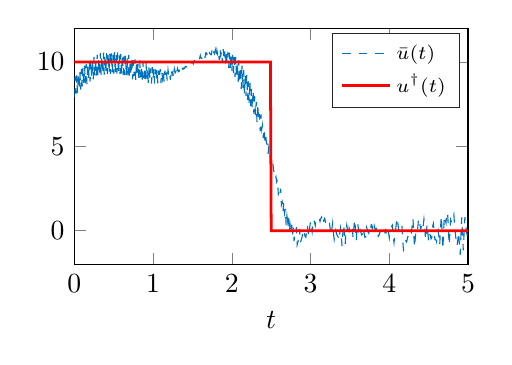
\begin{tikzpicture}

\begin{axis}[%
width=5cm,
height=3cm,
at={(0.0in,0.0in)},
scale only axis,
xmin=0,
xmax=5,
xlabel={$t$},
ymin=-2,
ymax=12,
legend style={legend cell align=left,align=left,draw=white!15!black}
]
\addplot [color=mycolor1,dashed]
  table[row sep=crcr]{%
0	7.91291543263887\\
0.01	9.1598361587429\\
0.02	8.11826905373297\\
0.03	9.20039127330638\\
0.04	8.15620502557183\\
0.05	9.39319056419603\\
0.06	8.34879417745493\\
0.07	9.4663228111888\\
0.08	8.36029942685653\\
0.09	9.59516535470859\\
0.1	8.55339434088673\\
0.11	9.7000314524602\\
0.12	8.53664304517838\\
0.13	9.78016671752941\\
0.14	8.73516611789048\\
0.15	9.89095285175104\\
0.16	8.69462891739611\\
0.17	9.9605778138011\\
0.18	8.88948541379508\\
0.19	10.0373496847621\\
0.2	8.83730966696748\\
0.21	10.1383321039629\\
0.22	9.01183104348255\\
0.23	10.1423112517368\\
0.24	8.96840240122722\\
0.25	10.3009699039133\\
0.26	9.10386874567987\\
0.27	10.2204193099131\\
0.28	9.08798576162821\\
0.29	10.4337231620634\\
0.3	9.16955234652158\\
0.31	10.2937428418141\\
0.32	9.1892697377079\\
0.33	10.5204089382484\\
0.34	9.21442770341053\\
0.35	10.3750785302683\\
0.36	9.2647304372216\\
0.37	10.5502459463597\\
0.38	9.24808906916802\\
0.39	10.4649319094994\\
0.4	9.31164375380587\\
0.41	10.5304462857288\\
0.42	9.27766032610328\\
0.43	10.5520712867498\\
0.44	9.32888393504225\\
0.45	10.4840545716626\\
0.46	9.3011688611746\\
0.47	10.6137768657796\\
0.48	9.31937225830536\\
0.49	10.4386985612375\\
0.5	9.31294892941539\\
0.51	10.6252896111959\\
0.52	9.29393398310033\\
0.53	10.4159273551536\\
0.54	9.30705126562081\\
0.55	10.5741855539586\\
0.56	9.26465038708096\\
0.57	10.4222014266454\\
0.58	9.27680729278988\\
0.59	10.468735732007\\
0.6	9.23902116215973\\
0.61	10.4439082066316\\
0.62	9.21990422409179\\
0.63	10.3357771426825\\
0.64	9.22041563467732\\
0.65	10.4515629663194\\
0.66	9.14196291644459\\
0.67	10.210721925444\\
0.68	9.20723357136437\\
0.69	10.4138230663213\\
0.7	9.05303129619069\\
0.71	10.1237383291519\\
0.72	9.19276581708126\\
0.73	10.3136357744226\\
0.74	8.96389423021389\\
0.75	10.0863025095857\\
0.76	9.1700424125963\\
0.77	10.1574266643172\\
0.78	8.88457618207509\\
0.79	10.0848793199984\\
0.8	9.13640623156797\\
0.81	9.97386047464332\\
0.82	8.82170880779454\\
0.83	10.0871427559051\\
0.84	9.0937112533388\\
0.85	9.80322102803655\\
0.86	8.77648479270053\\
0.87	10.0581400209329\\
0.88	9.047051056254\\
0.89	9.68072448856636\\
0.9	8.74638900939656\\
0.91	9.97734778871054\\
0.92	9.00389658252982\\
0.93	9.62073960757594\\
0.94	8.72843186448482\\
0.95	9.84843364639272\\
0.96	8.97218204820567\\
0.97	9.61095905594855\\
0.98	8.72047241993349\\
0.99	9.69819478974472\\
1	8.95778375474229\\
1.01	9.62027437212401\\
1.02	8.7213400003744\\
1.03	9.56488212656327\\
1.04	8.96386337185315\\
1.05	9.61545220660623\\
1.06	8.73151689351057\\
1.07	9.48039265107201\\
1.08	8.9918703255748\\
1.09	9.5773653796552\\
1.1	8.75367829304137\\
1.11	9.45576180209278\\
1.12	9.0415362801187\\
1.13	9.50946594035284\\
1.14	8.79203174932956\\
1.15	9.47853926836183\\
1.16	9.10945703206162\\
1.17	9.43509107856447\\
1.18	8.85144428330307\\
1.19	9.52259891479034\\
1.2	9.18884113199928\\
1.21	9.38475025018099\\
1.22	8.93723209758236\\
1.23	9.56305340964336\\
1.24	9.27190850059\\
1.25	9.38033538325325\\
1.26	9.0541067554355\\
1.27	9.58768542155303\\
1.28	9.35340700657202\\
1.29	9.42606977280593\\
1.3	9.20279247927414\\
1.31	9.60005547140211\\
1.32	9.43316110605361\\
1.33	9.5110931757958\\
1.34	9.3761958494525\\
1.35	9.61406569826775\\
1.36	9.51691307142266\\
1.37	9.61938319545012\\
1.38	9.55899595787526\\
1.39	9.64419597279456\\
1.4	9.61498121734047\\
1.41	9.73819385651491\\
1.42	9.73209914739428\\
1.43	9.69848021367454\\
1.44	9.7379131829315\\
1.45	9.85967845470171\\
1.46	9.87951429244614\\
1.47	9.77894206599219\\
1.48	9.88989312688006\\
1.49	9.9771706849894\\
1.5	9.99392295143071\\
1.51	9.88694619024977\\
1.52	10.0633999634502\\
1.53	10.0818691864907\\
1.54	10.0786287264965\\
1.55	10.0256004723257\\
1.56	10.2389085759419\\
1.57	10.164970172985\\
1.58	10.1453997069058\\
1.59	10.1941921809213\\
1.6	10.3902240211633\\
1.61	10.2252503291667\\
1.62	10.20897499919\\
1.63	10.3786812138803\\
1.64	10.4924745165288\\
1.65	10.2757628058538\\
1.66	10.2800662366752\\
1.67	10.5487154624061\\
1.68	10.5291007444751\\
1.69	10.3408827084187\\
1.7	10.359364466034\\
1.71	10.6684412655115\\
1.72	10.4959759797973\\
1.73	10.4407093574391\\
1.74	10.4346699650219\\
1.75	10.7170495605203\\
1.76	10.4023212275576\\
1.77	10.571542535727\\
1.78	10.4822442211312\\
1.79	10.7043545797907\\
1.8	10.2680204357777\\
1.81	10.6988211905807\\
1.82	10.4728729637077\\
1.83	10.6663326740261\\
1.84	10.1165588083999\\
1.85	10.7731094640472\\
1.86	10.382285796337\\
1.87	10.6387883793914\\
1.88	9.96415686849502\\
1.89	10.7619044609435\\
1.9	10.2029505171302\\
1.91	10.6264171170682\\
1.92	9.80942807897377\\
1.93	10.6735403637934\\
1.94	9.95071644656231\\
1.95	10.5933772830862\\
1.96	9.63141398869835\\
1.97	10.5500321965774\\
1.98	9.65919153587638\\
1.99	10.488523343145\\
2	9.4017868919986\\
2.01	10.4283214259181\\
2.02	9.36075697385625\\
2.03	10.2895392702569\\
2.04	9.10699057351527\\
2.05	10.2994464746537\\
2.06	9.06461999959823\\
2.07	10.0279831445426\\
2.08	8.76423248583393\\
2.09	10.1051689385698\\
2.1	8.75040750602501\\
2.11	9.76540715367903\\
2.12	8.4135368364006\\
2.13	9.7849641787188\\
2.14	8.38871615323693\\
2.15	9.53161906361366\\
2.16	8.08432885125272\\
2.17	9.33843030012972\\
2.18	7.97671860058118\\
2.19	9.27887444649619\\
2.2	7.76172419863197\\
2.21	8.841526002355\\
2.22	7.55529048894905\\
2.23	8.90528640523079\\
2.24	7.38976813553054\\
2.25	8.38547456383091\\
2.26	7.17965628277852\\
2.27	8.34285195955299\\
2.28	6.92330857986079\\
2.29	7.98216975132392\\
2.3	6.85629728748043\\
2.31	7.63404306170337\\
2.32	6.38846053561076\\
2.33	7.53040142771451\\
2.34	6.50582095521609\\
2.35	6.91050839319077\\
2.36	5.88349106271568\\
2.37	6.89671627993435\\
2.38	6.00960059327186\\
2.39	6.27221786715344\\
2.4	5.49218639433263\\
2.41	6.05130281570879\\
2.42	5.32331748130282\\
2.43	5.67903611405404\\
2.44	5.17525860505503\\
2.45	5.12105425991355\\
2.46	4.55246230102491\\
2.47	4.98081534817956\\
2.48	4.76213201402197\\
2.49	4.28184134337524\\
2.5	3.88698418115061\\
2.51	4.0807271647756\\
2.52	4.09332984087973\\
2.53	3.58252938298995\\
2.54	3.42101047737663\\
2.55	3.06983374468946\\
2.56	3.1988143928048\\
2.57	2.89442830505235\\
2.58	3.03353094113127\\
2.59	2.170170194976\\
2.6	2.31584730309524\\
2.61	2.06570825830988\\
2.62	2.49106619948171\\
2.63	1.52109776408433\\
2.64	1.68245761943255\\
2.65	1.12812780013334\\
2.66	1.70684752342356\\
2.67	1.03969877149975\\
2.68	1.29599598413911\\
2.69	0.315895989536414\\
2.7	0.882077494159358\\
2.71	0.527577079088768\\
2.72	0.916618554541077\\
2.73	-0.150817671469746\\
2.74	0.337755399857441\\
2.75	-0.0812434454628767\\
2.76	0.35124068323254\\
2.77	-0.283811211070473\\
2.78	0.185200854209048\\
2.79	-0.615537263647049\\
2.8	-0.28732194065447\\
2.81	-0.294755328495483\\
2.82	0.206372231642445\\
2.83	-0.838799040133334\\
2.84	-0.661540395366378\\
2.85	-0.352611440888413\\
2.86	0.102408273751962\\
2.87	-0.699987604173825\\
2.88	-0.563255587136724\\
2.89	-0.41732081857037\\
2.9	-0.173268946832859\\
2.91	-0.369649330340295\\
2.92	-0.133407067704229\\
2.93	-0.339461024435411\\
2.94	-0.391393607767876\\
2.95	-0.0430591741171409\\
2.96	0.304420450192123\\
2.97	-0.0793022705343688\\
2.98	-0.340474639589047\\
2.99	0.227864880871886\\
3	0.562575698684552\\
3.01	0.242101726342762\\
3.02	-0.0500013652321047\\
3.03	0.478537252776064\\
3.04	0.664843382384704\\
3.05	0.49487360506756\\
3.06	0.308983447487042\\
3.07	0.678255404666969\\
3.08	0.664879770832304\\
3.09	0.654828218785742\\
3.1	0.62179138783255\\
3.11	0.734488569055431\\
3.12	0.555336274842819\\
3.13	0.728977195373969\\
3.14	0.813351473825182\\
3.15	0.637527036614403\\
3.16	0.398707567056773\\
3.17	0.657289610254261\\
3.18	0.735638789697709\\
3.19	0.483380300464341\\
3.2	0.361802262214387\\
3.21	0.399169199373583\\
3.22	0.298137244383118\\
3.23	0.318104216534974\\
3.24	0.464895279194322\\
3.25	0.0738195066042605\\
3.26	-0.269417683104299\\
3.27	0.0868140018023865\\
3.28	0.434007778447394\\
3.29	-0.131674044986584\\
3.3	-0.521769540451258\\
3.31	-0.196504544957488\\
3.32	0.0292044335470101\\
3.33	-0.188729734316013\\
3.34	-0.285276616926706\\
3.35	-0.36699750352477\\
3.36	-0.565699920445867\\
3.37	-0.194216069190981\\
3.38	0.144792484363308\\
3.39	-0.31491239856844\\
3.4	-0.911360660608855\\
3.41	-0.153092935410974\\
3.42	0.392964339215029\\
3.43	-0.148594974685983\\
3.44	-0.789491321619763\\
3.45	-0.00754960217829962\\
3.46	0.332991324327846\\
3.47	-0.00323643756944936\\
3.48	-0.299188055230321\\
3.49	0.162169524814356\\
3.5	-0.0038424716978847\\
3.51	0.116039488730228\\
3.52	0.321067115259539\\
3.53	0.207970755336865\\
3.54	-0.440945370289821\\
3.55	0.170404254318046\\
3.56	0.66783861773903\\
3.57	0.140467588487148\\
3.58	-0.587719700742719\\
3.59	0.0882960142627171\\
3.6	0.39931957989513\\
3.61	0.00665299128648148\\
3.62	-0.330287598026222\\
3.63	0.030630993365495\\
3.64	-0.114089609022113\\
3.65	-0.243869749556597\\
3.66	-0.192838057649527\\
3.67	0.165293437332553\\
3.68	-0.14345678698667\\
3.69	-0.392178848626113\\
3.7	-0.364353914290983\\
3.71	0.212626042178715\\
3.72	0.0780657034436202\\
3.73	-0.0637139868728213\\
3.74	-0.155808858511257\\
3.75	0.00982793388190498\\
3.76	-0.093445174919224\\
3.77	0.356283542076378\\
3.78	0.327106205524709\\
3.79	-0.00617590105242038\\
3.8	-0.11659621414569\\
3.81	0.266506711582709\\
3.82	0.0718296684521708\\
3.83	0.0504808260584053\\
3.84	0.21246721596866\\
3.85	0.0920554352169678\\
3.86	-0.331763902626949\\
3.87	-0.25952129224006\\
3.88	-0.0920615932512136\\
3.89	-0.0274207663873606\\
3.9	-0.193894433871259\\
3.91	-0.198769874432666\\
3.92	-0.300921676003001\\
3.93	-0.305520980279453\\
3.94	-0.266164125207672\\
3.95	0.0288296862483088\\
3.96	-0.0963120905873494\\
3.97	0.0613485079792879\\
3.98	0.226826218397348\\
3.99	-0.0946539322495629\\
4	-0.423236363105417\\
4.01	-0.0318032991607105\\
4.02	0.143397779312374\\
4.03	0.257118430094821\\
4.04	0.3329781590733\\
4.05	-0.326541090908595\\
4.06	-0.707822416389054\\
4.07	-0.227596003637102\\
4.08	0.045586256950527\\
4.09	0.459296843672624\\
4.1	0.764854765333776\\
4.11	0.377288317616756\\
4.12	0.0517157215914118\\
4.13	0.15434297559729\\
4.14	0.294702155677369\\
4.15	0.236325850956347\\
4.16	0.358825202076824\\
4.17	-0.515698961067057\\
4.18	-1.1451330391139\\
4.19	-1.0308265661549\\
4.2	-0.635287020056475\\
4.21	-0.600817084159598\\
4.22	-0.668669328503694\\
4.23	-0.448078543499011\\
4.24	-0.289038709571604\\
4.25	-0.341279512361389\\
4.26	-0.286059218789013\\
4.27	0.00626311501234024\\
4.28	-0.0933526980702727\\
4.29	0.279319074842659\\
4.3	0.736540757557926\\
4.31	-0.0542884816856619\\
4.32	-0.981900496231251\\
4.33	-0.434870358839679\\
4.34	0.017217790244553\\
4.35	0.177942604943235\\
4.36	0.0816928102436293\\
4.37	0.651516894487539\\
4.38	0.740898031138643\\
4.39	0.325440301049218\\
4.4	0.0944105556023418\\
4.41	0.319393631107104\\
4.42	0.0847853426675438\\
4.43	0.290620870877548\\
4.44	0.68790153179231\\
4.45	0.259346338705535\\
4.46	-0.52315975915686\\
4.47	-0.130827821776045\\
4.48	0.358475533768608\\
4.49	-0.177690950277121\\
4.5	-0.657449040917248\\
4.51	-0.250389544786929\\
4.52	-0.253669078522667\\
4.53	-0.483256528082345\\
4.54	-0.398660224424987\\
4.55	0.2623644033224\\
4.56	0.42367320039832\\
4.57	-0.103084749369844\\
4.58	-0.521654722409814\\
4.59	-0.511689557964126\\
4.6	-0.658084224758072\\
4.61	-0.250414550515474\\
4.62	-0.00324948302434027\\
4.63	-0.349539378514784\\
4.64	-0.844773872116351\\
4.65	0.0344883205933965\\
4.66	0.887981490500239\\
4.67	0.0244014788908499\\
4.68	-1.10694753862385\\
4.69	-0.00225527863815959\\
4.7	0.881906683665367\\
4.71	0.678672822700904\\
4.72	0.468207299039329\\
4.73	1.02977329691219\\
4.74	1.09147802372861\\
4.75	0.187087516066517\\
4.76	-0.853800671677569\\
4.77	-0.0806594175746827\\
4.78	0.652814469929822\\
4.79	0.509149344790684\\
4.8	0.535797318428041\\
4.81	0.804567350428566\\
4.82	0.964357120052231\\
4.83	0.253294384315545\\
4.84	-0.202000143655378\\
4.85	-0.619754119827078\\
4.86	-0.915038306402655\\
4.87	-0.540518784557565\\
4.88	-0.094786690387665\\
4.89	-0.774434916453677\\
4.9	-1.43214054599743\\
4.91	-0.247530354773515\\
4.92	0.794758855440092\\
4.93	-0.197374209904392\\
4.94	-1.15988995141328\\
4.95	-0.137119165978102\\
4.96	0.802642483099741\\
4.97	0.3499942470816\\
4.98	-0.0965501523677729\\
4.99	-0.277511759563525\\
5	-0.459073018346663\\
};
\addlegendentry{\scriptsize$\bar u(t)$};

\addplot [color=red,solid,line width=1.0pt]
  table[row sep=crcr]{%
0	10\\
0.01	10\\
0.02	10\\
0.03	10\\
0.04	10\\
0.05	10\\
0.06	10\\
0.07	10\\
0.08	10\\
0.09	10\\
0.1	10\\
0.11	10\\
0.12	10\\
0.13	10\\
0.14	10\\
0.15	10\\
0.16	10\\
0.17	10\\
0.18	10\\
0.19	10\\
0.2	10\\
0.21	10\\
0.22	10\\
0.23	10\\
0.24	10\\
0.25	10\\
0.26	10\\
0.27	10\\
0.28	10\\
0.29	10\\
0.3	10\\
0.31	10\\
0.32	10\\
0.33	10\\
0.34	10\\
0.35	10\\
0.36	10\\
0.37	10\\
0.38	10\\
0.39	10\\
0.4	10\\
0.41	10\\
0.42	10\\
0.43	10\\
0.44	10\\
0.45	10\\
0.46	10\\
0.47	10\\
0.48	10\\
0.49	10\\
0.5	10\\
0.51	10\\
0.52	10\\
0.53	10\\
0.54	10\\
0.55	10\\
0.56	10\\
0.57	10\\
0.58	10\\
0.59	10\\
0.6	10\\
0.61	10\\
0.62	10\\
0.63	10\\
0.64	10\\
0.65	10\\
0.66	10\\
0.67	10\\
0.68	10\\
0.69	10\\
0.7	10\\
0.71	10\\
0.72	10\\
0.73	10\\
0.74	10\\
0.75	10\\
0.76	10\\
0.77	10\\
0.78	10\\
0.79	10\\
0.8	10\\
0.81	10\\
0.82	10\\
0.83	10\\
0.84	10\\
0.85	10\\
0.86	10\\
0.87	10\\
0.88	10\\
0.89	10\\
0.9	10\\
0.91	10\\
0.92	10\\
0.93	10\\
0.94	10\\
0.95	10\\
0.96	10\\
0.97	10\\
0.98	10\\
0.99	10\\
1	10\\
1.01	10\\
1.02	10\\
1.03	10\\
1.04	10\\
1.05	10\\
1.06	10\\
1.07	10\\
1.08	10\\
1.09	10\\
1.1	10\\
1.11	10\\
1.12	10\\
1.13	10\\
1.14	10\\
1.15	10\\
1.16	10\\
1.17	10\\
1.18	10\\
1.19	10\\
1.2	10\\
1.21	10\\
1.22	10\\
1.23	10\\
1.24	10\\
1.25	10\\
1.26	10\\
1.27	10\\
1.28	10\\
1.29	10\\
1.3	10\\
1.31	10\\
1.32	10\\
1.33	10\\
1.34	10\\
1.35	10\\
1.36	10\\
1.37	10\\
1.38	10\\
1.39	10\\
1.4	10\\
1.41	10\\
1.42	10\\
1.43	10\\
1.44	10\\
1.45	10\\
1.46	10\\
1.47	10\\
1.48	10\\
1.49	10\\
1.5	10\\
1.51	10\\
1.52	10\\
1.53	10\\
1.54	10\\
1.55	10\\
1.56	10\\
1.57	10\\
1.58	10\\
1.59	10\\
1.6	10\\
1.61	10\\
1.62	10\\
1.63	10\\
1.64	10\\
1.65	10\\
1.66	10\\
1.67	10\\
1.68	10\\
1.69	10\\
1.7	10\\
1.71	10\\
1.72	10\\
1.73	10\\
1.74	10\\
1.75	10\\
1.76	10\\
1.77	10\\
1.78	10\\
1.79	10\\
1.8	10\\
1.81	10\\
1.82	10\\
1.83	10\\
1.84	10\\
1.85	10\\
1.86	10\\
1.87	10\\
1.88	10\\
1.89	10\\
1.9	10\\
1.91	10\\
1.92	10\\
1.93	10\\
1.94	10\\
1.95	10\\
1.96	10\\
1.97	10\\
1.98	10\\
1.99	10\\
2	10\\
2.01	10\\
2.02	10\\
2.03	10\\
2.04	10\\
2.05	10\\
2.06	10\\
2.07	10\\
2.08	10\\
2.09	10\\
2.1	10\\
2.11	10\\
2.12	10\\
2.13	10\\
2.14	10\\
2.15	10\\
2.16	10\\
2.17	10\\
2.18	10\\
2.19	10\\
2.2	10\\
2.21	10\\
2.22	10\\
2.23	10\\
2.24	10\\
2.25	10\\
2.26	10\\
2.27	10\\
2.28	10\\
2.29	10\\
2.3	10\\
2.31	10\\
2.32	10\\
2.33	10\\
2.34	10\\
2.35	10\\
2.36	10\\
2.37	10\\
2.38	10\\
2.39	10\\
2.4	10\\
2.41	10\\
2.42	10\\
2.43	10\\
2.44	10\\
2.45	10\\
2.46	10\\
2.47	10\\
2.48	10\\
2.49	10\\
2.5	0\\
2.51	0\\
2.52	0\\
2.53	0\\
2.54	0\\
2.55	0\\
2.56	0\\
2.57	0\\
2.58	0\\
2.59	0\\
2.6	0\\
2.61	0\\
2.62	0\\
2.63	0\\
2.64	0\\
2.65	0\\
2.66	0\\
2.67	0\\
2.68	0\\
2.69	0\\
2.7	0\\
2.71	0\\
2.72	0\\
2.73	0\\
2.74	0\\
2.75	0\\
2.76	0\\
2.77	0\\
2.78	0\\
2.79	0\\
2.8	0\\
2.81	0\\
2.82	0\\
2.83	0\\
2.84	0\\
2.85	0\\
2.86	0\\
2.87	0\\
2.88	0\\
2.89	0\\
2.9	0\\
2.91	0\\
2.92	0\\
2.93	0\\
2.94	0\\
2.95	0\\
2.96	0\\
2.97	0\\
2.98	0\\
2.99	0\\
3	0\\
3.01	0\\
3.02	0\\
3.03	0\\
3.04	0\\
3.05	0\\
3.06	0\\
3.07	0\\
3.08	0\\
3.09	0\\
3.1	0\\
3.11	0\\
3.12	0\\
3.13	0\\
3.14	0\\
3.15	0\\
3.16	0\\
3.17	0\\
3.18	0\\
3.19	0\\
3.2	0\\
3.21	0\\
3.22	0\\
3.23	0\\
3.24	0\\
3.25	0\\
3.26	0\\
3.27	0\\
3.28	0\\
3.29	0\\
3.3	0\\
3.31	0\\
3.32	0\\
3.33	0\\
3.34	0\\
3.35	0\\
3.36	0\\
3.37	0\\
3.38	0\\
3.39	0\\
3.4	0\\
3.41	0\\
3.42	0\\
3.43	0\\
3.44	0\\
3.45	0\\
3.46	0\\
3.47	0\\
3.48	0\\
3.49	0\\
3.5	0\\
3.51	0\\
3.52	0\\
3.53	0\\
3.54	0\\
3.55	0\\
3.56	0\\
3.57	0\\
3.58	0\\
3.59	0\\
3.6	0\\
3.61	0\\
3.62	0\\
3.63	0\\
3.64	0\\
3.65	0\\
3.66	0\\
3.67	0\\
3.68	0\\
3.69	0\\
3.7	0\\
3.71	0\\
3.72	0\\
3.73	0\\
3.74	0\\
3.75	0\\
3.76	0\\
3.77	0\\
3.78	0\\
3.79	0\\
3.8	0\\
3.81	0\\
3.82	0\\
3.83	0\\
3.84	0\\
3.85	0\\
3.86	0\\
3.87	0\\
3.88	0\\
3.89	0\\
3.9	0\\
3.91	0\\
3.92	0\\
3.93	0\\
3.94	0\\
3.95	0\\
3.96	0\\
3.97	0\\
3.98	0\\
3.99	0\\
4	0\\
4.01	0\\
4.02	0\\
4.03	0\\
4.04	0\\
4.05	0\\
4.06	0\\
4.07	0\\
4.08	0\\
4.09	0\\
4.1	0\\
4.11	0\\
4.12	0\\
4.13	0\\
4.14	0\\
4.15	0\\
4.16	0\\
4.17	0\\
4.18	0\\
4.19	0\\
4.2	0\\
4.21	0\\
4.22	0\\
4.23	0\\
4.24	0\\
4.25	0\\
4.26	0\\
4.27	0\\
4.28	0\\
4.29	0\\
4.3	0\\
4.31	0\\
4.32	0\\
4.33	0\\
4.34	0\\
4.35	0\\
4.36	0\\
4.37	0\\
4.38	0\\
4.39	0\\
4.4	0\\
4.41	0\\
4.42	0\\
4.43	0\\
4.44	0\\
4.45	0\\
4.46	0\\
4.47	0\\
4.48	0\\
4.49	0\\
4.5	0\\
4.51	0\\
4.52	0\\
4.53	0\\
4.54	0\\
4.55	0\\
4.56	0\\
4.57	0\\
4.58	0\\
4.59	0\\
4.6	0\\
4.61	0\\
4.62	0\\
4.63	0\\
4.64	0\\
4.65	0\\
4.66	0\\
4.67	0\\
4.68	0\\
4.69	0\\
4.7	0\\
4.71	0\\
4.72	0\\
4.73	0\\
4.74	0\\
4.75	0\\
4.76	0\\
4.77	0\\
4.78	0\\
4.79	0\\
4.8	0\\
4.81	0\\
4.82	0\\
4.83	0\\
4.84	0\\
4.85	0\\
4.86	0\\
4.87	0\\
4.88	0\\
4.89	0\\
4.9	0\\
4.91	0\\
4.92	0\\
4.93	0\\
4.94	0\\
4.95	0\\
4.96	0\\
4.97	0\\
4.98	0\\
4.99	0\\
5	0\\
};
\addlegendentry{\scriptsize $u^\dag(t)$};

\end{axis}
\end{tikzpicture}%}\quad
\caption{Left: Spatial support of the control determined by $\norm{\bar p(x)}_{L^2(I)} = \alpha$. Here $\alpha = 0.1$ and $\rg = 10^{-6}$. Right: Recovered intensity $\bar u(t)$ and exact intensity $u^\dag(t)$ }
\label{support}
\end{figure}
%We point out that the oscillations are caused by the noise. The noisy observation enters the adjoint equation as initial condition and the time profile of $\bar u$ is proportional to $t\mapsto\bar p(t,\hat x)$, where $\hat x$ is the reconstructed position of the point source. The results of the optimization process are shown on \cref{recoveredstate}, for $\alpha = 0.1$.
% \begin{figure}[!h]
%  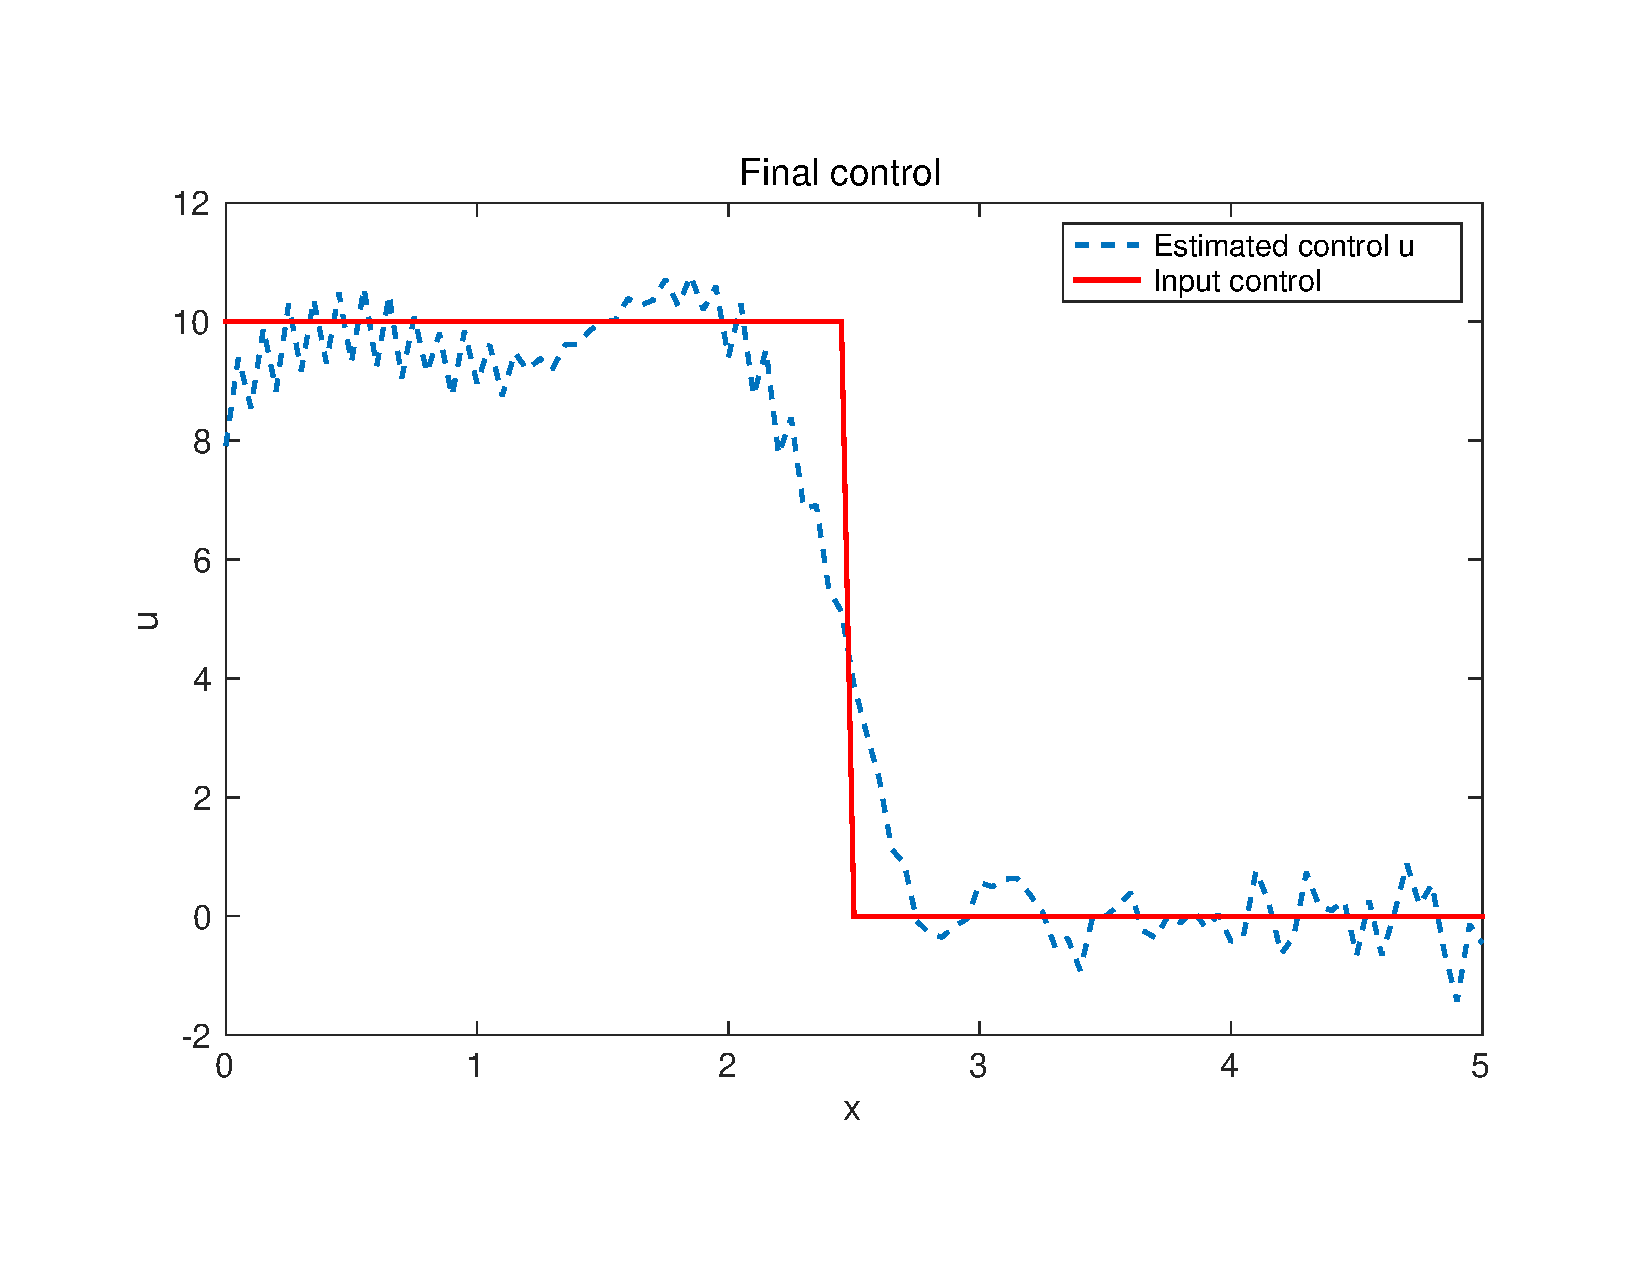
\includegraphics[width = 0.45\textwidth]{images/ex1recoveredcontrol2.pdf}
%  \caption{Recovered control for $\rg = 10^{-6}$}
%  \label{recoveredcontrol}
% \end{figure}
In \cref{recoveredstate}, the recovered state on $I\times \Omega$ and on $\{T\}\times\Omega$ is depicted. We have a quite good tracking of $y^\dag(T)$.
\begin{figure}[htb]
\centering
\subfloat{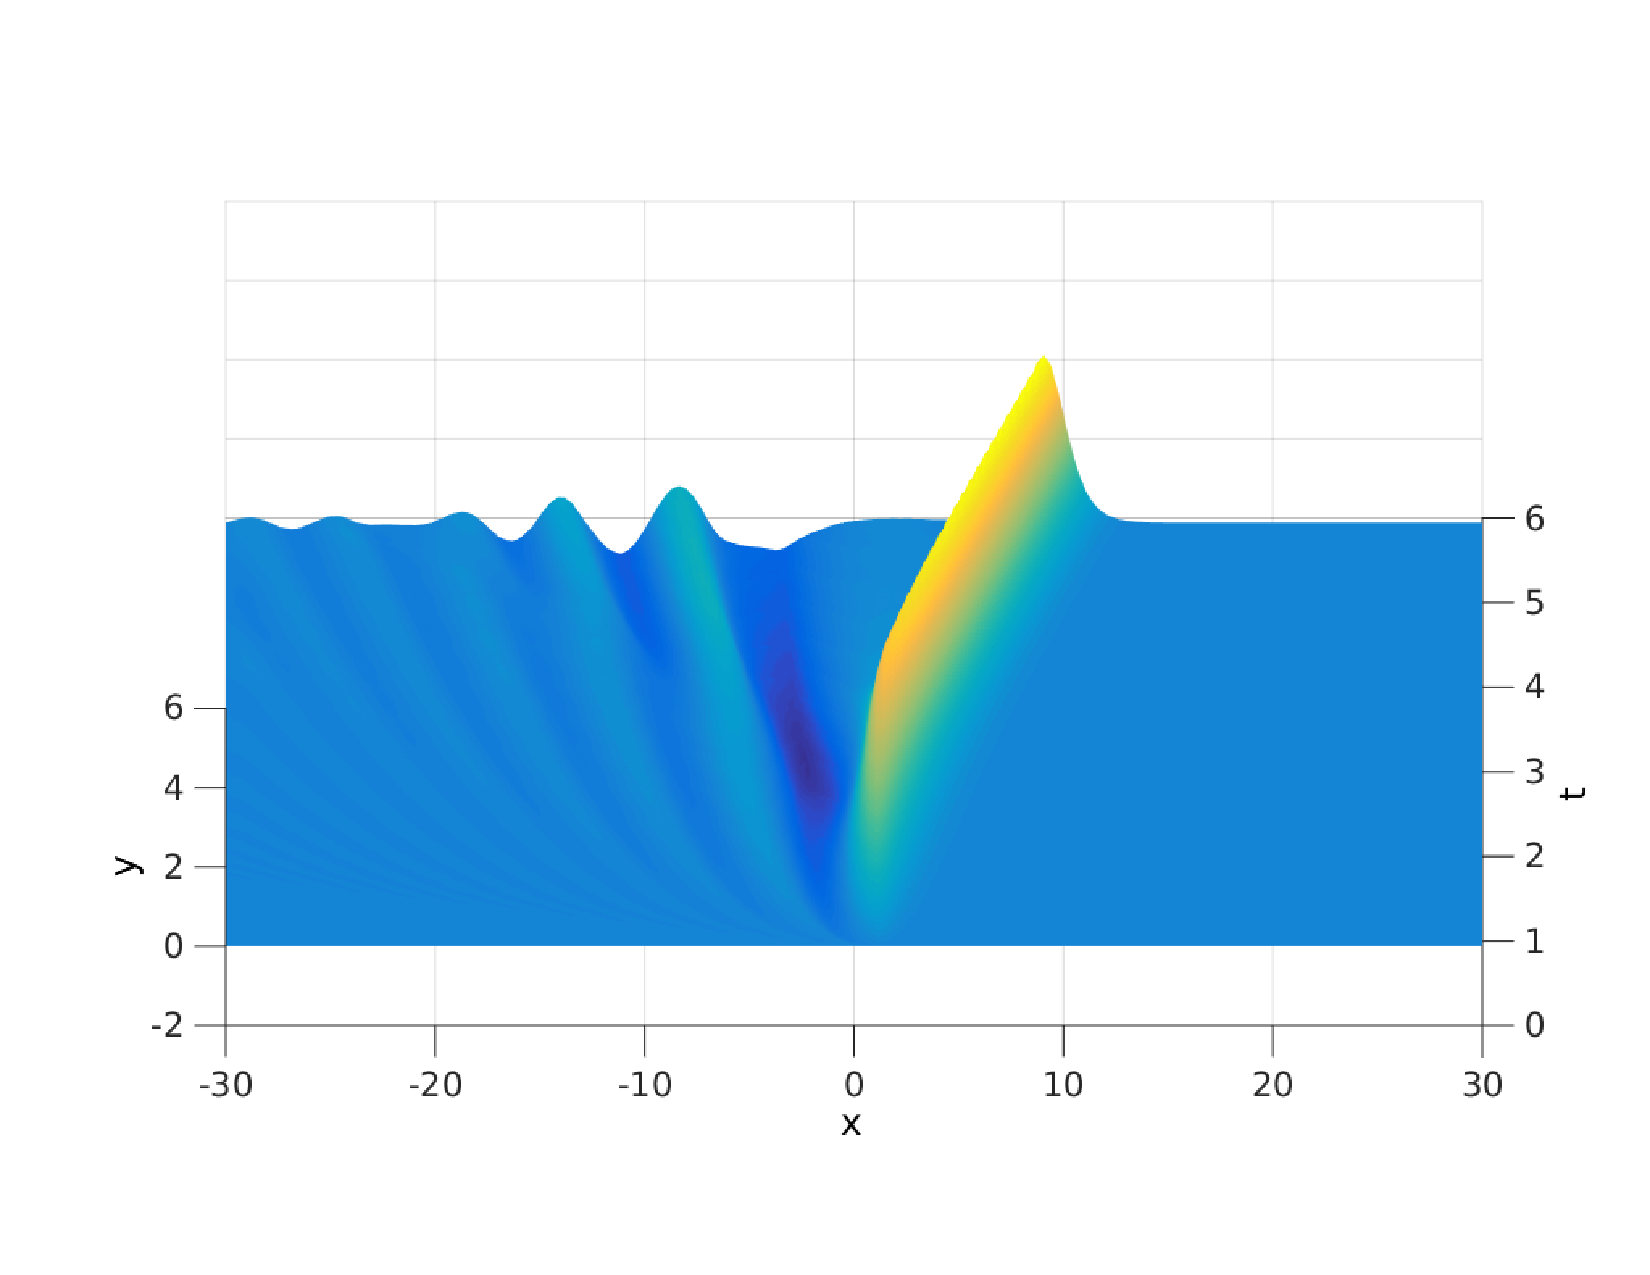
\includegraphics[width =0.48\textwidth]{images/ex1recoveredstate3d.pdf}}\quad
\subfloat{% This file was created by matlab2tikz.
% Minimal pgfplots version: 1.3
%
%The latest updates can be retrieved from
%  http://www.mathworks.com/matlabcentral/fileexchange/22022-matlab2tikz
%where you can also make suggestions and rate matlab2tikz.
%
\definecolor{mycolor1}{rgb}{0.00000,0.44700,0.74100}%
\definecolor{mycolor2}{rgb}{0.85000,0.32500,0.09800}%
%
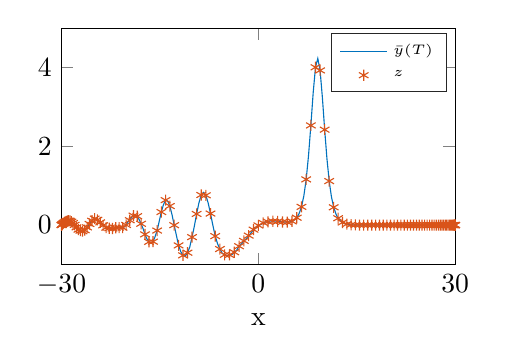
\begin{tikzpicture}

\begin{axis}[%
width=5cm,
height=3cm,
at={(0.0in,0.0in)},
scale only axis,
xmin=-30,
xmax=30,
xlabel={x},
xtick={-30,0,30},
ymin=-1,
ymax=5,
legend style={legend cell align=left,align=left,draw=white!15!black}
]
\addplot [color=mycolor1,solid,width=1.0pt]
  table[row sep=crcr]{%
-30	2.7750200095766e-16\\
-29.9977410551743	0.000394019063017496\\
-29.9909645608861	0.00142064870904568\\
-29.9796715376505	0.00335088500103346\\
-29.9638636861552	0.00579232662745137\\
-29.9435433870045	0.00923418716857076\\
-29.9187137003607	0.0130917118514944\\
-29.8893783654833	0.0180195088159707\\
-29.8555418001659	0.0232476890449561\\
-29.8172091000707	0.029573682660531\\
-29.7743860379613	0.0360275162240514\\
-29.7270790628334	0.0435224641418916\\
-29.6752952989434	0.0508641325192396\\
-29.6190425447357	0.0590531179748655\\
-29.5583292716682	0.066674122320775\\
-29.4931646229365	0.0748193715017893\\
-29.4235584120969	0.0819306215498546\\
-29.3495211215888	0.0892153258177046\\
-29.2710639011559	0.09507517837535\\
-29.1881985661668	0.100775175736473\\
-29.1009375958363	0.104778283294831\\
-29.0092941313456	0.108295444432115\\
-28.9132819738632	0.109879924891737\\
-28.812915582467	0.110057872038979\\
-28.7082100719663	0.106744338343567\\
-28.5991812106258	0.0991297866496285\\
-28.4858454177911	0.0861208114302304\\
-28.3682197614156	0.069111950868396\\
-28.2463219554906	0.0505156662273659\\
-28.1201703573772	0.0299057893789364\\
-27.9897839650422	0.00558486377014525\\
-27.8551824141965	-0.0252121911973948\\
-27.7163859753386	-0.0573824719332141\\
-27.5734155507017	-0.0883747412698683\\
-27.4262926711059	-0.115933296987125\\
-27.2750394927157	-0.129338973841541\\
-27.1196787937033	-0.142616632734754\\
-26.9602339708186	-0.152902351642472\\
-26.7967290358655	-0.155944935774009\\
-26.6291886120856	-0.152008516500226\\
-26.4576379304506	-0.129793034157218\\
-26.2821028258622	-0.0974690039529611\\
-26.1026097332613	-0.0585560184781467\\
-25.9191856836476	-0.0146056861584369\\
-25.7318583000082	0.0276207468750323\\
-25.540655793158	0.0709005212967846\\
-25.3456069574912	0.109606452562699\\
-25.1467411666451	0.145574588584855\\
-24.9440883690764	0.163663819696391\\
-24.7376790835508	0.156763333069087\\
-24.5275443945475	0.132800272082066\\
-24.3137159475778	0.109442570358179\\
-24.0962259444193	0.0675611793464422\\
-23.8751071382665	0.0224534609575968\\
-23.6503928287982	-0.0065273500406641\\
-23.4221168571628	-0.0270161273060217\\
-23.1903136008821	-0.0658050174524026\\
-22.9550179686738	-0.0830557609078522\\
-22.7162653951945	-0.0801575002632708\\
-22.4740918357038	-0.079496021490671\\
-22.2285337606488	-0.0866979906492435\\
-21.9796281501724	-0.0756748935867256\\
-21.727412488544	-0.0687026265574736\\
-21.4719247585146	-0.062364554895804\\
-21.2132034355964	-0.0636281631666539\\
-20.9512874822692	-0.0701331453985469\\
-20.686216342112	-0.0650226797019239\\
-20.4180299338636	-0.0450237520061837\\
-20.1467686454106	0.00245576253533866\\
-19.8724733277052	0.0778822910453666\\
-19.5951852886133	0.12325161135821\\
-19.3149462866937	0.194135053868776\\
-19.0317985249094	0.239399787856684\\
-18.7457846442716	0.251804515020571\\
-18.4569477174188	0.225580833606365\\
-18.1653312421298	0.139420005722202\\
-17.870979134773	0.0326811309954234\\
-17.5739357236932	-0.0874175320941998\\
-17.2742457425354	-0.236663182445218\\
-16.9719543235084	-0.353130405277066\\
-16.6671069905881	-0.426509358938161\\
-16.3597496526614	-0.459357080009697\\
-16.0499285966129	-0.421457871113608\\
-15.7376904803541	-0.29525171183373\\
-15.4230823257966	-0.139203439979348\\
-15.1061515117715	0.097216300480885\\
-14.7869457668935	0.331432330259947\\
-14.4655131623737	0.516920777793631\\
-14.1419021047799	0.633631146764418\\
-13.8161613287472	0.611094704347243\\
-13.4883398896382	0.483129238126205\\
-13.1584871561558	0.265653025892191\\
-12.8266528029085	-0.0027543679205839\\
-12.4928868029291	-0.259726597017288\\
-12.1572394201497	-0.516346534514419\\
-11.8197612018314	-0.676187407488916\\
-11.4805029709527	-0.769038404991656\\
-11.1395158185551	-0.790344571054461\\
-10.7968510960496	-0.702234185804902\\
-10.452560407483	-0.556928147013625\\
-10.1066956017666	-0.306163473032411\\
-9.75930876486789	-0.0332490264828111\\
-9.41045221196674	0.282644278872761\\
-9.06017847957684	0.561335642237514\\
-8.70854031763387	0.764171791051455\\
-8.35559068155159	0.828099938395791\\
-8.00138272424695	0.756269862642633\\
-7.64596978813544	0.560431038988892\\
-7.28940539709792	0.292424466005655\\
-6.93174324842013	-0.00498543892155733\\
-6.57303720470609	-0.280398860523595\\
-6.21334128576655	-0.475029207362736\\
-5.85270966048385	-0.608822087771285\\
-5.49119663865423	-0.719711079384843\\
-5.12885666280904	-0.755103800557331\\
-4.76574430001584	-0.778772546751816\\
-4.40191423366085	-0.757850154244603\\
-4.03742125521378	-0.753325032452601\\
-3.67232025597648	-0.689994801009742\\
-3.30666621881649	-0.640057783401391\\
-2.94051420988682	-0.537452517964341\\
-2.57391937033319	-0.482619108960294\\
-2.20693690799002	-0.401627667491827\\
-1.83962208906626	-0.347029048467091\\
-1.47203022982254	-0.26765762411631\\
-1.10421668824077	-0.195290556771989\\
-0.736236855687364	-0.116717101858913\\
-0.368146148571595	-0.0687783241056578\\
1.83697019872103e-15	-0.00876395576861893\\
0.368146148571598	0.0108469422536653\\
0.736236855687368	0.0557884877550458\\
1.10421668824077	0.0773789704041557\\
1.47203022982254	0.0832277316195522\\
1.83962208906626	0.106717634742993\\
2.20693690799002	0.0973005589430964\\
2.5739193703332	0.104998871277038\\
2.94051420988682	0.0913542759277906\\
3.3066662188165	0.0916014838037763\\
3.67232025597649	0.0788264678419476\\
4.03742125521379	0.0789856142995589\\
4.40191423366085	0.0730950785302203\\
4.76574430001584	0.0820426102610695\\
5.12885666280904	0.094132489168005\\
5.49119663865423	0.129526795265583\\
5.85270966048385	0.186749170262569\\
6.21334128576656	0.292439596730601\\
6.57303720470609	0.462672203701685\\
6.93174324842014	0.740130425689453\\
7.28940539709792	1.16037167627275\\
7.64596978813544	1.76293964783716\\
8.00138272424695	2.53101817958062\\
8.35559068155159	3.35747869470354\\
8.70854031763387	4.00818493022126\\
9.06017847957685	4.23202552229897\\
9.41045221196675	3.9276898964992\\
9.75930876486789	3.23954616365804\\
10.1066956017666	2.42290275101356\\
10.452560407483	1.6875796284398\\
10.7968510960496	1.11755047210551\\
11.1395158185551	0.718272057415781\\
11.4805029709527	0.451593019877358\\
11.8197612018314	0.281827733595218\\
12.1572394201497	0.173711663232523\\
12.4928868029291	0.10766969099577\\
12.8266528029085	0.0656644764794021\\
13.1584871561558	0.0408352487656479\\
13.4883398896382	0.024498742804448\\
13.8161613287472	0.01539330704019\\
14.1419021047799	0.008851306330871\\
14.4655131623737	0.00568041772554212\\
14.7869457668935	0.00289225752692578\\
15.1061515117715	0.00195337819328063\\
15.4230823257966	0.000628831130455375\\
15.7376904803541	0.00052125371735116\\
16.0499285966129	-0.000214468624407908\\
16.3597496526614	-2.31645267710164e-05\\
16.6671069905881	-0.000508803174393548\\
16.9719543235084	-0.000221634343849239\\
17.2742457425354	-0.000591009917137941\\
17.5739357236932	-0.000284973557003246\\
17.870979134773	-0.000592547151569827\\
18.1653312421298	-0.000296063385913437\\
18.4569477174188	-0.00056505036645249\\
18.7457846442716	-0.000287714949574674\\
19.0317985249094	-0.000528817188324081\\
19.3149462866937	-0.000272908861660111\\
19.5951852886133	-0.000491699596901352\\
19.8724733277052	-0.000256741992792963\\
20.1467686454106	-0.000456539352617016\\
20.4180299338636	-0.000241154754076958\\
20.686216342112	-0.000424214411733437\\
20.9512874822692	-0.000226771907531674\\
21.2132034355964	-0.000394857889115585\\
21.4719247585146	-0.000213720809519349\\
21.727412488544	-0.000368290193514579\\
21.9796281501724	-0.00020195232643032\\
22.2285337606488	-0.000344262458814857\\
22.4740918357038	-0.00019133507588647\\
22.7162653951945	-0.0003225034955488\\
22.9550179686738	-0.000181764407333634\\
23.1903136008821	-0.000302741382225174\\
23.4221168571628	-0.000173108574476454\\
23.6503928287982	-0.000284787787391498\\
23.8751071382665	-0.000165245448006778\\
24.0962259444193	-0.00026841123311958\\
24.3137159475778	-0.000158123907238824\\
24.5275443945475	-0.000253441221740969\\
24.7376790835508	-0.000151624461869008\\
24.9440883690764	-0.000239738553864647\\
25.1467411666451	-0.000145709908459832\\
25.3456069574912	-0.000227144115607009\\
25.540655793158	-0.000140299722216856\\
25.7318583000082	-0.000215557251881435\\
25.9191856836476	-0.000135361746359292\\
26.1026097332613	-0.000204843911935303\\
26.2821028258622	-0.000130832778573269\\
26.4576379304507	-0.000194920654439751\\
26.6291886120856	-0.000126679951151403\\
26.7967290358655	-0.000185681349751592\\
26.9602339708186	-0.00012282963272981\\
27.1196787937033	-0.000177019442541396\\
27.2750394927157	-0.000119223574370299\\
27.4262926711059	-0.000168789698183386\\
27.5734155507017	-0.000115681081147803\\
27.7163859753386	-0.000160704343402889\\
27.8551824141965	-0.00011184414307855\\
27.9897839650422	-0.000152248190470157\\
28.1201703573772	-0.000107052651245434\\
28.2463219554906	-0.000142553932134539\\
28.3682197614156	-0.000100329965976034\\
28.4858454177911	-0.000130605649224817\\
28.5991812106258	-9.07659346860412e-05\\
28.7082100719663	-0.000115709944811938\\
28.812915582467	-7.80372592582292e-05\\
28.9132819738632	-9.80006086017054e-05\\
29.0092941313456	-6.27964067077929e-05\\
29.1009375958363	-7.86284324535816e-05\\
29.1881985661668	-4.66037538142962e-05\\
29.2710639011559	-5.94105163046762e-05\\
29.3495211215888	-3.13520091089985e-05\\
29.4235584120969	-4.21461935609946e-05\\
29.4931646229365	-1.85969339865097e-05\\
29.5583292716682	-2.80506076260601e-05\\
29.6190425447358	-9.15171613480416e-06\\
29.6752952989434	-1.75367070515178e-05\\
29.7270790628334	-3.05266428809208e-06\\
29.7743860379613	-1.03339990572206e-05\\
29.8172091000707	2.20380042199122e-07\\
29.8555418001659	-5.7690398994189e-06\\
29.8893783654833	1.44969338098646e-06\\
29.9187137003607	-3.05202295716094e-06\\
29.9435433870045	1.43675748324689e-06\\
29.9638636861552	-1.47923579161816e-06\\
29.9796715376505	8.609469918271e-07\\
29.9909645608861	-5.44640285984394e-07\\
29.9977410551743	2.26981706122406e-07\\
30	0\\
};
\addlegendentry{\tiny$\bar y(T)$};

\addplot [color=mycolor2,only marks,mark=asterisk,mark options={solid}]
  table[row sep=crcr]{%
-30	2.7750200095766e-16\\
-29.9909645608861	0.00142064870904568\\
-29.9638636861552	0.00579232662745137\\
-29.9187137003607	0.0130917118514944\\
-29.8555418001659	0.0232476890449561\\
-29.7743860379613	0.0360275162240514\\
-29.6752952989434	0.0508641325192396\\
-29.5583292716682	0.066674122320775\\
-29.4235584120969	0.0819306215498546\\
-29.2710639011559	0.09507517837535\\
-29.1009375958363	0.104778283294831\\
-28.9132819738632	0.109879924891737\\
-28.7082100719663	0.106744338343567\\
-28.4858454177911	0.0861208114302304\\
-28.2463219554906	0.0505156662273659\\
-27.9897839650422	0.00558486377014525\\
-27.7163859753386	-0.0573824719332141\\
-27.4262926711059	-0.115933296987125\\
-27.1196787937033	-0.142616632734754\\
-26.7967290358655	-0.155944935774009\\
-26.4576379304506	-0.129793034157218\\
-26.1026097332613	-0.0585560184781467\\
-25.7318583000082	0.0276207468750323\\
-25.3456069574912	0.109606452562699\\
-24.9440883690764	0.163663819696391\\
-24.5275443945475	0.132800272082066\\
-24.0962259444193	0.0675611793464422\\
-23.6503928287982	-0.0065273500406641\\
-23.1903136008821	-0.0658050174524026\\
-22.7162653951945	-0.0801575002632708\\
-22.2285337606488	-0.0866979906492435\\
-21.727412488544	-0.0687026265574736\\
-21.2132034355964	-0.0636281631666539\\
-20.686216342112	-0.0650226797019239\\
-20.1467686454106	0.00245576253533866\\
-19.5951852886133	0.12325161135821\\
-19.0317985249094	0.239399787856684\\
-18.4569477174188	0.225580833606365\\
-17.870979134773	0.0326811309954234\\
-17.2742457425354	-0.236663182445218\\
-16.6671069905881	-0.426509358938161\\
-16.0499285966129	-0.421457871113608\\
-15.4230823257966	-0.139203439979348\\
-14.7869457668935	0.331432330259947\\
-14.1419021047799	0.633631146764418\\
-13.4883398896382	0.483129238126205\\
-12.8266528029085	-0.0027543679205839\\
-12.1572394201497	-0.516346534514419\\
-11.4805029709527	-0.769038404991656\\
-10.7968510960496	-0.702234185804902\\
-10.1066956017666	-0.306163473032411\\
-9.41045221196674	0.282644278872761\\
-8.70854031763387	0.764171791051455\\
-8.00138272424695	0.756269862642633\\
-7.28940539709792	0.292424466005655\\
-6.57303720470609	-0.280398860523595\\
-5.85270966048385	-0.608822087771285\\
-5.12885666280904	-0.755103800557331\\
-4.40191423366085	-0.757850154244603\\
-3.67232025597648	-0.689994801009742\\
-2.94051420988682	-0.537452517964341\\
-2.20693690799002	-0.401627667491827\\
-1.47203022982254	-0.26765762411631\\
-0.736236855687364	-0.116717101858913\\
1.83697019872103e-15	-0.00876395576861893\\
0.736236855687368	0.0557884877550458\\
1.47203022982254	0.0832277316195522\\
2.20693690799002	0.0973005589430964\\
2.94051420988682	0.0913542759277906\\
3.67232025597649	0.0788264678419476\\
4.40191423366085	0.0730950785302203\\
5.12885666280904	0.094132489168005\\
5.85270966048385	0.186749170262569\\
6.57303720470609	0.462672203701685\\
7.28940539709792	1.16037167627275\\
8.00138272424695	2.53101817958062\\
8.70854031763387	4.00818493022126\\
9.41045221196675	3.9276898964992\\
10.1066956017666	2.42290275101356\\
10.7968510960496	1.11755047210551\\
11.4805029709527	0.451593019877358\\
12.1572394201497	0.173711663232523\\
12.8266528029085	0.0656644764794021\\
13.4883398896382	0.024498742804448\\
14.1419021047799	0.008851306330871\\
14.7869457668935	0.00289225752692578\\
15.4230823257966	0.000628831130455375\\
16.0499285966129	-0.000214468624407908\\
16.6671069905881	-0.000508803174393548\\
17.2742457425354	-0.000591009917137941\\
17.870979134773	-0.000592547151569827\\
18.4569477174188	-0.00056505036645249\\
19.0317985249094	-0.000528817188324081\\
19.5951852886133	-0.000491699596901352\\
20.1467686454106	-0.000456539352617016\\
20.686216342112	-0.000424214411733437\\
21.2132034355964	-0.000394857889115585\\
21.727412488544	-0.000368290193514579\\
22.2285337606488	-0.000344262458814857\\
22.7162653951945	-0.0003225034955488\\
23.1903136008821	-0.000302741382225174\\
23.6503928287982	-0.000284787787391498\\
24.0962259444193	-0.00026841123311958\\
24.5275443945475	-0.000253441221740969\\
24.9440883690764	-0.000239738553864647\\
25.3456069574912	-0.000227144115607009\\
25.7318583000082	-0.000215557251881435\\
26.1026097332613	-0.000204843911935303\\
26.4576379304507	-0.000194920654439751\\
26.7967290358655	-0.000185681349751592\\
27.1196787937033	-0.000177019442541396\\
27.4262926711059	-0.000168789698183386\\
27.7163859753386	-0.000160704343402889\\
27.9897839650422	-0.000152248190470157\\
28.2463219554906	-0.000142553932134539\\
28.4858454177911	-0.000130605649224817\\
28.7082100719663	-0.000115709944811938\\
28.9132819738632	-9.80006086017054e-05\\
29.1009375958363	-7.86284324535816e-05\\
29.2710639011559	-5.94105163046762e-05\\
29.4235584120969	-4.21461935609946e-05\\
29.5583292716682	-2.80506076260601e-05\\
29.6752952989434	-1.75367070515178e-05\\
29.7743860379613	-1.03339990572206e-05\\
29.8555418001659	-5.7690398994189e-06\\
29.9187137003607	-3.05202295716094e-06\\
29.9638636861552	-1.47923579161816e-06\\
29.9909645608861	-5.44640285984394e-07\\
30	0\\
};
\addlegendentry{\tiny $z$};

\end{axis}
\end{tikzpicture}%}
\caption{Recovered state $\bar y$ and terminal state $\bar y(T)$}
\label{recoveredstate}
\end{figure}

\paragraph{\underline{Control example}}
 The second example is a control example which is concerned with the optimal placement of bumps on the bottom of a narrow channel for the generation of a desired flow. We divide the domain $\Omega = [-L,L]$, $L=30$ into two subdomains. The domain $\Omega_c = [-L,0]$ is the control domain, while $\Omega_{o} = [0,L]$ is the observation domain, see \cref{controlsetup} for the description of the setup. The flow enters the domain from the right and we want to create the flow profile $z$ shown in \cref{controlsetup} on $\Omega_{o}$ at final time $T$, acting only on $\Omega_c$. Here the space-time grid is parametrized with $N = 512$ spatial grid points and a time-step size of $\Delta t = 0.01$.
\begin{figure}[htb]
\centering
\subfloat{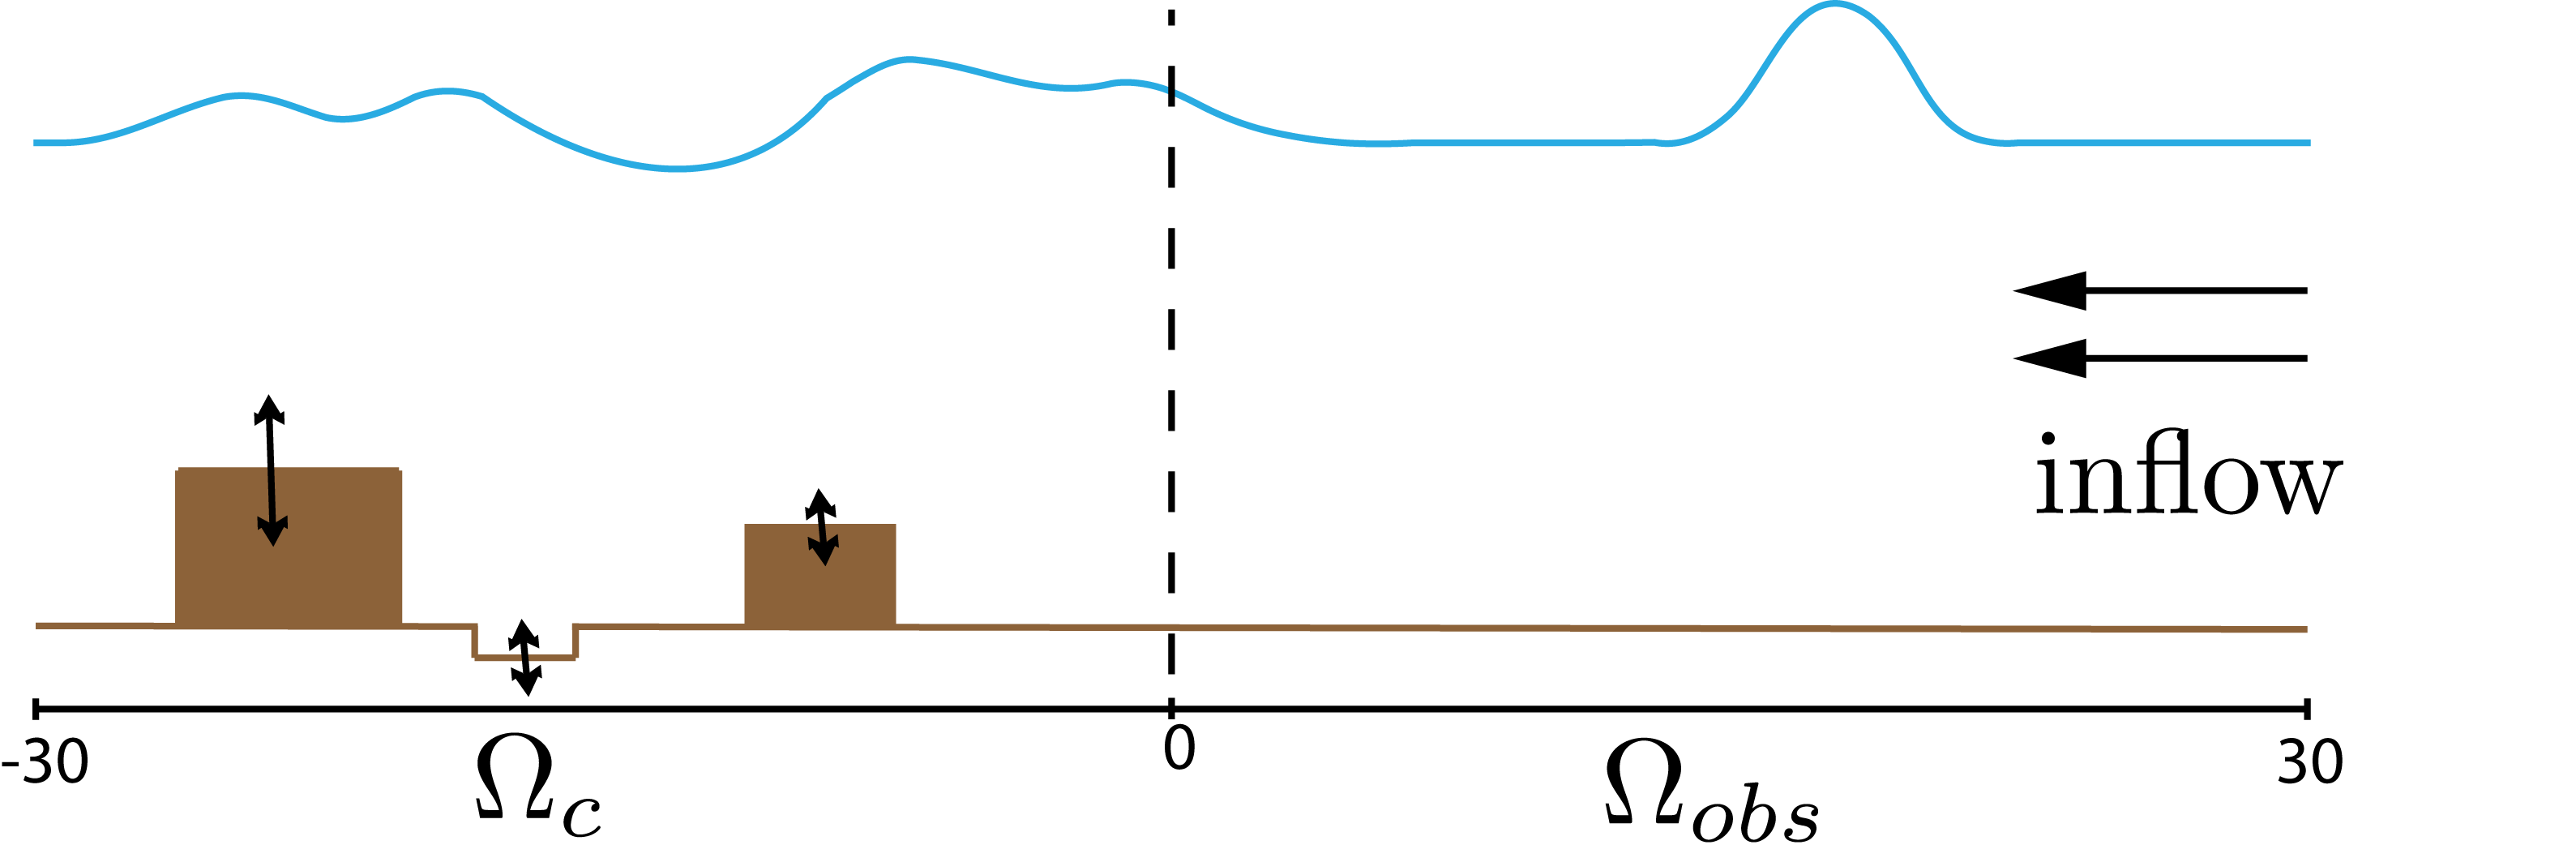
\includegraphics[width=0.48\textwidth, height=3cm]{images/control_setup.png}}\quad
\subfloat{% This file was created by matlab2tikz.
% Minimal pgfplots version: 1.3
%
%The latest updates can be retrieved from
%  http://www.mathworks.com/matlabcentral/fileexchange/22022-matlab2tikz
%where you can also make suggestions and rate matlab2tikz.
%
\definecolor{mycolor1}{rgb}{0.00000,0.44700,0.74100}%
%
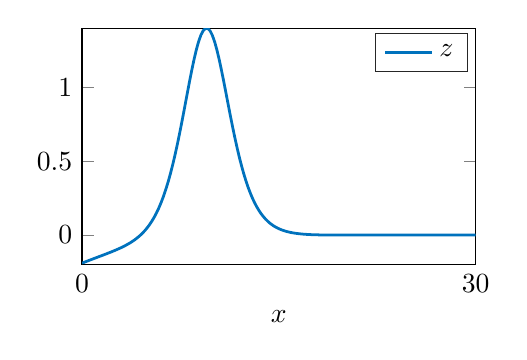
\begin{tikzpicture}

\begin{axis}[%
width=5cm,
height=3cm,
at={(0.0in,0.0in)},
scale only axis,
xmin=0,
xmax=30,
xlabel={$x$},
xtick={0,30},
ymin=-0.2,
ymax=1.4,
legend style={legend cell align=left,align=left,draw=white!15!black}
]
\addplot [color=mycolor1,solid,line width=1.0pt]
  table[row sep=crcr]{%
1.83697019872103e-15	-0.19107600324811\\
0.184076539474635	-0.184665296965219\\
0.368146148571598	-0.178359462325261\\
0.552201897174145	-0.172015592007278\\
0.736236855687368	-0.165858954505256\\
0.920244095299097	-0.159554664608493\\
1.10421668824077	-0.153495229137086\\
1.28814770804823	-0.1471858142788\\
1.47203022982254	-0.141155367547741\\
1.6558573304907	-0.134773981736065\\
1.83962208906626	-0.128681586113806\\
2.02331758690992	-0.122132616492776\\
2.20693690799002	-0.115856214495644\\
2.3904731391429	-0.109006263025219\\
2.5739193703332	-0.102381793024638\\
2.75726869491398	-0.0950477043319437\\
2.94051420988682	-0.0878550670217143\\
3.12364901616164	-0.0797883768524927\\
3.3066662188165	-0.0717335887095961\\
3.48955892735715	-0.0626008125183623\\
3.67232025597649	-0.0532938314873238\\
3.8549433238138	-0.0426522801941074\\
4.03742125521379	-0.0315804518144613\\
4.21974717998548	-0.0188499714398536\\
4.40191423366085	-0.00534809514411409\\
4.5839155577533	0.0102193723048755\\
4.76574430001584	0.0269992666685855\\
4.9473936146991	0.0463475694533376\\
5.12885666280904	0.0674598795267957\\
5.31012661236447	0.0917443578113549\\
5.49119663865423	0.118453919119807\\
5.67205992449419	0.149027577567872\\
5.85270966048385	0.182771668354493\\
6.03313904526276	0.2211137425042\\
6.21334128576656	0.263387924764477\\
6.39330959748274	0.310934753160446\\
6.57303720470609	0.363057638505416\\
6.75251734079378	0.420888685306625\\
6.93174324842014	0.483600720136107\\
7.11070817983102	0.551944418209389\\
7.28940539709792	0.624825032353612\\
7.46782817237161	0.702402260090318\\
7.64596978813544	0.783172265776814\\
7.82382353745827	0.866510710752312\\
8.00138272424695	0.950432918374239\\
8.17864066349847	1.033452021175\\
8.35559068155159	1.11320758852322\\
8.53222611633815	1.18750136314383\\
8.70854031763387	1.25396439421819\\
8.88452664730872	1.31012182434346\\
9.06017847957685	1.35419611761404\\
9.23548920124605	1.38405577389348\\
9.41045221196675	1.39914426423522\\
9.58506092448047	1.3982199566102\\
9.75930876486789	1.38230384180084\\
9.93318917279629	1.35124070364233\\
10.1066956017666	1.30751039934605\\
10.2798215193598	1.2517989212938\\
10.452560407483	1.1875076554457\\
10.6249057626147	1.11563859089642\\
10.7968510960496	1.03982782266806\\
10.9683899341432	0.960868494234491\\
11.1395158185551	0.882077386034359\\
11.3102223064926	0.803718052244273\\
11.4805029709527	0.728502655144989\\
11.6503514009648	0.656090636174479\\
11.8197612018314	0.588549719196727\\
11.9887259953694	0.525033292775272\\
12.1572394201497	0.467069798990587\\
12.3252951317371	0.413475266799522\\
12.4928868029291	0.365391340461634\\
12.660008123994	0.321461551994615\\
12.8266528029085	0.28258068514618\\
12.9928145655946	0.247346034625388\\
13.1584871561558	0.216509622419505\\
13.3236643371129	0.188704053245488\\
13.4883398896382	0.164605776294786\\
13.6525076137903	0.142927266132262\\
13.8161613287472	0.124307745912919\\
13.979294873039	0.107558453953097\\
14.1419021047799	0.0933004144897742\\
14.3039769018997	0.0804468747255456\\
14.4655131623737	0.069608159222147\\
14.6265048044531	0.059794364415901\\
14.7869457668935	0.05160647415781\\
14.9468300091835	0.0441425048358034\\
15.1061515117715	0.0379926438255384\\
15.2649042762932	0.0323328174560626\\
15.4230823257966	0.027740023404666\\
15.5806797049677	0.0234584082012918\\
15.7376904803541	0.0200494033898582\\
15.8941087405888	0.0168166436553419\\
16.0499285966129	0.0143040473264534\\
16.2051441818968	0.0118671648816153\\
16.3597496526614	0.0100310136260494\\
16.5137391880981	0.00819663010382607\\
16.6671069905881	0.00686928079451349\\
16.8198472859201	0.00549009091511992\\
16.9719543235084	0.0045441883982762\\
17.123422376609	0.00350827021782924\\
17.2742457425354	0.00284730809641459\\
17.4244187428729	0.00206979063455761\\
17.5739357236932	0.00162079232101538\\
17.7227910557662	0.00103741686398575\\
17.870979134773	0.000745302894166253\\
18.0184943815161	0.000307483702400596\\
18.1653312421298	0.000130759791860469\\
18.3114841882893	-0.000198193108109003\\
18.4569477174188	-0.000290722734136554\\
18.6017163528987	-0.000538478199195395\\
18.7457846442716	-0.00057021570408132\\
18.8891471674478	-0.0007576080252716\\
19.0317985249094	-0.000746057751602231\\
19.1737333459133	-0.000888751137929062\\
19.3149462866937	-0.00084696272144762\\
19.4554320306634	-0.000956705494223572\\
19.5951852886133	-0.000894369219002267\\
19.7342007989124	-0.00097995334911576\\
19.8724733277052	-0.000904222198064241\\
20.0099976691091	-0.000972208254679084\\
20.1467686454106	-0.000888329883630556\\
20.2827811072595	-0.000943591760590768\\
20.4180299338636	-0.000855382403952933\\
20.552510033181	-0.000901526783467936\\
20.686216342112	-0.000811728180256484\\
20.8191438266896	-0.000851409567250059\\
20.9512874822692	-0.000761961505860465\\
21.0826423337168	-0.000797118092342516\\
21.2132034355964	-0.000709367026910097\\
21.3429658723565	-0.000741400751120002\\
21.4719247585146	-0.000656248325031653\\
21.6000752388414	-0.000686167552271355\\
21.727412488544	-0.000604190328605039\\
21.8539317134468	-0.000632700821665998\\
21.9796281501724	-0.000554242964154504\\
22.1044970663211	-0.00058183578466837\\
22.2285337606488	-0.000507061162927481\\
22.351733563244	-0.000534067878309244\\
22.4740918357038	-0.000463025917715953\\
22.5956039713084	-0.000489654682896844\\
22.7162653951945	-0.000422304154165534\\
22.8360715645279	-0.000448686894093682\\
22.9550179686738	-0.000384927323903202\\
23.0731001293674	-0.000411128217258295\\
23.1903136008821	-0.000350823659854815\\
23.306653970197	-0.000376868856645403\\
23.4221168571628	-0.000319854883119753\\
23.5366979146673	-0.000345739505669752\\
23.6503928287982	-0.000291841181839992\\
23.7631973190064	-0.000317542162779675\\
23.8751071382665	-0.000266577074794367\\
23.9861180732372	-0.000292057248518383\\
24.0962259444193	-0.000243844310403547\\
24.205426606314	-0.000269062910780224\\
24.3137159475778	-0.000223421939112451\\
24.4210898911785	-0.000248331365271566\\
24.5275443945475	-0.000205093643976611\\
24.6330754497331	-0.000229648696410837\\
24.7376790835508	-0.000188647110829554\\
24.8413513577327	-0.00021280369304089\\
24.9440883690764	-0.000173888133336431\\
25.0458862495914	-0.000197602626461775\\
25.1467411666451	-0.000160626725725221\\
25.246649323107	-0.000183864270454974\\
25.3456069574912	-0.00014869692275174\\
25.4436103440989	-0.000171420100758046\\
25.540655793158	-0.00013793907480218\\
25.636739650962	-0.000160122738644239\\
25.7318583000082	-0.000128215772700557\\
25.826008159133	-0.000149831353220999\\
25.9191856836476	-0.000119399541917075\\
26.0113873654708	-0.000140430977183798\\
26.1026097332613	-0.000111381012722735\\
26.1928493525487	-0.000131808230085266\\
26.2821028258622	-0.000104061482000405\\
26.370366792859	-0.00012387729120977\\
26.4576379304507	-9.73592519219394e-05\\
26.5439129529281	-0.000116549789924143\\
26.6291886120856	-9.11979053513033e-05\\
26.7134616973427	-0.000109764162500272\\
26.7967290358655	-8.55226012351301e-05\\
26.8789874926856	-0.000103455063424589\\
26.9602339708186	-8.02722639812854e-05\\
27.0404654113807	-9.75770410437277e-05\\
27.1196787937033	-7.54155071513049e-05\\
27.1978711354475	-9.20884656788129e-05\\
27.2750394927157	-7.09036221111318e-05\\
27.3511809601629	-8.69495060290491e-05\\
27.4262926711059	-6.67185092223435e-05\\
27.5003717976313	-8.21420951518764e-05\\
27.5734155507017	-6.28288498511022e-05\\
27.6454211802613	-7.76276232562402e-05\\
27.7163859753386	-5.9213542888263e-05\\
27.7863072641493	-7.33997934318196e-05\\
27.8551824141965	-5.58635635083258e-05\\
27.9230088323695	-6.94313284936049e-05\\
27.9897839650422	-5.27484229092452e-05\\
28.0555052981684	-6.57041918955652e-05\\
28.1201703573772	-4.98641297894754e-05\\
28.1837767080657	-6.22078861345529e-05\\
28.2463219554906	-4.7183834778993e-05\\
28.3078037448588	-5.89051446223311e-05\\
28.3682197614156	-4.46761426441817e-05\\
28.4275677305322	-5.57713716631778e-05\\
28.4858454177911	-4.23120873518655e-05\\
28.5430506290703	-5.27612081170438e-05\\
28.5991812106258	-4.0031969198933e-05\\
28.6542350491731	-4.98104832133588e-05\\
28.7082100719663	-3.777325026437e-05\\
28.7611042468761	-4.68563040840859e-05\\
28.812915582467	-3.54672364000498e-05\\
28.8636421280712	-4.3825771356293e-05\\
28.9132819738632	-3.30418519429905e-05\\
28.9618332509307	-4.06559378007088e-05\\
29.0092941313456	-3.04446292451023e-05\\
29.0556628282325	-3.73079590890013e-05\\
29.1009375958363	-2.76497855037129e-05\\
29.1451167295876	-3.37753457340159e-05\\
29.1881985661668	-2.46700494847776e-05\\
29.2301814835673	-3.00932301252006e-05\\
29.2710639011559	-2.15569608902061e-05\\
29.3108442797326	-2.63301377056781e-05\\
29.3495211215888	-1.83903895515504e-05\\
29.3870929705632	-2.25799332979744e-05\\
29.4235584120969	-1.52718678349054e-05\\
29.4589160732867	-1.89516399455521e-05\\
29.4931646229365	-1.23082058591031e-05\\
29.5263027716079	-1.55489643452711e-05\\
29.5583292716682	-9.59235105544111e-06\\
29.589242917338	-1.24564290576432e-05\\
29.6190425447358	-7.19520124365061e-06\\
29.6477270319225	-9.73420985216367e-06\\
29.6752952989434	-5.16105977229408e-06\\
29.7017463078689	-7.4135841719065e-06\\
29.7270790628334	-3.50453732351207e-06\\
29.751292610073	-5.4968088451873e-06\\
29.7743860379613	-2.21396636337168e-06\\
29.7963584770438	-3.96305937188005e-06\\
29.8172091000707	-1.25837381969649e-06\\
29.8369371220277	-2.77516765759007e-06\\
29.8555418001659	-5.93609825097644e-07\\
29.8730224340298	-1.88534665782374e-06\\
29.8893783654833	-1.6803889377155e-07\\
29.904608978735	-1.24101181970602e-06\\
29.9187137003607	7.17438565543935e-08\\
29.9316919993258	-7.90112761684447e-07\\
29.9435433870045	1.76395160857196e-07\\
29.9542674171988	-4.84846429450209e-07\\
29.9638636861552	1.91073924779312e-07\\
29.9723318325794	-2.83859303647534e-07\\
29.9796715376505	1.53958839971547e-07\\
29.9858825250328	-1.53611577162427e-07\\
29.9909645608861	9.5552421258141e-08\\
29.9949174538747	-6.93633929963778e-08\\
29.9977410551743	3.87410316429311e-08\\
29.999435258478	-1.63144145952522e-08\\
30	0\\
};
\addlegendentry{$z$};

\end{axis}
\end{tikzpicture}%}
\caption{Control setup and data}
\label{controlsetup}
\end{figure}
 %\begin{figure}[!h]
% 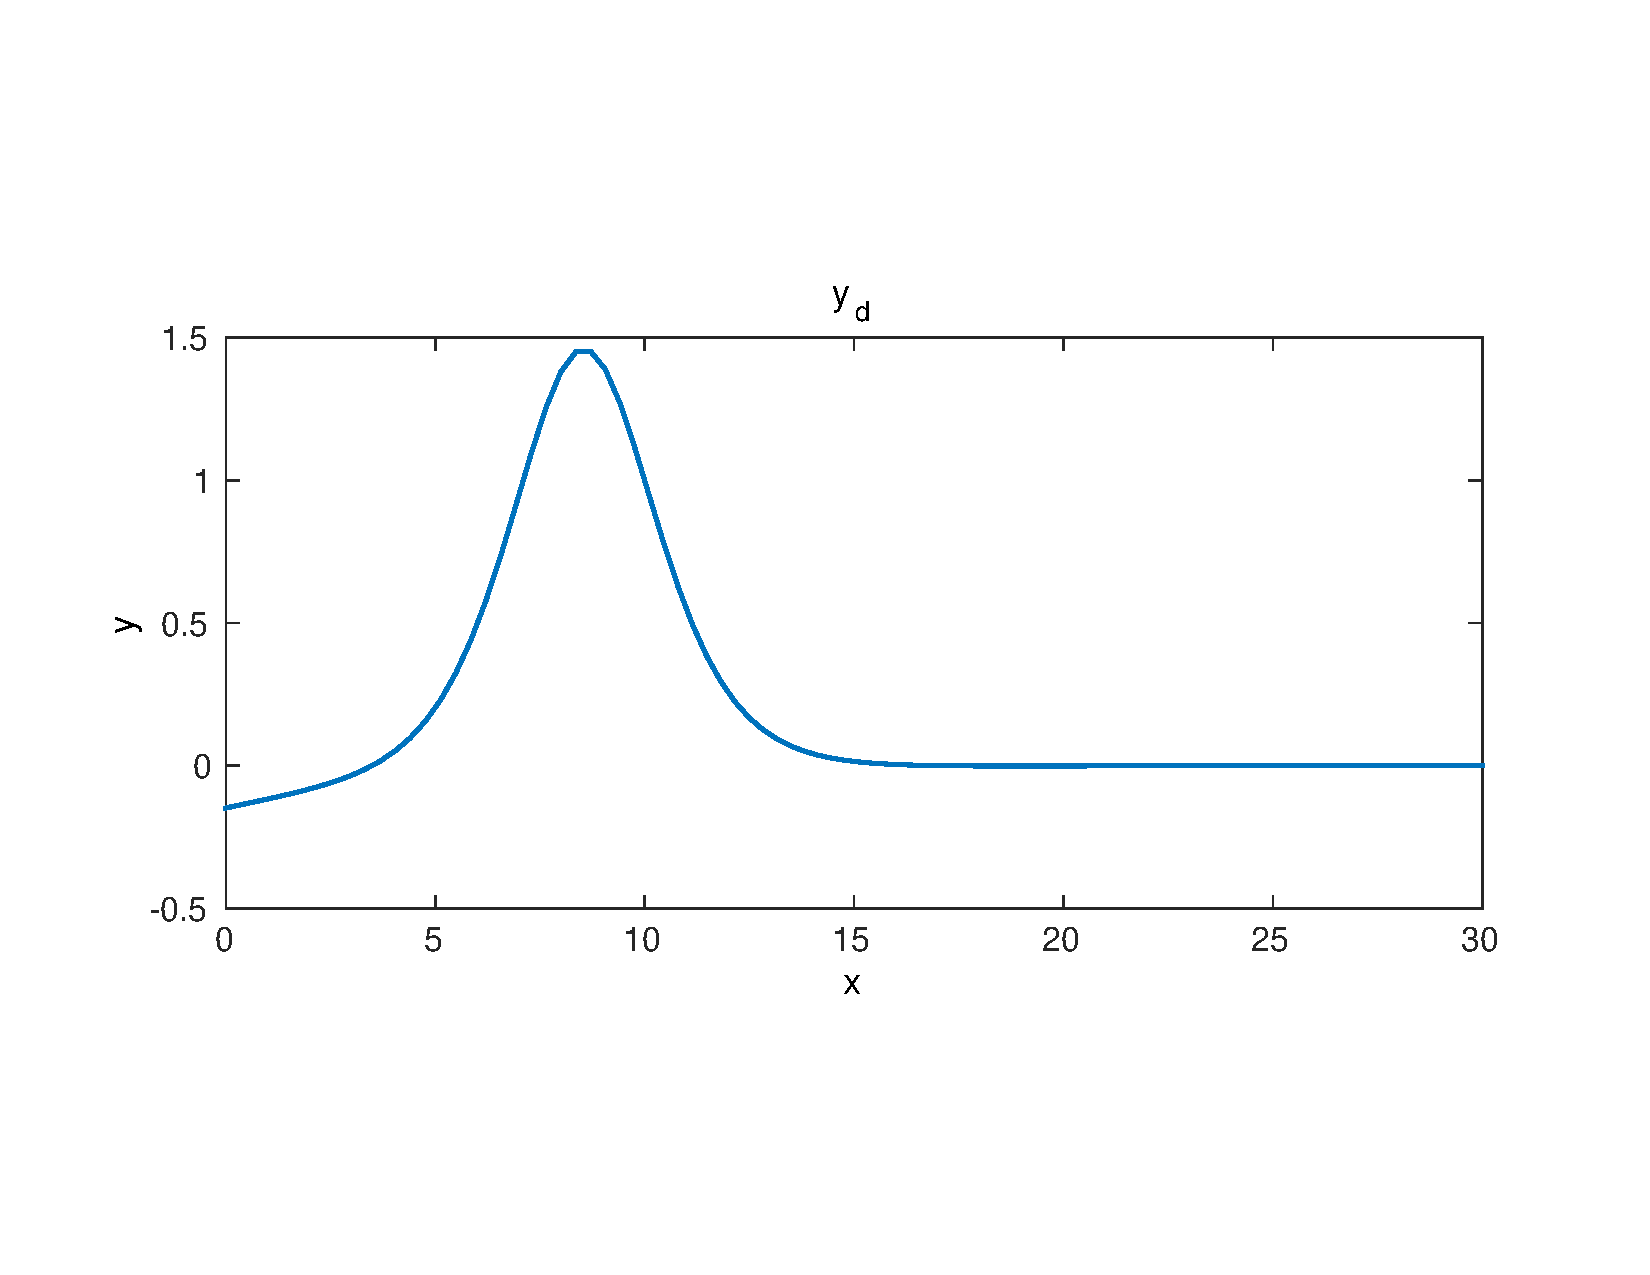
\includegraphics[width = 0.75\textwidth]{images/ex2yd.pdf}
% \caption{Objective wave at final time T.}
% \label{objectivewave}
% \end{figure}
Next, we review our numerical results. In \cref{recoveredcontrol2} the optimal control is depicted. We see that it consists of two point sources with intensities which vary smoothly in time.
\begin{figure}[htb]
\centering
\subfloat{% This file was created by matlab2tikz.
% Minimal pgfplots version: 1.3
%
%The latest updates can be retrieved from
%  http://www.mathworks.com/matlabcentral/fileexchange/22022-matlab2tikz
%where you can also make suggestions and rate matlab2tikz.
%
\begin{tikzpicture}

\begin{axis}[%
width=5cm,
height=3cm,
at={(0.0in,0.0in)},
scale only axis,
axis on top,
xmin=8.67361737988404e-19,
xmax=20,
xlabel={$t$},
ymin=-30.1171875,
ymax=30.1171875,
ylabel={$x$},
ytick={-30,0,30},
colormap={mymap}{[1pt] rgb(0pt)=(0.2081,0.1663,0.5292); rgb(1pt)=(0.211624,0.189781,0.577676); rgb(2pt)=(0.212252,0.213771,0.626971); rgb(3pt)=(0.2081,0.2386,0.677086); rgb(4pt)=(0.195905,0.264457,0.7279); rgb(5pt)=(0.170729,0.291938,0.779248); rgb(6pt)=(0.125271,0.324243,0.830271); rgb(7pt)=(0.0591333,0.359833,0.868333); rgb(8pt)=(0.0116952,0.38751,0.881957); rgb(9pt)=(0.00595714,0.408614,0.882843); rgb(10pt)=(0.0165143,0.4266,0.878633); rgb(11pt)=(0.0328524,0.443043,0.871957); rgb(12pt)=(0.0498143,0.458571,0.864057); rgb(13pt)=(0.0629333,0.47369,0.855438); rgb(14pt)=(0.0722667,0.488667,0.8467); rgb(15pt)=(0.0779429,0.503986,0.838371); rgb(16pt)=(0.0793476,0.520024,0.831181); rgb(17pt)=(0.0749429,0.537543,0.826271); rgb(18pt)=(0.0640571,0.556986,0.823957); rgb(19pt)=(0.0487714,0.577224,0.822829); rgb(20pt)=(0.0343429,0.596581,0.819852); rgb(21pt)=(0.0265,0.6137,0.8135); rgb(22pt)=(0.0238905,0.628662,0.803762); rgb(23pt)=(0.0230905,0.641786,0.791267); rgb(24pt)=(0.0227714,0.653486,0.776757); rgb(25pt)=(0.0266619,0.664195,0.760719); rgb(26pt)=(0.0383714,0.674271,0.743552); rgb(27pt)=(0.0589714,0.683757,0.725386); rgb(28pt)=(0.0843,0.692833,0.706167); rgb(29pt)=(0.113295,0.7015,0.685857); rgb(30pt)=(0.145271,0.709757,0.664629); rgb(31pt)=(0.180133,0.717657,0.642433); rgb(32pt)=(0.217829,0.725043,0.619262); rgb(33pt)=(0.258643,0.731714,0.595429); rgb(34pt)=(0.302171,0.737605,0.571186); rgb(35pt)=(0.348167,0.742433,0.547267); rgb(36pt)=(0.395257,0.7459,0.524443); rgb(37pt)=(0.44201,0.748081,0.503314); rgb(38pt)=(0.487124,0.749062,0.483976); rgb(39pt)=(0.530029,0.749114,0.466114); rgb(40pt)=(0.570857,0.748519,0.44939); rgb(41pt)=(0.609852,0.747314,0.433686); rgb(42pt)=(0.6473,0.7456,0.4188); rgb(43pt)=(0.683419,0.743476,0.404433); rgb(44pt)=(0.71841,0.741133,0.390476); rgb(45pt)=(0.752486,0.7384,0.376814); rgb(46pt)=(0.785843,0.735567,0.363271); rgb(47pt)=(0.818505,0.732733,0.34979); rgb(48pt)=(0.850657,0.7299,0.336029); rgb(49pt)=(0.882433,0.727433,0.3217); rgb(50pt)=(0.913933,0.725786,0.306276); rgb(51pt)=(0.944957,0.726114,0.288643); rgb(52pt)=(0.973895,0.731395,0.266648); rgb(53pt)=(0.993771,0.745457,0.240348); rgb(54pt)=(0.999043,0.765314,0.216414); rgb(55pt)=(0.995533,0.786057,0.196652); rgb(56pt)=(0.988,0.8066,0.179367); rgb(57pt)=(0.978857,0.827143,0.163314); rgb(58pt)=(0.9697,0.848138,0.147452); rgb(59pt)=(0.962586,0.870514,0.1309); rgb(60pt)=(0.958871,0.8949,0.113243); rgb(61pt)=(0.959824,0.921833,0.0948381); rgb(62pt)=(0.9661,0.951443,0.0755333); rgb(63pt)=(0.9763,0.9831,0.0538)},
colorbar horizontal,
colorbar style={at={(0.5,1.03)},anchor=south,xticklabel pos=upper},
point meta min=-0.225941488954968,
point meta max=1.70650395810034
]
\addplot [forget plot] graphics [xmin=8.67361737988404e-19,xmax=20,ymin=-30.1171875,ymax=30.1171875] {images/control-1.png};
\end{axis}
\end{tikzpicture}% }\quad
\subfloat{% This file was created by matlab2tikz.
% Minimal pgfplots version: 1.3
%
%The latest updates can be retrieved from
%  http://www.mathworks.com/matlabcentral/fileexchange/22022-matlab2tikz
%where you can also make suggestions and rate matlab2tikz.
%
\definecolor{mycolor1}{rgb}{0.00000,0.44700,0.74100}%
\definecolor{mycolor2}{rgb}{0.85000,0.32500,0.09800}%
%
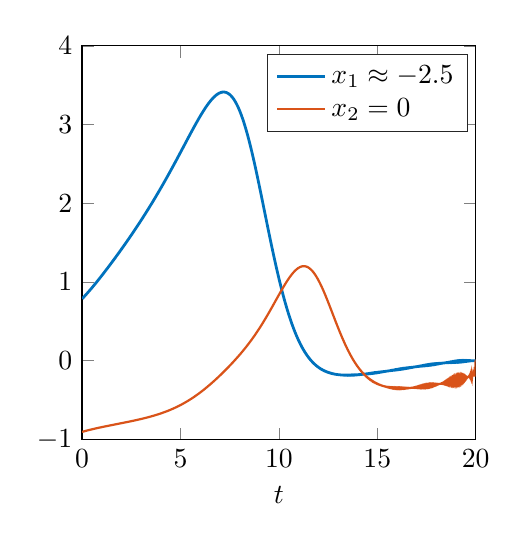
\begin{tikzpicture}

\begin{axis}[%
width=5cm,
height=5cm,
at={(0.0in,0.0in)},
scale only axis,
xmin=0,
xmax=20,
xlabel={$t$},
ymin=-1,
ymax=4.0,
legend style={legend cell align=left,align=left,draw=white!15!black}
]
\addplot [color=mycolor1,solid,line width =1.0pt]
  table[row sep=crcr]{%
0.00499750124937531	0.785941218852398\\
0.0249875062468766	0.790967202498466\\
0.0449775112443778	0.79717107427834\\
0.0649675162418791	0.802136041502122\\
0.0849575212393803	0.808371894503364\\
0.104947526236882	0.813331981225837\\
0.124937531234383	0.819642008152595\\
0.144927536231884	0.824572822071254\\
0.164917541229385	0.830805611336683\\
0.184907546226887	0.835624620104127\\
0.204897551224388	0.841865967077046\\
0.224887556221889	0.846668311684087\\
0.24487756121939	0.852931835585749\\
0.264867566216892	0.857775311163985\\
0.284857571214393	0.864089051054447\\
0.304847576211894	0.868982866612618\\
0.324837581209395	0.875367544991305\\
0.344827586206897	0.880316611735285\\
0.364817591204398	0.886770628712285\\
0.384807596201899	0.891786740991657\\
0.4047976011994	0.898296233870321\\
0.424787606196902	0.903390335691347\\
0.444777611194403	0.909942036620768\\
0.464767616191904	0.915118372116546\\
0.484757621189405	0.92170431308879\\
0.504747626186907	0.926961308476205\\
0.524737631184408	0.93357696604892\\
0.544727636181909	0.93891135858867\\
0.56471764117941	0.945552109078021\\
0.584707646176912	0.950962428985969\\
0.604697651174413	0.957621425065183\\
0.624687656171914	0.963109231708231\\
0.644677661169415	0.969777361905977\\
0.664667666166917	0.975346546113588\\
0.684657671164418	0.982013733182281\\
0.704647676161919	0.987668952682447\\
0.72463768115942	0.994325743582497\\
0.744627686156921	1.0000709615581\\
0.764617691154423	1.00670966945427\\
0.784607696151924	1.01254732125531\\
0.804597701149425	1.01916244135854\\
0.824587706146926	1.02509331612677\\
0.844577711144428	1.03168129738605\\
0.864567716141929	1.03770494462948\\
0.88455772113943	1.04426358025513\\
0.904547726136931	1.0503789520725\\
0.924537731134433	1.05690667765318\\
0.944527736131934	1.06311274535902\\
0.964517741129435	1.06960806488898\\
0.984507746126936	1.07590424044155\\
1.00449775112444	1.08236539722063\\
1.02448775612194	1.08875169329318\\
1.04447776111944	1.09517660607532\\
1.06446776611694	1.10165355253618\\
1.08445777111444	1.10803996868132\\
1.10444777611194	1.11460835501075\\
1.12443778110945	1.12095413719157\\
1.14442778610695	1.12761467010546\\
1.16441779110445	1.13391812688711\\
1.18440779610195	1.14067108744063\\
1.20439780109945	1.14693127187293\\
1.22438780609695	1.15377623614538\\
1.24437781109445	1.15999316081777\\
1.26436781609195	1.16692882189976\\
1.28435782108946	1.17310356572342\\
1.30434782608696	1.18012766896015\\
1.32433783108446	1.18626237468347\\
1.34432783608196	1.19337175725025\\
1.36431784107946	1.19946953631417\\
1.38430784607696	1.20666024818899\\
1.40429785107446	1.21272501998356\\
1.42428785607196	1.21999249642396\\
1.44427786106947	1.22602879277652\\
1.46426786606697	1.23336804753711\\
1.48425787106447	1.23938081167985\\
1.50424787606197	1.24678662385947\\
1.52423788105947	1.25278102788217\\
1.54422788605697	1.26024810173621\\
1.56421789105447	1.26622939931561\\
1.58420789605197	1.27375248401895\\
1.60419790104948	1.27972590748205\\
1.62418790604698	1.28729987139849\\
1.64417791104448	1.29327057502451\\
1.66416791604198	1.3008904356186\\
1.68415792103948	1.30686348123165\\
1.70414792603698	1.31452439681292\\
1.72413793103448	1.32050477353502\\
1.74412793603198	1.32820200633673\\
1.76411794102949	1.334194673936\\
1.78410794602699	1.34192353563991\\
1.80409795102449	1.3479334800876\\
1.82408795602199	1.35568927102308\\
1.84407796101949	1.36172156139305\\
1.86406796601699	1.36949951358163\\
1.88405797101449	1.37555935094335\\
1.90404797601199	1.38335458328308\\
1.9240379810095	1.38944733439674\\
1.944027986007	1.39725482593747\\
1.9640179910045	1.40338603702013\\
1.984007996002	1.41120062178347\\
2.0039980009995	1.41737601009249\\
2.023988005997	1.42519239449498\\
2.0439780109945	1.43141781774779\\
2.063968015992	1.43923061958064\\
2.08395802098951	1.44551202514176\\
2.10394802598701	1.453315831369\\
2.12393803098451	1.45965918859564\\
2.14392803598201	1.46744862801497\\
2.16391804097951	1.47385984812789\\
2.18390804597701	1.48162967420542\\
2.20389805097451	1.48811452255325\\
2.22388805597201	1.49585970146408\\
2.24387806096952	1.50242370712376\\
2.26386806596702	1.51013950614557\\
2.28385807096452	1.51678787351774\\
2.30384807596202	1.52446994535788\\
2.32383808095952	1.53120747185627\\
2.34382808595702	1.53885193115918\\
2.36381809095452	1.54568293434262\\
2.38380809595202	1.55328642343934\\
2.40379810094953	1.56021468007743\\
2.42378810594703	1.56777442192294\\
2.44377811094453	1.57480312059428\\
2.46376811594203	1.58231695772348\\
2.48375812093953	1.58944866568341\\
2.50374812593703	1.59691508484524\\
2.52373813093453	1.60415172911562\\
2.54372813593203	1.61156987197649\\
2.56371814092954	1.61891273394009\\
2.58370814592704	1.62628239485245\\
2.60369815092454	1.63373211709985\\
2.62368815592204	1.64105372939453\\
2.64367816091954	1.64861033318289\\
2.66366816591704	1.65588494575993\\
2.68365817091454	1.66354785719891\\
2.70364817591204	1.67077710336602\\
2.72363818090955	1.67854518633871\\
2.74362818590705	1.68573124689185\\
2.76361819090455	1.69360284073172\\
2.78360819590205	1.70074840320585\\
2.80359820089955	1.70872136326549\\
2.82358820589705	1.71582957912625\\
2.84357821089455	1.72390131856812\\
2.86356821589205	1.73097575988977\\
2.88355822088956	1.73914329128053\\
2.90354822588706	1.74618790818399\\
2.92353823088456	1.75444788375995\\
2.94352823588206	1.76146696358851\\
2.96351824087956	1.7698157133614\\
2.98350824587706	1.77681384227063\\
3.00349825087456	1.78524740943979\\
3.02348825587206	1.79222943678718\\
3.04347826086957	1.80074361020474\\
3.06346826586707	1.80771461585923\\
3.08345827086457	1.81630495954378\\
3.10344827586207	1.82327022400372\\
3.12343828085957	1.83193210390923\\
3.14342828585707	1.83889708092745\\
3.16341829085457	1.84762568934216\\
3.18340829585207	1.85459598061261\\
3.20339830084958	1.8633863586825\\
3.22338830584708	1.87036769004491\\
3.24337831084458	1.87921474899239\\
3.26336831584208	1.88621294755884\\
3.28335832083958	1.89511148919716\\
3.30334832583708	1.90213246079459\\
3.32333833083458	1.91107719792977\\
3.34332833583208	1.91812690427922\\
3.36331834082959	1.92711248154696\\
3.38330834582709	1.93419691665987\\
3.40329835082459	1.94321793227201\\
3.42328835582209	1.95034309762888\\
3.44327836081959	1.95939412640908\\
3.46326836581709	1.96656600458863\\
3.48325837081459	1.97564162256622\\
3.50324837581209	1.9828661491098\\
3.5232383808096	1.99196095982117\\
3.5432283858071	1.99924399323817\\
3.5632183908046	2.008352655763\\
3.5832083958021	2.01569994570498\\
3.6031984007996	2.02481720434421\\
3.6231884057971	2.03223435809182\\
3.6431784107946	2.04135507348237\\
3.6631684157921	2.0488475209963\\
3.68315842078961	2.0579667023564\\
3.70314842578711	2.06553966023729\\
3.72313843078461	2.07465249834964\\
3.74312843578211	2.08231093313062\\
3.76311844077961	2.09141283360046\\
3.78310844577711	2.0991614248565\\
3.80309845077461	2.10824804113026\\
3.82308845577211	2.11609114493114\\
3.84307846076962	2.12515841052752\\
3.86306846576712	2.13310002378501\\
3.88305847076462	2.14214418317576\\
3.90304847576212	2.15018790944128\\
3.92303848075962	2.15920554702195\\
3.94302848575712	2.16735456427917\\
3.96301849075462	2.17634263088947\\
3.98300849575212	2.18459966185939\\
4.00299850074962	2.1935554983471\\
4.02298850574713	2.20192278378161\\
4.04297851074463	2.21084414115134\\
4.06296851574213	2.21932341653851\\
4.08295852073963	2.22820847228418\\
4.10294852573713	2.23680094832601\\
4.12293853073463	2.24564831861279\\
4.14292853573213	2.25435466576628\\
4.16291854072963	2.26316341319921\\
4.18290854572714	2.27198375049742\\
4.20289855072464	2.28075338729098\\
4.22288855572214	2.28968727558303\\
4.24287856071964	2.29841776202303\\
4.26286856571714	2.30746420169471\\
4.28285857071464	2.31615593986127\\
4.30284857571214	2.32531337302136\\
4.32283858070964	2.33396719581707\\
4.34282858570715	2.34323351286135\\
4.36281859070465	2.35185066845938\\
4.38280859570215	2.36122321885588\\
4.40279860069965	2.3698053507491\\
4.42278860569715	2.37928095782512\\
4.44277861069465	2.38783008071676\\
4.46276861569215	2.39740506017275\\
4.48275862068965	2.40592353200149\\
4.50274862568716	2.4155937138283\\
4.52273863068466	2.42408420426554\\
4.54272863568216	2.43384495770075\\
4.56271864067966	2.44231041349418\\
4.58270864567716	2.45215667462271\\
4.60269865067466	2.46060028218838\\
4.62268865567216	2.47052658376704\\
4.64267866066966	2.47895172945265\\
4.66266866566717	2.48895223252413\\
4.68265867066467	2.49736246097791\\
4.70264867566217	2.50743098783166\\
4.72263868065967	2.51582995891539\\
4.74262868565717	2.52596002695286\\
4.76261869065467	2.53435147163555\\
4.78260869565217	2.54453632770379\\
4.80259870064967	2.55292400336259\\
4.82258870564718	2.56315665813383\\
4.84257871064468	2.57154430367405\\
4.86256871564218	2.58181756566712\\
4.88255872063968	2.59020885685272\\
4.90254872563718	2.60051536571593\\
4.92253873063468	2.60891387107763\\
4.94252873563218	2.61924612978059\\
4.96251874062968	2.62765526743987\\
4.98250874562719	2.63800567305251\\
5.00249875062469	2.64642866876958\\
5.02248875562219	2.6567895415404\\
5.04247876061969	2.66522938826015\\
5.06246876561719	2.67559299874151\\
5.08245877061469	2.68405241787771\\
5.10244877561219	2.69441101188251\\
5.12243878060969	2.70289241654462\\
5.1424287856072	2.71323823775626\\
5.1624187906047	2.72174369808848\\
5.1824087956022	2.73206900818317\\
5.2023988005997	2.7406002189502\\
5.2223888055972	2.75089731512764\\
5.2423788105947	2.75945556564812\\
5.2623688155922	2.7697167955024\\
5.28235882058971	2.77830294199847\\
5.30234882558721	2.78852071569505\\
5.32233883058471	2.79713515609645\\
5.34232883558221	2.80730195585384\\
5.36231884057971	2.81594460706663\\
5.38230884557721	2.82605299397175\\
5.40229885057471	2.83472327159643\\
5.42228885557221	2.84476588981029\\
5.44227886056972	2.85346269027103\\
5.46226886556722	2.86343226870761\\
5.48225887056472	2.87215395373449\\
5.50224887556222	2.88204330531744\\
5.52223888055972	2.89078768870703\\
5.54222888555722	2.90058970732994\\
5.56221889055472	2.90935404389541\\
5.58220889555222	2.91906169922791\\
5.60219890054973	2.92784267583928\\
5.62218890554723	2.93744900613617\\
5.64217891054473	2.94624273474396\\
5.66216891554223	2.95574083782646\\
5.68215892053973	2.96454285035667\\
5.70214892553723	2.97392587294399\\
5.72213893053473	2.98273111795145\\
5.74212893553223	2.99199224352763\\
5.76211894052974	3.00079508449451\\
5.78210894552724	3.00992751990094\\
5.80209895052474	3.01872173507132\\
5.82208895552224	3.02771869601649\\
5.84207896051974	3.03649747966314\\
5.86206896551724	3.04535217534326\\
5.88205897051474	3.05410814037006\\
5.90204897551224	3.0628137573925\\
5.92203898050975	3.071538939186\\
5.94202898550725	3.08008862498519\\
5.96201899050475	3.08877448643842\\
5.98200899550225	3.09716133237116\\
6.00199900049975	3.10579877001644\\
6.02198900549725	3.11401579431795\\
6.04197901049475	3.12259514551663\\
6.06196901549225	3.13063527629522\\
6.08195902048976	3.13914632744719\\
6.10194902548726	3.14700238588873\\
6.12193903048476	3.15543438163816\\
6.14192903548226	3.16309906558654\\
6.16191904047976	3.17144071901401\\
6.18190904547726	3.1789065870878\\
6.20189905047476	3.18714609089388\\
6.22188905547226	3.19440554729371\\
6.24187906046977	3.20253058599179\\
6.26186906546727	3.20957586614774\\
6.28185907046477	3.21757362929781\\
6.30184907546227	3.22439678650072\\
6.32183908045977	3.23225398302772\\
6.34182908545727	3.23884687618387\\
6.36181909045477	3.24654974983575\\
6.38180909545227	3.25290403247974\\
6.40179910044978	3.26043837849091\\
6.42178910544728	3.26654548918807\\
6.44177911044478	3.2738966722227\\
6.46176911544228	3.27974782648864\\
6.48175912043978	3.28690079994603\\
6.50174912543728	3.29248698380808\\
6.52173913043478	3.29942631057908\\
6.54172913543228	3.30473827590124\\
6.56171914042979	3.31144815066818\\
6.58170914542729	3.31647641235919\\
6.60169915042479	3.32294068553594\\
6.62168915542229	3.3276755207569\\
6.64167916041979	3.33387772416589\\
6.66166916541729	3.33830917365171\\
6.68165917041479	3.34423254803481\\
6.70164917541229	3.34835041964059\\
6.7216391804098	3.35397794409746\\
6.7416291854073	3.35777181867809\\
6.7616191904048	3.36308624212177\\
6.7816091954023	3.36654548184852\\
6.8015992003998	3.37152935656117\\
6.8215892053973	3.37464311577478\\
6.8415792103948	3.37927883313828\\
6.8615692153923	3.38203607183226\\
6.88155922038981	3.38630590029779\\
6.90154922538731	3.38869540031854\\
6.92153923038481	3.39258152566695\\
6.94152923538231	3.39459190970934\\
6.96151924037981	3.39807647763963\\
6.98150924537731	3.39969623110599\\
7.00149925037481	3.40276139217325\\
7.02148925537231	3.40397888795284\\
7.04147926036982	3.40660684485809\\
7.06146926536732	3.40741037106979\\
7.08145927036482	3.40958342828493\\
7.10144927536232	3.40996121901028\\
7.12143928035982	3.41166183469901\\
7.14142928535732	3.41160210371489\\
7.16141929035482	3.41281294388735\\
7.18140929535232	3.41230392138715\\
7.20139930034983	3.41300791620069\\
7.22138930534733	3.41203788847061\\
7.24137931034483	3.41221829056347\\
7.26136931534233	3.41077564255565\\
7.28135932033983	3.41041608727175\\
7.30134932533733	3.40848934798923\\
7.32133933033483	3.40757391532497\\
7.34132933533233	3.40515180590449\\
7.36131934032984	3.40366508397764\\
7.38130934532734	3.40073656832565\\
7.40129935032484	3.39866371813801\\
7.42128935532234	3.39521805594288\\
7.44127936031984	3.39254487717691\\
7.46126936531734	3.38857167908685\\
7.48125937031484	3.38528467664722\\
7.50124937531234	3.38077396136876\\
7.52123938030985	3.37686041234983\\
7.54122938530735	3.37180266538697\\
7.56121939030485	3.36725068611816\\
7.58120939530235	3.36163691983704\\
7.60119940029985	3.35643553263114\\
7.62118940529735	3.35025734730055\\
7.64117941029485	3.34439654650328\\
7.66116941529235	3.33764619192789\\
7.68115942028986	3.33111700884446\\
7.70114942528736	3.32378744617552\\
7.72113943028486	3.31658201242831\\
7.74112943528236	3.30866697570709\\
7.76111944027986	3.30077858456132\\
7.78110944527736	3.29227264152311\\
7.80109945027486	3.28369580670416\\
7.82108945527236	3.27459441834739\\
7.84107946026987	3.26532492986286\\
7.86106946526737	3.25562450826885\\
7.88105947026487	3.24565948474498\\
7.90104947526237	3.23535744861811\\
7.92103948025987	3.22469538566014\\
7.94102948525737	3.21379021304925\\
7.96101949025487	3.20243102714197\\
7.98100949525237	3.19092230480011\\
8.00099950024988	3.17886737227629\\
8.02098950524738	3.16675584111833\\
8.04097951024488	3.15400803174179\\
8.06096951524238	3.14129562786849\\
8.08095952023988	3.12785933260221\\
8.10094952523738	3.11454922337612\\
8.12093953023488	3.10043037593725\\
8.14092953523238	3.08652699061923\\
8.16091954022989	3.0717330824588\\
8.18090954522739	3.05724213694505\\
8.20089955022489	3.0417822253334\\
8.22088955522239	3.0267107405719\\
8.24087956021989	3.0105954495187\\
8.26086956521739	2.99495176322907\\
8.28085957021489	2.97819327702017\\
8.30084957521239	2.96198704839462\\
8.3208395802099	2.94459909758548\\
8.3408295852074	2.92784130470759\\
8.3608195902049	2.90983914447461\\
8.3808095952024	2.89254207425764\\
8.4007996001999	2.87394245507354\\
8.4207896051974	2.85611968559121\\
8.4407796101949	2.83694081625737\\
8.4607696151924	2.81860719141356\\
8.4807596201899	2.79886869455008\\
8.50074962518741	2.78004029111275\\
8.52073963018491	2.75976315127654\\
8.54072963518241	2.74045723837986\\
8.56071964017991	2.71966374304837\\
8.58070964517741	2.69989873434827\\
8.60069965017491	2.67861240807367\\
8.62068965517241	2.65840780682111\\
8.64067966016992	2.63665333892357\\
8.66066966516742	2.6160296762987\\
8.68065967016492	2.59383284252799\\
8.70064967516242	2.57281160965247\\
8.72063968015992	2.55019918830366\\
8.74062968515742	2.52880276241912\\
8.76061969015492	2.50580244543838\\
8.78060969515242	2.48405401080425\\
8.80059970014992	2.46069431046613\\
8.82058970514743	2.43861777458791\\
8.84057971014493	2.41492792636239\\
8.86056971514243	2.39254783221264\\
8.88055972013993	2.36855769447161\\
8.90054972513743	2.34589912940833\\
8.92053973013493	2.32163908064264\\
8.94052973513243	2.2987275827633\\
8.96051974012994	2.2742284169961\\
8.98050974512744	2.25108987968987\\
9.00049975012494	2.22638270077775\\
9.02048975512244	2.20304327625299\\
9.04047976011994	2.1781593917635\\
9.06046976511744	2.15464539433194\\
9.08045977011494	2.12961620967578\\
9.10044977511244	2.10595401957004\\
9.12043978010994	2.0808109330474\\
9.14042978510745	2.05702690153307\\
9.16041979010495	2.03180120092829\\
9.18040979510245	2.007921557448\\
9.20039980009995	1.98264431877426\\
9.22038980509745	1.95869508082742\\
9.24037981009495	1.93339706978578\\
9.26036981509245	1.90940395620649\\
9.28035982008996	1.88411553288085\\
9.30034982508746	1.86010388112715\\
9.32033983008496	1.83485490839025\\
9.34032983508246	1.81084959640163\\
9.36031984007996	1.78566935245846\\
9.38030984507746	1.7616947255773\\
9.40029985007496	1.73661182102056\\
9.42028985507246	1.71269162440586\\
9.44027986006996	1.68773392410683\\
9.46026986506747	1.6638912409988\\
9.48025987006497	1.63908579110419\\
9.50024987506247	1.61534298722504\\
9.52023988005997	1.59071594747936\\
9.54022988505747	1.56709462178175\\
9.56021989005497	1.5426712033443\\
9.58020989505247	1.51919214524443\\
9.60019990004998	1.49499655412169\\
9.62018990504748	1.47167970728086\\
9.64017991004498	1.44773509344922\\
9.66016991504248	1.42459952609671\\
9.68015992003998	1.40092793834688\\
9.70014992503748	1.3779918200691\\
9.72013993003498	1.35461416656326\\
9.74012993503248	1.33189475142044\\
9.76011994002998	1.30883076591579\\
9.78010994502749	1.28634438168887\\
9.80009995002499	1.26361259534733\\
9.82008995502249	1.2413746386644\\
9.84007996001999	1.21899235733735\\
9.86006996501749	1.19701729438186\\
9.88005997001499	1.1750005812316\\
9.90004997501249	1.15330195369395\\
9.92003998001	1.13166561698968\\
9.9400299850075	1.11025605288915\\
9.960019990005	1.08901363879492\\
9.9800099950025	1.06790486777161\\
10	1.04706865792653\\
10.0199900049975	1.02627153058103\\
10.039980009995	1.0058525442583\\
10.0599700149925	0.985377055102021\\
10.07996001999	0.965385055723116\\
10.0999500249875	0.945240369292514\\
10.119940029985	0.925683875064985\\
10.1399300349825	0.905878354749257\\
10.15992003998	0.886764653192479\\
10.1799100449775	0.867305892325348\\
10.199900049975	0.848641058446384\\
10.2198900549725	0.829535913218691\\
10.23988005997	0.811324831100714\\
10.2598700649675	0.792579454860958\\
10.279860069965	0.774825842429111\\
10.2998500749625	0.756445720953164\\
10.31984007996	0.739152157686481\\
10.3398300849575	0.721142145015923\\
10.359820089955	0.704310102378975\\
10.3798100949525	0.686674456848446\\
10.39980009995	0.67030433122215\\
10.4197901049475	0.653046751320299\\
10.439780109945	0.637137899217875\\
10.4597701149425	0.620261558952784\\
10.47976011994	0.604812334313151\\
10.4997501249375	0.588319917781708\\
10.519740129935	0.573327711139569\\
10.5397301349325	0.557221446029886\\
10.55972013993	0.542682725368396\\
10.5797101449275	0.526964415155151\\
10.599700149925	0.512874768254013\\
10.6196901549225	0.497545822877377\\
10.63968015992	0.483900000976404\\
10.6596701649175	0.46896146582552\\
10.679660169915	0.455753428431405\\
10.6996501749125	0.441206011482584\\
10.71964017991	0.428428972155192\\
10.7396301849075	0.41427306914219\\
10.759620189905	0.401919542106311\\
10.7796101949025	0.388155259624956\\
10.7996001999001	0.376217107064381\\
10.8195902048976	0.362844283535805\\
10.8395802098951	0.35131276343905\\
10.8595702148926	0.338330987874552\\
10.8795602198901	0.327196802315309\\
10.8995502248876	0.314605430841448\\
10.9195402298851	0.303858774592116\\
10.9395302348826	0.291656944707036\\
10.9595202398801	0.281287554099696\\
10.9795102448776	0.26947419664121\\
10.9995002498751	0.25947139860714\\
11.0194902548726	0.248045247420248\\
11.0394802598701	0.238398008655591\\
11.0594702648676	0.227357607952557\\
11.0794602698651	0.218054584173629\\
11.0994502748626	0.207398293583936\\
11.1194402798601	0.198427878850225\\
11.1394302848576	0.18815387616149\\
11.1594202898551	0.179504252257001\\
11.1794102948526	0.169610533851804\\
11.1994002998501	0.161269719725682\\
11.2193903048476	0.151754098723602\\
11.2393803098451	0.14370999999852\\
11.2593703148426	0.134570102117888\\
11.2793603198401	0.126810560679605\\
11.2993503248376	0.118043817839608\\
11.3193403298351	0.11055666152309\\
11.3393303348326	0.102160303214114\\
11.3593203398301	0.0949333956010156\\
11.3793103448276	0.0869044380592218\\
11.3993003498251	0.0799257283985307\\
11.4192903548226	0.072260961629843\\
11.4392803598201	0.0655185348878921\\
11.4592703648176	0.058214507596743\\
11.4792603698151	0.0516966346349575\\
11.4992503748126	0.0447496371247229\\
11.5192403798101	0.0384448249928721\\
11.5392303848076	0.0318508701182156\\
11.5592203898051	0.0257479124372385\\
11.5792103948026	0.0195027147043631\\
11.5992003998001	0.0135907420953704\\
11.6191904047976	0.00768969502539289\\
11.6391804097951	0.00195822551942111\\
11.6591704147926	-0.00360362258648386\\
11.6791604197901	-0.00916463325094206\\
11.6991504247876	-0.0143926049771077\\
11.7191404297851	-0.0197927132954339\\
11.7391304347826	-0.0246925290056801\\
11.7591204397801	-0.0299407540544677\\
11.7791104447776	-0.0345185597707154\\
11.7991004497751	-0.0396233341756178\\
11.8190904547726	-0.0438857301494453\\
11.8390804597701	-0.0488548519418936\\
11.8590704647676	-0.052808921573257\\
11.8790604697651	-0.0576495072640664\\
11.8990504747626	-0.0613028459624554\\
11.9190404797601	-0.0660212852242034\\
11.9390304847576	-0.0693820287448461\\
11.9590204897551	-0.0739839411612757\\
11.9790104947526	-0.077060792885108\\
11.9990004997501	-0.0815509872925321\\
12.0189905047476	-0.084353243854935\\
12.0389805097451	-0.0887356808655789\\
12.0589705147426	-0.0912732554781166\\
12.0789605197401	-0.0955510138363122\\
12.0989505247376	-0.097834456589339\\
12.1189405297351	-0.102009704066781\\
12.1389305347326	-0.104050218450717\\
12.1589205397301	-0.108124188034994\\
12.1789105447276	-0.109933642875507\\
12.1989005497251	-0.113906615045791\\
12.2188905547226	-0.115497551013934\\
12.2388805597201	-0.119368842928213\\
12.2588705647176	-0.120754472761634\\
12.2788605697151	-0.124522435200383\\
12.2988505747126	-0.125716636756777\\
12.3188405797101	-0.129378659677736\\
12.3388305847076	-0.130395960937655\\
12.3588205897051	-0.133948488494027\\
12.3788105947026	-0.134804043638859\\
12.3988005997001	-0.138242599497145\\
12.4187906046977	-0.138952155211194\\
12.4387806096952	-0.14227137897233\\
12.4587706146927	-0.142851230158871\\
12.4787606196902	-0.146044925634421\\
12.4987506246877	-0.146511859797382\\
12.5187406296852	-0.149573055817456\\
12.5387306346827	-0.149944285446933\\
12.5587206396802	-0.152865309774703\\
12.5787106446777	-0.153158392189557\\
12.5987006496752	-0.155930958985287\\
12.6186906546727	-0.156163703232516\\
12.6386806596702	-0.158779014345142\\
12.6586706646677	-0.158969374935911\\
12.6786606696652	-0.161418235101385\\
12.6986506746627	-0.161584192577898\\
12.7186406796602	-0.163857138370703\\
12.7386306846577	-0.164016566945588\\
12.7586206896552	-0.166104009065177\\
12.7786106946527	-0.16627453185288\\
12.7986006996502	-0.168166910034099\\
12.8185907046477	-0.168365742697446\\
12.8385807096452	-0.170053692218265\\
12.8585707146427	-0.170297476177084\\
12.8785607196402	-0.171772004604585\\
12.8985507246377	-0.172076631290734\\
12.9185407296352	-0.173329303764025\\
12.9385307346327	-0.173709731751121\\
12.9585207396302	-0.174732862754675\\
12.9785107446277	-0.175202929934647\\
12.9985007496252	-0.175989779174301\\
13.0184907546227	-0.176562012489681\\
13.0384807596202	-0.177106982152998\\
13.0584707646177	-0.177792407716954\\
13.0784607696152	-0.178091238086331\\
13.0984507746127	-0.178899194825137\\
13.1184407796102	-0.178949154923342\\
13.1384307846077	-0.179887115150502\\
13.1584207896052	-0.179687184842147\\
13.1784107946027	-0.180760585411063\\
13.1984007996002	-0.180311625169554\\
13.2183908045977	-0.181523713041956\\
13.2383808095952	-0.18082861743108\\
13.2583708145927	-0.182180313629077\\
13.2783608195902	-0.18124414445457\\
13.2983508245877	-0.182733930421411\\
13.3183408295852	-0.181564025495017\\
13.3383308345827	-0.183187855858885\\
13.3583208395802	-0.181793909399841\\
13.3783108445777	-0.183545155002073\\
13.3983008495752	-0.181939265892289\\
13.4182908545727	-0.183808690694034\\
13.4382808595702	-0.182005375113841\\
13.4582708645677	-0.183981150224639\\
13.4782608695652	-0.181997315632575\\
13.4982508745627	-0.184065073206606\\
13.5182408795602	-0.18191995119031\\
13.5382308845577	-0.18406288031296\\
13.5582208895552	-0.181777916523925\\
13.5782108945527	-0.183976902470809\\
13.5982008995502	-0.181575602652773\\
13.6181909045477	-0.183809410058886\\
13.6381809095452	-0.181317142071683\\
13.6581709145427	-0.183562641618441\\
13.6781609195402	-0.18100639432612\\
13.6981509245377	-0.183238831560335\\
13.7181409295352	-0.180646932471135\\
13.7381309345327	-0.182840236336432\\
13.7581209395302	-0.180242030928377\\
13.7781109445277	-0.182369158540949\\
13.7981009495252	-0.179794655255322\\
13.8180909545227	-0.181827968417573\\
13.8380809595202	-0.179307454327784\\
13.8580709645177	-0.181219122271061\\
13.8780609695152	-0.17878275541024\\
13.8980509745127	-0.180545177318763\\
13.9180409795102	-0.178222562547618\\
13.9380309845077	-0.179808802568679\\
13.9580209895052	-0.177628558655528\\
13.9780109945028	-0.179012785378325\\
13.9980009995002	-0.177002111612367\\
14.0179910044978	-0.178160033433585\\
14.0379810094953	-0.176344284564946\\
14.0579710144928	-0.177253571989637\\
14.0779610194903	-0.175655850549919\\
14.0979510244878	-0.176296536335957\\
14.1179410294853	-0.174937311407869\\
14.1379310344828	-0.175292159581379\\
14.1579210394803	-0.174188920829607\\
14.1779110444778	-0.174243755998173\\
14.1979010494753	-0.173410711231126\\
14.2178910544728	-0.173154700309211\\
14.2378810594703	-0.172602524012405\\
14.2578710644678	-0.172028403441043\\
14.2778610694653	-0.171764042624394\\
14.2978510744628	-0.170868285389896\\
14.3178410794603	-0.170894827756256\\
14.3378310844578	-0.169677745949539\\
14.3578210894553	-0.169994353867615\\
14.3778110944528	-0.168460134124073\\
14.3978010994503	-0.169062046232796\\
14.4177911044478	-0.167218717092383\\
14.4377811094453	-0.16809731763683\\
14.4577711144428	-0.165956649603751\\
14.4777611194403	-0.167099603865804\\
14.4977511244378	-0.164676944668057\\
14.5177411294353	-0.16606839716397\\
14.5377311344328	-0.163382446361837\\
14.5577211394303	-0.165003276884435\\
14.5777111444278	-0.162075805506099\\
14.5977011494253	-0.163903936636559\\
14.6176911544228	-0.160759458884381\\
14.6376811594203	-0.162770207331038\\
14.6576711644178	-0.159435612560658\\
14.6776611694153	-0.161602075643197\\
14.6976511744128	-0.158106229725238\\
14.7176411794103	-0.160399697556904\\
14.7376311844078	-0.156773023343082\\
14.7576211894053	-0.159163406815031\\
14.7776111944028	-0.155437453705179\\
14.7976011994003	-0.15789371828295\\
14.8175912043978	-0.154100730796189\\
14.8375812093953	-0.156591326420993\\
14.8575712143928	-0.15276382120153\\
14.8775612193903	-0.155257099246732\\
14.8975512243878	-0.151427459099157\\
14.9175412293853	-0.153892068332589\\
14.9375312343828	-0.150092160731771\\
14.9575212393803	-0.152497415513116\\
14.9775112443778	-0.148758241648413\\
14.9975012493753	-0.151074457056933\\
15.0174912543728	-0.147425835949255\\
15.0374812593703	-0.149624626085972\\
15.0574712643678	-0.146094916764953\\
15.0774612693653	-0.148149454002502\\
15.0974512743628	-0.144765317244607\\
15.1174412793603	-0.146650551623349\\
15.1374312843578	-0.143436751400707\\
15.1574212893553	-0.145129590636241\\
15.1774112943528	-0.142108834249271\\
15.1974012993503	-0.143588285900436\\
15.2173913043478	-0.140781100775853\\
15.2373813093453	-0.142028379022671\\
15.2573713143428	-0.139453023346544\\
15.2773613193403	-0.140451623552389\\
15.2973513243378	-0.138124027269666\\
15.3173413293353	-0.138859772051735\\
15.3373313343328	-0.136793504306009\\
15.3573213393303	-0.137254565196992\\
15.3773113443278	-0.135460824032061\\
15.3973013493253	-0.135637722952327\\
15.4172913543228	-0.134125343084806\\
15.4372813593203	-0.134010937725716\\
15.4572713643178	-0.132786412450678\\
15.4772613693153	-0.13237586928383\\
15.4972513743128	-0.131443383087049\\
15.5172413793103	-0.130734141090289\\
15.5372313843078	-0.13009561025664\\
15.5572213893053	-0.129087337665291\\
15.5772113943028	-0.128742456990909\\
15.5972013993003	-0.127437002561894\\
15.6171914042979	-0.127383297067342\\
15.6371814092954	-0.125784636616342\\
15.6571714142929	-0.126017517796864\\
15.6771614192904	-0.124131696237442\\
15.6971514242879	-0.124644522799508\\
15.7171414292854	-0.122479591617791\\
15.7371314342829	-0.123263734838395\\
15.7571214392804	-0.120829684838823\\
15.7771114442779	-0.121874598718503\\
15.7971014492754	-0.11918328787506\\
15.8170914542729	-0.120476584253471\\
15.8370814592704	-0.117541660478842\\
15.8570714642679	-0.119069189348246\\
15.8770614692654	-0.115906007870859\\
15.8970514742629	-0.117651943301199\\
15.9170414792604	-0.114277478117466\\
15.9370314842579	-0.116224410451132\\
15.9570214892554	-0.112657159084176\\
15.9770114942529	-0.114786194251321\\
15.9970014992504	-0.111046074932316\\
16.0169915042479	-0.113336941745936\\
16.0369815092454	-0.109445182251684\\
16.0569715142429	-0.11187634829277\\
16.0769615192404	-0.107855366043079\\
16.0969515242379	-0.110404162281494\\
16.1169415292354	-0.106277435818929\\
16.1369315342329	-0.108920189592572\\
16.1569215392304	-0.104712122040185\\
16.1769115442279	-0.107424297643018\\
16.1969015492254	-0.103160072965546\\
16.2168915542229	-0.105916419031638\\
16.2368815592204	-0.101621851819796\\
16.2568715642179	-0.104396554945053\\
16.2768615692154	-0.10009793408226\\
16.2968515742129	-0.102864778530953\\
16.3168415792104	-0.0985887047230575\\
16.3368315842079	-0.101321238345677\\
16.3568215892054	-0.0970944553775085\\
16.3768115942029	-0.099766161777159\\
16.3968015992004	-0.0956153816714458\\
16.4167916041979	-0.0981998581381355\\
16.4367816091954	-0.0941515810678063\\
16.4567716141929	-0.096622721043265\\
16.4767616191904	-0.0927030515919723\\
16.4967516241879	-0.0950352297960716\\
16.5167416291854	-0.0912696915924162\\
16.5367316341829	-0.0934379497764534\\
16.5567216391804	-0.089851300402248\\
16.5767116441779	-0.0918315320925457\\
16.5967016491754	-0.0884475795583541\\
16.6166916541729	-0.0902167128675546\\
16.6366816591704	-0.0870581342548453\\
16.6566716641679	-0.0885943123802511\\
16.6766616691654	-0.0856824749749495\\
16.6966516741629	-0.0869652339334037\\
16.7166416791604	-0.0843200196116733\\
16.7366316841579	-0.0853304620000624\\
16.7566216891554	-0.0829700966078605\\
16.7766116941529	-0.0836910591307538\\
16.7966016991504	-0.0816319495334532\\
16.8165917041479	-0.0820481613925111\\
16.8365817091454	-0.080304743091097\\
16.8565717141429	-0.080402972609435\\
16.8765617191404	-0.0789875700553479\\
16.8965517241379	-0.078756758054385\\
16.9165417291354	-0.0776794584548364\\
16.9365317341329	-0.0771108381990106\\
16.9565217391304	-0.0763793785957591\\
16.9765117441279	-0.07546658262824\\
16.9965017491254	-0.0750862501520884\\
17.0164917541229	-0.0738254035863203\\
17.0364817591204	-0.0737989500646321\\
17.0564717641179	-0.07218874834229\\
17.0764617691154	-0.0725163219465354\\
17.0964517741129	-0.0705580899477435\\
17.1164417791104	-0.0712371870110615\\
17.1364317841079	-0.0689349168145768\\
17.1564217891054	-0.0699603556717081\\
17.1764117941029	-0.0673207222219486\\
17.1964017991005	-0.0686846386292065\\
17.216391804098	-0.065716994737275\\
17.2363818090955	-0.0674088568528448\\
17.256371814093	-0.0641252095606002\\
17.2763618190905	-0.0661318510238807\\
17.296351824088	-0.0625468197080511\\
17.3163418290855	-0.064852491759968\\
17.336331834083	-0.0609832457546495\\
17.3563218390805	-0.0635696914688329\\
17.376311844078	-0.0594358639446454\\
17.3963018490755	-0.0622824171819666\\
17.416291854073	-0.0579059940489137\\
17.4362818590705	-0.0609897024751153\\
17.456271864068	-0.0563948889114407\\
17.4762618690655	-0.0596906569351193\\
17.496251874063	-0.0549037263638191\\
17.5162418790605	-0.058384473581664\\
17.536231884058	-0.0534336020296416\\
17.5562218890555	-0.0570704364650273\\
17.576211894053	-0.0519855206554718\\
17.5962018990505	-0.0557479302906521\\
17.616191904048	-0.0505603853147196\\
17.6361819090455	-0.0544164512582353\\
17.656171914043	-0.0491589868205322\\
17.6761619190405	-0.0530756159054287\\
17.696151924038	-0.0477819967359254\\
17.7161419290355	-0.0517251656034475\\
17.736131934033	-0.0464299646863033\\
17.7561219390305	-0.0503649683139984\\
17.776111944028	-0.0451033166141857\\
17.7961019490255	-0.0489950221286914\\
17.816091954023	-0.0438023500426546\\
17.8360819590205	-0.0476154628750534\\
17.856071964018	-0.0425272271265307\\
17.8760619690155	-0.0462265721887684\\
17.896051974013	-0.0412779714163595\\
17.9160419790105	-0.0448287799753585\\
17.936031984008	-0.0400544727055686\\
17.9560219890055	-0.0434226607285803\\
17.976011994003	-0.0388564961201285\\
17.9960019990005	-0.042008931178028\\
18.015992003998	-0.0376836867059746\\
18.0359820089955	-0.0405884558447166\\
18.055972013993	-0.0365355677333358\\
18.0759620189905	-0.0391622554784741\\
18.095952023988	-0.0354115427863927\\
18.1159420289855	-0.037731505706561\\
18.135932033983	-0.034310910684935\\
18.1559220389805	-0.0362975235246038\\
18.175912043978	-0.0332328850530553\\
18.1959020489755	-0.0348617566002348\\
18.215892053973	-0.0321766003575488\\
18.2358820589705	-0.0334257867994619\\
18.255872063968	-0.0311411041990773\\
18.2758620689655	-0.0319913328734145\\
18.295852073963	-0.0301253599039208\\
18.3158420789605	-0.0305602282833511\\
18.335832083958	-0.0291282706306287\\
18.3558220889555	-0.0291343841958113\\
18.375812093953	-0.0281486960854374\\
18.3958020989505	-0.0277157762979342\\
18.415792103948	-0.0271854363474408\\
18.4357821089455	-0.0263064565653613\\
18.455772113943	-0.0262372185868572\\
18.4757621189405	-0.0249085387020011\\
18.495752123938	-0.0253027363292509\\
18.5157421289355	-0.0235241496994467\\
18.535732133933	-0.0243807035916237\\
18.5557221389305	-0.0221554267921816\\
18.575712143928	-0.0234698520026978\\
18.5957021489255	-0.0208045810543658\\
18.615692153923	-0.0225689260773749\\
18.6356821589205	-0.0194739101151536\\
18.655672163918	-0.0216767768217777\\
18.6756621689155	-0.0181657309635654\\
18.695652173913	-0.0207924438761638\\
18.7156421789105	-0.0168823969379578\\
18.735632183908	-0.0199150759182008\\
18.7556221889055	-0.0156263708328032\\
18.7756121939031	-0.0190438775283746\\
18.7956021989006	-0.0144000877326332\\
18.815592203898	-0.0181782129915065\\
18.8355822088956	-0.0132057771315165\\
18.8555722138931	-0.0173175172122988\\
18.8755622188906	-0.012045597029213\\
18.8955522238881	-0.0164611147080012\\
18.9155422288856	-0.0109216519241575\\
18.9355322338831	-0.015608538908238\\
18.9555222388806	-0.00983583717312769\\
18.9755122438781	-0.0147597363811996\\
18.9955022488756	-0.00879030631052416\\
19.0154922538731	-0.0139148374577139\\
19.0354822588706	-0.0077875427101807\\
19.0554722638681	-0.0130745687419398\\
19.0754622688656	-0.00682966456349732\\
19.0954522738631	-0.012239789233109\\
19.1154422788606	-0.00591877860363877\\
19.1354322838581	-0.0114107261940706\\
19.1554222888556	-0.00505628828385714\\
19.1754122938531	-0.0105883481357036\\
19.1954022988506	-0.00424371144167148\\
19.2153923038481	-0.00977380078470966\\
19.2353823088456	-0.00348397978637622\\
19.2553723138431	-0.00897005783483769\\
19.2753623188406	-0.00277868901747231\\
19.2953523238381	-0.00817760795583157\\
19.3153423288356	-0.00212895765252453\\
19.3353323338331	-0.00739920882173482\\
19.3553223388306	-0.00153726508868672\\
19.3753123438281	-0.00663742568447049\\
19.3953023488256	-0.00100509652248636\\
19.4152923538231	-0.00589488689028871\\
19.4352823588206	-0.000534226686428714\\
19.4552723638181	-0.00517471495484855\\
19.4752623688156	-0.00012637767132359\\
19.4952523738131	-0.00448020547583202\\
19.5152423788106	0.000216809726665995\\
19.5352323838081	-0.00381487075759582\\
19.5552223888056	0.000493786675788937\\
19.5752123938031	-0.00318235986421822\\
19.5952023988006	0.00070318110235524\\
19.6151924037981	-0.00258634845393277\\
19.6351824087956	0.000843916423024429\\
19.6551724137931	-0.0020303680132809\\
19.6751624187906	0.0009154078775534\\
19.6951524237881	-0.00151753979098788\\
19.7151424287856	0.000917874735180017\\
19.7351324337831	-0.00105017474935765\\
19.7551224387806	0.000852799484939298\\
19.7751124437781	-0.000629185473239617\\
19.7951024487756	0.000723632639449575\\
19.8150924537731	-0.000253215173393615\\
19.8350824587706	0.000536780639293652\\
19.8550724637681	8.24973606878015e-05\\
19.8750624687656	0.000302788792890907\\
19.8950524737631	0.000387240664319198\\
19.9150424787606	3.7022232382238e-05\\
19.9350324837581	0.000674463018217238\\
19.9550224887556	-0.000242879747540223\\
19.9750124937531	0.00095614805573718\\
19.9950024987506	-0.000524965843702311\\
};
\addlegendentry{$x_1\approx-2.5$};

\addplot [color=mycolor2,solid,,line width =0.8pt]
  table[row sep=crcr]{%
0.00499750124937531	-0.903765955819871\\
0.0249875062468766	-0.902199379135149\\
0.0449775112443778	-0.900656182151501\\
0.0649675162418791	-0.899198453327322\\
0.0849575212393803	-0.897716802554224\\
0.104947526236882	-0.89631438962329\\
0.124937531234383	-0.894876038893232\\
0.144927536231884	-0.893514578276592\\
0.164917541229385	-0.892110830684208\\
0.184907546226887	-0.890782933969779\\
0.204897551224388	-0.889408522448472\\
0.224887556221889	-0.888109502583484\\
0.24487756121939	-0.886760809583193\\
0.264867566216892	-0.885487356458025\\
0.284857571214393	-0.884161691907555\\
0.304847576211894	-0.882911309758829\\
0.324837581209395	-0.881606559110877\\
0.344827586206897	-0.880377281374415\\
0.364817591204398	-0.879091712619501\\
0.384807596201899	-0.877881939534774\\
0.4047976011994	-0.876614088438456\\
0.424787606196902	-0.875422486383081\\
0.444777611194403	-0.874171084146119\\
0.464767616191904	-0.872996519002211\\
0.484757621189405	-0.871760444671493\\
0.504747626186907	-0.870601935313335\\
0.524737631184408	-0.869380183473869\\
0.544727636181909	-0.868236867835791\\
0.56471764117941	-0.867028526168512\\
0.584707646176912	-0.865899635552687\\
0.604697651174413	-0.864703868991852\\
0.624687656171914	-0.863588707994907\\
0.644677661169415	-0.862404747423529\\
0.664667666166917	-0.861302677835272\\
0.684657671164418	-0.860129811965489\\
0.704647676161919	-0.859040239571823\\
0.72463768115942	-0.857877809091958\\
0.744627686156921	-0.856800172671158\\
0.764617691154423	-0.855647566017187\\
0.784607696151924	-0.854581328047405\\
0.804597701149425	-0.853437978335501\\
0.824587706146926	-0.852382617078241\\
0.844577711144428	-0.851247999861736\\
0.864567716141929	-0.85020300258344\\
0.88455772113943	-0.849076634173485\\
0.904547726136931	-0.848041491345266\\
0.924537731134433	-0.846922927498973\\
0.944527736131934	-0.8458971278444\\
0.964517741129435	-0.844785962675548\\
0.984507746126936	-0.843768988982085\\
1.00449775112444	-0.842664853965492\\
1.02448775612194	-0.841656179597394\\
1.04447776111944	-0.84055874257627\\
1.06446776611694	-0.839557828633243\\
1.08445777111444	-0.838466792755112\\
1.10444777611194	-0.837473085840441\\
1.12443778110945	-0.836388188361096\\
1.14442778610695	-0.835401118926717\\
1.16441779110445	-0.834322129835966\\
1.18440779610195	-0.833341111077229\\
1.20439780109945	-0.832267831513317\\
1.22438780609695	-0.831292258787328\\
1.24437781109445	-0.830224519214033\\
1.26436781609195	-0.829253769957493\\
1.28435782108946	-0.828191428087188\\
1.30434782608696	-0.827224862210624\\
1.32433783108446	-0.826167800663769\\
1.34432783608196	-0.82520476139703\\
1.36431784107946	-0.824152885095907\\
1.38430784607696	-0.823192700258235\\
1.40429785107446	-0.822145933559586\\
1.42428785607196	-0.821187917225758\\
1.44427786106947	-0.820146200802345\\
1.46426786606697	-0.819189655334057\\
1.48425787106447	-0.818152942820089\\
1.50424787606197	-0.817197161230005\\
1.52423788105947	-0.816165415650155\\
1.54422788605697	-0.815209684263901\\
1.56421789105447	-0.814182874269976\\
1.58420789605197	-0.81322647564902\\
1.60419790104948	-0.81220457159215\\
1.62418790604698	-0.811246787678341\\
1.64417791104448	-0.810229757548369\\
1.66416791604198	-0.809269872988819\\
1.68415792103948	-0.80825767825532\\
1.70414792603698	-0.807294983864735\\
1.72413793103448	-0.806287575256752\\
1.74412793603198	-0.805321371573005\\
1.76411794102949	-0.804318684836512\\
1.78410794602699	-0.803348285724503\\
1.80409795102449	-0.80235023739805\\
1.82408795602199	-0.801374973656328\\
1.84407796101949	-0.800381456906161\\
1.86406796601699	-0.799400679830645\\
1.88405797101449	-0.798411560387151\\
1.90404797601199	-0.797424645246669\\
1.9240379810095	-0.796439757483819\\
1.944027986007	-0.79544610686284\\
1.9640179910045	-0.794465250062109\\
1.984007996002	-0.793464297027098\\
2.0039980009995	-0.792487231866063\\
2.023988005997	-0.791478442913515\\
2.0439780109945	-0.790504888218151\\
2.063968015992	-0.789487765964288\\
2.08395802098951	-0.788517395761968\\
2.10394802598701	-0.787491481336441\\
2.12393803098451	-0.786523922244342\\
2.14392803598201	-0.785488797353112\\
2.16391804097951	-0.784523626333982\\
2.18390804597701	-0.783478914959621\\
2.20389805097451	-0.782515657473704\\
2.22388805597201	-0.781461027184982\\
2.24387806096952	-0.780499155763497\\
2.26386806596702	-0.779434318609786\\
2.28385807096452	-0.778473251871643\\
2.30384807596202	-0.777397964841705\\
2.32383808095952	-0.776437066971062\\
2.34382808595702	-0.775351132000025\\
2.36381809095452	-0.774389712698205\\
2.38380809595202	-0.773292976210879\\
2.40379810094953	-0.772330291131805\\
2.42378810594703	-0.771222643115007\\
2.44377811094453	-0.770257894788985\\
2.46376811594203	-0.769139267390074\\
2.48375812093953	-0.768171606636194\\
2.50374812593703	-0.767041972289586\\
2.52373813093453	-0.766070500112537\\
2.54372813593203	-0.764929869200596\\
2.56371814092954	-0.763953639163238\\
2.58370814592704	-0.762802057222375\\
2.60369815092454	-0.761820078280969\\
2.62368815592204	-0.760657622768382\\
2.64367816091954	-0.759668862553058\\
2.66366816591704	-0.758495639193785\\
2.68365817091454	-0.757499027712582\\
2.70364817591204	-0.756315166450803\\
2.72363818090955	-0.755309600191583\\
2.74362818590705	-0.754115250774184\\
2.76361819090455	-0.753099597174721\\
2.78360819590205	-0.751894924398925\\
2.80359820089955	-0.750868026651902\\
2.82358820589705	-0.749653205312485\\
2.84357821089455	-0.748613887468554\\
2.86356821589205	-0.747389097043551\\
2.88355822088956	-0.746336169372431\\
2.90354822588706	-0.7451015884894\\
2.92353823088456	-0.744033853056004\\
2.94352823588206	-0.742789653783727\\
2.96351824087956	-0.74170591019374\\
2.98350824587706	-0.740452252206788\\
3.00349825087456	-0.739351303473663\\
3.02348825587206	-0.738088328139514\\
3.04347826086957	-0.736968986622979\\
3.06346826586707	-0.735696811063167\\
3.08345827086457	-0.734557904427703\\
3.10344827586207	-0.733276615605926\\
3.12343828085957	-0.732116992746437\\
3.14342828585707	-0.730826641637659\\
3.16341829085457	-0.729645178518818\\
3.18340829585207	-0.728345774413961\\
3.20339830084958	-0.727141379769309\\
3.22338830584708	-0.725832884770314\\
3.24337831084458	-0.724604505607376\\
3.26336831584208	-0.723286829367134\\
3.28335832083958	-0.722033456225333\\
3.30334832583708	-0.720706450986113\\
3.32333833083458	-0.719427122895448\\
3.34332833583208	-0.718090578878261\\
3.36331834082959	-0.716784387968237\\
3.38330834582709	-0.715438029163648\\
3.40329835082459	-0.714104124874082\\
3.42328835582209	-0.71274760528274\\
3.44327836081959	-0.711385198130739\\
3.46326836581709	-0.710018098499031\\
3.48325837081459	-0.708626463359454\\
3.50324837581209	-0.707248288452356\\
3.5232383808096	-0.705826767312851\\
3.5432283858071	-0.704436943762214\\
3.5632183908046	-0.702984947917839\\
3.5832083958021	-0.7015828226801\\
3.6031984007996	-0.700099834337273\\
3.6231884057971	-0.698684673789783\\
3.6431784107946	-0.697170247054085\\
3.6631684157921	-0.695741236754256\\
3.68315842078961	-0.694194997982036\\
3.70314842578711	-0.692751243107869\\
3.72313843078461	-0.691172890607293\\
3.74312843578211	-0.689713417092238\\
3.76311844077961	-0.688102720165222\\
3.78310844577711	-0.686626476534149\\
3.80309845077461	-0.684983273856921\\
3.82308845577211	-0.683489133763848\\
3.84307846076962	-0.681813331110067\\
3.86306846576712	-0.680300096571873\\
3.88305847076462	-0.678591663888743\\
3.90304847576212	-0.677058069202711\\
3.92303848075962	-0.675317037056818\\
3.94302848575712	-0.67376175338335\\
3.96301849075462	-0.671988208799556\\
3.98300849575212	-0.670409849385069\\
4.00299850074962	-0.668603931107827\\
4.02298850574713	-0.667001057116632\\
4.04297851074463	-0.665162950329433\\
4.06296851574213	-0.663534077247237\\
4.08295852073963	-0.661664007791645\\
4.10294852573713	-0.660007612357595\\
4.12293853073463	-0.658105840498945\\
4.14292853573213	-0.656420368117638\\
4.16291854072963	-0.654487181909727\\
4.18290854572714	-0.652771054489442\\
4.20289855072464	-0.650806762795336\\
4.22288855572214	-0.649058386954145\\
4.24287856071964	-0.647063312184516\\
4.26286856571714	-0.64528108776163\\
4.28285857071464	-0.643255558395983\\
4.30284857571214	-0.64143788720208\\
4.32283858070964	-0.639382230161357\\
4.34282858570715	-0.63752752489848\\
4.36281859070465	-0.635442057840314\\
4.38280859570215	-0.633548751119445\\
4.40279860069965	-0.631433774729255\\
4.42278860569715	-0.62950032811176\\
4.44277861069465	-0.627356118464335\\
4.46276861569215	-0.625381031452288\\
4.48275862068965	-0.62320783251911\\
4.50274862568716	-0.621189651418973\\
4.52273863068466	-0.618987667796508\\
4.54272863568216	-0.616924994380788\\
4.56271864067966	-0.61469438431427\\
4.58270864567716	-0.612585884206622\\
4.60269865067466	-0.610326752982285\\
4.62268865567216	-0.608171163693176\\
4.64267866066966	-0.605883557469783\\
4.66266866566717	-0.603679696011958\\
4.68265867066467	-0.601363596159557\\
4.70264867566217	-0.599110366175582\\
4.72263868065967	-0.596765684185774\\
4.74262868565717	-0.594462082523465\\
4.76261869065467	-0.592088655551331\\
4.78260869565217	-0.589733778227044\\
4.80259870064967	-0.587331365319901\\
4.82258870564718	-0.58492441281451\\
4.84257871064468	-0.582492691877289\\
4.86256871564218	-0.580032973714908\\
4.88255872063968	-0.577571539255875\\
4.90254872563718	-0.575058477821187\\
4.92253873063468	-0.572566839515396\\
4.94252873563218	-0.569999973071643\\
4.96251874062968	-0.567477555172416\\
4.98250874562719	-0.564856540048724\\
5.00249875062469	-0.562302681670355\\
5.02248875562219	-0.559627293593808\\
5.04247876061969	-0.557041249881103\\
5.06246876561719	-0.554311384436165\\
5.08245877061469	-0.55169232862858\\
5.10244877561219	-0.548908000833649\\
5.12243878060969	-0.546255027223952\\
5.1424287856072	-0.543416370222132\\
5.1624187906047	-0.540728498001424\\
5.1824087956022	-0.537835760870031\\
5.2023988005997	-0.535111938842981\\
5.2223888055972	-0.532165483533484\\
5.2423788105947	-0.5294045956795\\
5.2623688155922	-0.526404893106952\\
5.28235882058971	-0.523605764955333\\
5.30234882558721	-0.520553390263245\\
5.32233883058471	-0.517714796042354\\
5.34232883558221	-0.514610423075905\\
5.36231884057971	-0.511731093589184\\
5.38230884557721	-0.508575488616156\\
5.40229885057471	-0.505654119790351\\
5.42228885557221	-0.502448134515451\\
5.44227886056972	-0.499483396559679\\
5.46226886556722	-0.496227960483805\\
5.48225887056472	-0.493218507591484\\
5.50224887556222	-0.48991461977296\\
5.52223888055972	-0.486859100292668\\
5.54222888555722	-0.483507820572471\\
5.56221889055472	-0.480404887568163\\
5.58220889555222	-0.477007327325775\\
5.60219890054973	-0.473855649441714\\
5.62218890554723	-0.470412961952221\\
5.64217891054473	-0.467211234493609\\
5.66216891554223	-0.463724604960081\\
5.68215892053973	-0.4604715610965\\
5.70214892553723	-0.456942196434606\\
5.72213893053473	-0.453636618430165\\
5.74212893553223	-0.450065736884186\\
5.76211894052974	-0.446706467255985\\
5.78210894552724	-0.443095287926906\\
5.80209895052474	-0.439681240431541\\
5.82208895552224	-0.43603097279886\\
5.84207896051974	-0.432561143145994\\
5.86206896551724	-0.428872976664979\\
5.88205897051474	-0.425346452856749\\
5.90204897551224	-0.421621546712456\\
5.92203898050975	-0.418037518908355\\
5.94202898550725	-0.414276992006317\\
5.96201899050475	-0.410634761814766\\
5.98200899550225	-0.406839683086422\\
6.00199900049975	-0.403138672186653\\
6.02198900549725	-0.399310051284874\\
6.04197901049475	-0.395549809286155\\
6.06196901549225	-0.391688587742856\\
6.08195902048976	-0.387868799192149\\
6.10194902548726	-0.383975842106074\\
6.12193903048476	-0.38009633256019\\
6.14192903548226	-0.376172420878321\\
6.16191904047976	-0.372233161962441\\
6.18190904547726	-0.368278985413393\\
6.20189905047476	-0.364280098794188\\
6.22188905547226	-0.360296249526398\\
6.24187906046977	-0.356238009735243\\
6.26186906546727	-0.352224976706672\\
6.28185907046477	-0.348107812756202\\
6.30184907546227	-0.344065976915996\\
6.32183908045977	-0.339890472661643\\
6.34182908545727	-0.335820102957486\\
6.36181909045477	-0.331586996164599\\
6.38180909545227	-0.327488246402682\\
6.40179910044978	-0.323198426489111\\
6.42178910544728	-0.31907133306665\\
6.44177911044478	-0.31472583750059\\
6.46176911544228	-0.310570318023695\\
6.48175912043978	-0.306170327366634\\
6.50174912543728	-0.301986180159286\\
6.52173913043478	-0.297533011754363\\
6.54172913543228	-0.293319916257166\\
6.56171914042979	-0.288815016573954\\
6.58170914542729	-0.284572534624331\\
6.60169915042479	-0.280017470281872\\
6.62168915542229	-0.275745048260517\\
6.64167916041979	-0.271141495761464\\
6.66166916541729	-0.266838467583195\\
6.68165917041479	-0.262188201802926\\
6.70164917541229	-0.257853792723566\\
6.7216391804098	-0.253158674209225\\
6.7416291854073	-0.248792005413972\\
6.7616191904048	-0.244053966559323\\
6.7816091954023	-0.239654060492085\\
6.8015992003998	-0.234875090664913\\
6.8215892053973	-0.230440877052566\\
6.8415792103948	-0.225623006761915\\
6.8615692153923	-0.221153329282179\\
6.88155922038981	-0.216298613482969\\
6.90154922538731	-0.211792237019892\\
6.92153923038481	-0.206902737662253\\
6.94152923538231	-0.202358356088976\\
6.96151924037981	-0.197436124028858\\
6.98150924537731	-0.19285236845358\\
7.00149925037481	-0.187899424849849\\
7.02148925537231	-0.183274872257737\\
7.04147926036982	-0.178293189588708\\
7.06146926536732	-0.173626371809919\\
7.08145927036482	-0.168617854649288\\
7.10144927536232	-0.163907267581299\\
7.12143928035982	-0.158873733279371\\
7.14142928535732	-0.154117846290575\\
7.16141929035482	-0.14906100571156\\
7.18140929535232	-0.144258271152421\\
7.20139930034983	-0.139179709622369\\
7.22138930534733	-0.134328572370507\\
7.24137931034483	-0.129229730992925\\
7.26136931534233	-0.124328637959161\\
7.28135932033983	-0.119210795456695\\
7.30134932533733	-0.11425820498038\\
7.32133933033483	-0.109122460220877\\
7.34132933533233	-0.104116851284724\\
7.36131934032984	-0.0989641066487223\\
7.38130934532734	-0.0939039878457055\\
7.40129935032484	-0.0887349335897337\\
7.42128935532234	-0.0836188517774906\\
7.44127936031984	-0.0784339515436976\\
7.46126936531734	-0.0732605001251616\\
7.48125937031484	-0.06805997774256\\
7.50124937531234	-0.0628278045151393\\
7.52123938030985	-0.0576116322313704\\
7.54122938530735	-0.0523194467509933\\
7.56121939030485	-0.0470873350258526\\
7.58120939530235	-0.0417339154364185\\
7.60119940029985	-0.036485304419599\\
7.62118940529735	-0.0310695037028965\\
7.64117941029485	-0.0258035565084788\\
7.66116941529235	-0.0203243081144254\\
7.68115942028986	-0.0150399059936212\\
7.70114942528736	-0.0094962288157061\\
7.72113943028486	-0.00419196831734515\\
7.74112943528236	0.00141702901651565\\
7.76111944027986	0.00674283682128777\\
7.78110944527736	0.0124179523666691\\
7.80109945027486	0.0177672805329018\\
7.82108945527236	0.0235092161738193\\
7.84107946026987	0.028884318356586\\
7.86106946526737	0.034693677689509\\
7.88105947026487	0.0400970824105861\\
7.90104947526237	0.0459743693729805\\
7.92103948025987	0.0514088720638396\\
7.94102948525737	0.0573544903058431\\
7.96101949025487	0.0628231431268096\\
7.98100949525237	0.0688373961174823\\
8.00099950024988	0.074343495569517\\
8.02098950524738	0.0804265874217338\\
8.04097951024488	0.0859736597839571\\
8.06096951524238	0.0921256967744536\\
8.08095952023988	0.0977174814170188\\
8.10094952523738	0.103938474170416\\
8.12093953023488	0.10957890480847\\
8.14092953523238	0.115868771106483\\
8.16091954022989	0.121561955076459\\
8.18090954522739	0.127920523245867\\
8.20089955022489	0.133670718900123\\
8.22088955522239	0.140097731725694\\
8.24087956021989	0.145909324055241\\
8.26086956521739	0.152404443156665\\
8.28085957021489	0.158281917764331\\
8.30084957521239	0.164844728369363\\
8.3208395802099	0.170792643927131\\
8.3408295852074	0.177422659966792\\
8.3608195902049	0.183445619300955\\
8.3808095952024	0.190142288746612\\
8.4007996001999	0.196244908703034\\
8.4207896051974	0.203007619059719\\
8.4407796101949	0.209194499308526\\
8.4607696151924	0.21602258317388\\
8.4807596201899	0.222298274118642\\
8.50074962518741	0.229191014712387\\
8.52073963018491	0.235559984673123\\
8.54072963518241	0.242516621238054\\
8.56071964017991	0.248983223080298\\
8.58070964517741	0.256002956052486\\
8.60069965017491	0.262571393436334\\
8.62068965517241	0.269653389279511\\
8.64067966016992	0.276327682702896\\
8.66066966516742	0.283471078299985\\
8.68065967016492	0.290255031109683\\
8.70064967516242	0.297458937603241\\
8.72063968015992	0.304356102145147\\
8.74062968515742	0.311619608118113\\
8.76061969015492	0.318633252195308\\
8.78060969515242	0.325955426084176\\
8.80059970014992	0.333088499887136\\
8.82058970514743	0.340468391521375\\
8.84057971014493	0.347723495189633\\
8.86056971514243	0.355160136354281\\
8.88055972013993	0.362539488322634\\
8.90054972513743	0.370031892245321\\
8.92053973013493	0.377537298520736\\
8.94052973513243	0.385084458190114\\
8.96051974012994	0.39271728269762\\
8.98050974512744	0.400318167927381\\
9.00049975012494	0.408079304054742\\
9.02048975512244	0.415732857216003\\
9.04047976011994	0.423622700677969\\
9.06046976511744	0.431327831032668\\
9.08045977011494	0.439346254166209\\
9.10044977511244	0.447101830745403\\
9.12043978010994	0.455248158338008\\
9.14042978510745	0.463053001321072\\
9.16041979010495	0.471325988064814\\
9.18040979510245	0.479178858628935\\
9.20039980009995	0.487576668284046\\
9.22038980509745	0.495476256907092\\
9.24037981009495	0.503996443250563\\
9.26036981509245	0.511941356465167\\
9.28035982008996	0.520580846092094\\
9.30034982508746	0.528569591703611\\
9.32033983008496	0.537324668742432\\
9.34032983508246	0.54535563953879\\
9.36031984007996	0.554221932335644\\
9.38030984507746	0.562293388332763\\
9.40029985007496	0.571265858155504\\
9.42028985507246	0.579375907437574\\
9.44027986006996	0.58844883924606\\
9.46026986506747	0.596595417476114\\
9.48025987006497	0.605762412802491\\
9.50024987506247	0.61394326149484\\
9.52023988005997	0.62319723347529\\
9.54022988505747	0.631409877137773\\
9.56021989005497	0.640743047735825\\
9.58020989505247	0.648984770006439\\
9.60019990004998	0.658388669466921\\
9.62018990504748	0.666656488386184\\
9.64017991004498	0.676121956958691\\
9.66016991504248	0.684412599535741\\
9.68015992003998	0.693929791506492\\
9.70014992503748	0.702239667753772\\
9.72013993003498	0.711798057825391\\
9.74012993503248	0.720123234453038\\
9.76011994002998	0.72971162651284\\
9.78010994502749	0.738047800489891\\
9.80009995002499	0.747654338808886\\
9.82008995502249	0.755996811013487\\
9.84007996001999	0.765608993920357\\
9.86006996501749	0.773952643115301\\
9.88005997001499	0.783557339192234\\
9.90004997501249	0.791896596575156\\
9.92003998001	0.801480063425376\\
9.9400299850075	0.809808888014332\\
9.960019990005	0.819356793654452\\
9.9800099950025	0.827668648779731\\
10	0.837166095713272\\
10.0199900049975	0.845453926894608\\
10.039980009995	0.854885478926078\\
10.0599700149925	0.863141693421323\\
10.07996001999	0.872491405272466\\
10.0999500249875	0.880707853588879\\
10.119940029985	0.88995930338013\\
10.1399300349825	0.898127263043106\\
10.15992003998	0.90726358770279\\
10.1799100449775	0.915373749578793\\
10.199900049975	0.924377683240915\\
10.2198900549725	0.932420140711646\\
10.23988005997	0.941274056158184\\
10.2598700649675	0.949238297441635\\
10.279860069965	0.957924250639009\\
10.2998500749625	0.965799154549169\\
10.31984007996	0.974298932318484\\
10.3398300849575	0.982072767749959\\
10.359820089955	0.990367938598328\\
10.3798100949525	0.998028368013165\\
10.39980009995	1.00610033613811\\
10.4197901049475	1.01363442332071\\
10.439780109945	1.02146448578097\\
10.4597701149425	1.02885870811176\\
10.47976011994	1.03642811513671\\
10.4997501249375	1.04366838061629\\
10.519740129935	1.05095839900116\\
10.5397301349325	1.05803006823437\\
10.55972013993	1.06502204774102\\
10.5797101449275	1.07190996106293\\
10.599700149925	1.07858540371416\\
10.6196901549225	1.08527391360973\\
10.63968015992	1.09161454573078\\
10.6596701649175	1.09808755466516\\
10.679660169915	1.10407540148669\\
10.6996501749125	1.11031640522489\\
10.71964017991	1.11593386781994\\
10.7396301849075	1.12192600427298\\
10.759620189905	1.12715593855338\\
10.7796101949025	1.13288204214374\\
10.7996001999001	1.13770783959187\\
10.8195902048976	1.14315050108353\\
10.8395802098951	1.14755617084196\\
10.8595702148926	1.15269780253072\\
10.8795602198901	1.15666805441635\\
10.8995502248876	1.16149096052438\\
10.9195402298851	1.16501128847631\\
10.9395302348826	1.16949774054087\\
10.9595202398801	1.17255450595307\\
10.9795102448776	1.17668682294424\\
10.9995002498751	1.17926733727619\\
11.0194902548726	1.18302797012177\\
11.0394802598701	1.18512057612477\\
11.0594702648676	1.18849219626358\\
11.0794602698651	1.19008634710743\\
11.0994502748626	1.19305193863536\\
11.1194402798601	1.19413827417205\\
11.1394302848576	1.19668122908953\\
11.1594202898551	1.19725164844795\\
11.1794102948526	1.19935586446403\\
11.1994002998501	1.19940359413425\\
11.2193903048476	1.20105357443266\\
11.2393803098451	1.20057323097097\\
11.2593703148426	1.20175418529784\\
11.2793603198401	1.20074183176624\\
11.2993503248376	1.20143977815977\\
11.3193403298351	1.19989297340703\\
11.3393303348326	1.2000948398559\\
11.3593203398301	1.19801267975314\\
11.3793103448276	1.19770640504466\\
11.3993003498251	1.19508955480895\\
11.4192903548226	1.19426418780904\\
11.4392803598201	1.19111490458432\\
11.4592703648176	1.18976070118042\\
11.4792603698151	1.18608284609844\\
11.4992503748126	1.18419136303244\\
11.5192403798101	1.17999040204851\\
11.5392303848076	1.17755458686957\\
11.5592203898051	1.17283757975872\\
11.5792103948026	1.1698518561357\\
11.5992003998001	1.16462743314615\\
11.6191904047976	1.16108778079487\\
11.6391804097951	1.15536610658514\\
11.6591704147926	1.15127013508739\\
11.6791604197901	1.14506285972192\\
11.6991504247876	1.14040987554059\\
11.7191404297851	1.1337300724826\\
11.7391304347826	1.12852113850995\\
11.7591204397801	1.12138322972914\\
11.7791104447776	1.11562121674301\\
11.7991004497751	1.10804088524494\\
11.8190904547726	1.10173051468979\\
11.8390804597701	1.09372460497256\\
11.8590704647676	1.08687248252735\\
11.8790604697651	1.07845888967458\\
11.8990504747626	1.07107352911688\\
11.9190404797601	1.0622710774423\\
11.9390304847576	1.05436291436548\\
11.9590204897551	1.04519122672996\\
11.9790104947526	1.03677262171612\\
11.9990004997501	1.02725198083992\\
12.0189905047476	1.0183372117344\\
12.0389805097451	1.00848841502158\\
12.0589705147426	0.999093657993285\\
12.0789605197401	0.9889378675691\\
12.0989505247376	0.979081166674858\\
12.1189405297351	0.968639756504761\\
12.1389305347326	0.958340981504978\\
12.1589205397301	0.947635383612108\\
12.1789105447276	0.936916175810997\\
12.1989005497251	0.925967727732112\\
12.2188905547226	0.914851433640092\\
12.2388805597201	0.903681229352702\\
12.2588705647176	0.892192821993981\\
12.2788605697151	0.880821568605825\\
12.2988505747126	0.86898755632336\\
12.3188405797101	0.857435438834543\\
12.3388305847076	0.845283761480198\\
12.3588205897051	0.833570317905953\\
12.3788105947026	0.821130230347606\\
12.3988005997001	0.809274239423902\\
12.4187906046977	0.796576182356118\\
12.4387806096952	0.784595565940447\\
12.4587706146927	0.771671024051174\\
12.4787606196902	0.759582766178194\\
12.4987506246877	0.746464113802959\\
12.5187406296852	0.734284198160166\\
12.5387306346827	0.72100453264758\\
12.5587206396802	0.708747900002001\\
12.5787106446777	0.695340863121932\\
12.5987006496752	0.683021389956784\\
12.6186906546727	0.669520977806936\\
12.6386806596702	0.657151477118986\\
12.6586706646677	0.643591839129366\\
12.6786606696652	0.63118408399467\\
12.6986506746627	0.617599311795323\\
12.7186406796602	0.605164081934554\\
12.7386306846577	0.59158798904254\\
12.7586206896552	0.579135140209477\\
12.7786106946527	0.565601033707589\\
12.7986006996502	0.553139589288324\\
12.8185907046477	0.539680034911095\\
12.8385807096452	0.527218298662542\\
12.8585707146427	0.513864880971369\\
12.8785607196402	0.501410569352512\\
12.8985507246377	0.488193648967018\\
12.9185407296352	0.475754041034815\\
12.9385307346327	0.462702511183847\\
12.9585207396302	0.450284613548782\\
12.9785107446277	0.437425658502389\\
12.9985007496252	0.42503638237918\\
13.0184907546227	0.412395240611594\\
13.0384807596202	0.400041587571039\\
13.0584707646177	0.387641322773293\\
13.0784607696152	0.37533057541401\\
13.0984507746127	0.363191858712736\\
13.1184407796102	0.350931772137099\\
13.1384307846077	0.339072679074186\\
13.1584207896052	0.326871668780406\\
13.1784107946027	0.315307494758332\\
13.1984007996002	0.303174816357795\\
13.2183908045977	0.291917914350386\\
13.2383808095952	0.279863830392959\\
13.2583708145927	0.268923474753695\\
13.2783608195902	0.256959403900772\\
13.2983508245877	0.246341684062654\\
13.3183408295852	0.234480327895742\\
13.3383308345827	0.224188075638496\\
13.3583208395802	0.212443518539472\\
13.3783108445777	0.202476272291235\\
13.3983008495752	0.190864050088216\\
13.4182908545727	0.181218059418471\\
13.4382808595702	0.16975519286835\\
13.4582708645677	0.160423465907189\\
13.4782608695652	0.149128455588814\\
13.4982508745627	0.140100851567692\\
13.5182408795602	0.128993631391611\\
13.5382308845577	0.120256999841531\\
13.5582208895552	0.109358847139486\\
13.5782108945527	0.100897214509182\\
13.5982008995502	0.0902306155386863\\
13.6181909045477	0.082025419120932\\
13.6381809095452	0.0716138897894426\\
13.6581709145427	0.06364425788764\\
13.6781609195402	0.0535121205432814\\
13.6981509245377	0.0457551967977963\\
13.7181409295352	0.0359273150215954\\
13.7381309345327	0.0283586237734343\\
13.7581209395302	0.0188600982125419\\
13.7781109445277	0.0114539467388238\\
13.7981009495252	0.00230977611289165\\
13.8180909545227	-0.00496031144937886\\
13.8380809595202	-0.0137255989821277\\
13.8580709645177	-0.020886422175461\\
13.8780609695152	-0.0292491611144793\\
13.8980509745127	-0.0363273652094434\\
13.9180409795102	-0.0442651611883515\\
13.9380309845077	-0.0512867485838408\\
13.9580209895052	-0.0587788953542071\\
13.9780109945028	-0.0657687348438948\\
13.9980009995002	-0.0727966312448509\\
14.0179910044978	-0.0797779741806744\\
14.0379810094953	-0.0863255320995506\\
14.0579710144928	-0.0933195448102376\\
14.0779610194903	-0.099373578875838\\
14.0979510244878	-0.106398900802186\\
14.1179410294853	-0.111949490531426\\
14.1379310344828	-0.119021827390436\\
14.1579210394803	-0.124062642756506\\
14.1779110444778	-0.13119440362341\\
14.1979010494753	-0.135722985542807\\
14.2178910544728	-0.142922972038099\\
14.2378810594703	-0.146940960081407\\
14.2578710644678	-0.154214114881355\\
14.2778610694653	-0.15772741557761\\
14.2978510744628	-0.165074636260569\\
14.3178410794603	-0.168093526650622\\
14.3378310844578	-0.175511549490487\\
14.3578210894553	-0.17805071204374\\
14.3778110944528	-0.185532068816068\\
14.3978010994503	-0.187610555405784\\
14.4177911044478	-0.195143604632386\\
14.4377811094453	-0.196784728918044\\
14.4577711144428	-0.20435376128924\\
14.4777611194403	-0.205584920535564\\
14.4977511244378	-0.213170336557321\\
14.5177411294353	-0.214022765589011\\
14.5377311344328	-0.221601321843501\\
14.5577211394303	-0.222109783453183\\
14.5777111444278	-0.229654902276361\\
14.5977011494253	-0.229857319927236\\
14.6176911544228	-0.237339455843514\\
14.6376811594203	-0.23727649588501\\
14.6576711644178	-0.244663550854016\\
14.6776611694153	-0.244378162637318\\
14.6976511744128	-0.251635941124669\\
14.7176411794103	-0.251172864301058\\
14.7376311844078	-0.258265558445644\\
14.7576211894053	-0.25767080729803\\
14.7776111944028	-0.264561502059814\\
14.7976011994003	-0.263881836921118\\
14.8175912043978	-0.270533025076379\\
14.8375812093953	-0.269815420723418\\
14.8575712143928	-0.276189517915532\\
14.8775612193903	-0.27548063832435\\
14.8975512243878	-0.281540489030621\\
14.9175412293853	-0.280886177098662\\
14.9375312343828	-0.286595543268087\\
14.9575212393803	-0.286040333125233\\
14.9775112443778	-0.29136435830162\\
14.9975012493753	-0.290951016719411\\
15.0174912543728	-0.29585665962282\\
15.0374812593703	-0.295625761845318\\
15.0574712643678	-0.300082194596708\\
15.0774612693653	-0.300071738692417\\
15.0974512743628	-0.30405070610634\\
15.1174412793603	-0.304295768696755\\
15.1374312843578	-0.307771906318758\\
15.1574212893553	-0.308304341293647\\
15.1774112943528	-0.311255451098408\\
15.1974012993503	-0.312103631715391\\
15.2173913043478	-0.314510915561108\\
15.2373813093453	-0.315699519207721\\
15.2573713143428	-0.317547771189727\\
15.2773613193403	-0.319097605141149\\
15.2973513243378	-0.320375364818557\\
15.3173413293353	-0.322303230634377\\
15.3373313343328	-0.323002899647794\\
15.3573213393303	-0.325321493468161\\
15.3773113443278	-0.325439418297456\\
15.3973013493253	-0.328157264220175\\
15.4172913543228	-0.327693787782453\\
15.4372813593203	-0.330815201664704\\
15.4572713643178	-0.329774686212571\\
15.4772613693153	-0.333299767537712\\
15.4972513743128	-0.33169059100071\\
15.5172413793103	-0.33561524077118\\
15.5372313843078	-0.333449768385546\\
15.5572213893053	-0.337765731274487\\
15.5772113943028	-0.335060264110331\\
15.5972013993003	-0.339755193318424\\
15.6171914042979	-0.336529895115364\\
15.6371814092954	-0.341587438585746\\
15.6571714142929	-0.337866242081475\\
15.6771614192904	-0.343266148994896\\
15.6971514242879	-0.339076642615432\\
15.7171414292854	-0.344794889457132\\
15.7371314342829	-0.340168184829291\\
15.7571214392804	-0.34617712075269\\
15.7771114442779	-0.341147701074114\\
15.7971014492754	-0.347416212674737\\
15.8170914542729	-0.342021761665677\\
15.8370814592704	-0.348515457486216\\
15.8570714642679	-0.342796668571599\\
15.8770614692654	-0.349478083597152\\
15.8970514742629	-0.343478449166227\\
15.9170414792604	-0.35030726925891\\
15.9370314842579	-0.344072850239777\\
15.9570214892554	-0.351006156041428\\
15.9770114942529	-0.344585332432512\\
15.9970014992504	-0.351577861926611\\
16.0169915042479	-0.345021065164027\\
16.0369815092454	-0.352025493976566\\
16.0569715142429	-0.345384922004792\\
16.0769615192404	-0.352352160641292\\
16.0969515242379	-0.345681476374539\\
16.1169415292354	-0.352560983782328\\
16.1369315342329	-0.345914997502786\\
16.1569215392304	-0.352655110385888\\
16.1769115442279	-0.346089446734109\\
16.1969015492254	-0.352637723775486\\
16.2168915542229	-0.34620847441878\\
16.2368815592204	-0.352512054015189\\
16.2568715642179	-0.34627541769031\\
16.2768615692154	-0.352281387211893\\
16.2968515742129	-0.346293299338098\\
16.3168415792104	-0.351949073588464\\
16.3368315842079	-0.346264827778507\\
16.3568215892054	-0.351518534416546\\
16.3768115942029	-0.346192397941709\\
16.3968015992004	-0.350993268020983\\
16.4167916041979	-0.346078092862601\\
16.4367816091954	-0.350376854994795\\
16.4567716141929	-0.345923685935959\\
16.4767616191904	-0.349672962522886\\
16.4967516241879	-0.345730644067118\\
16.5167416291854	-0.348885347465894\\
16.5367316341829	-0.345500132123692\\
16.5567216391804	-0.348017857798056\\
16.5767116441779	-0.345233019015845\\
16.5967016491754	-0.347074432205156\\
16.6166916541729	-0.344929885420323\\
16.6366816591704	-0.346059098008603\\
16.6566716641679	-0.344591032826807\\
16.6766616691654	-0.344975967826247\\
16.6966516741629	-0.344216493490802\\
16.7166416791604	-0.343829235296133\\
16.7366316841579	-0.343806041134489\\
16.7566216891554	-0.342623169804356\\
16.7766116941529	-0.343359202672825\\
16.7966016991504	-0.341362109766526\\
16.8165917041479	-0.342875271494961\\
16.8365817091454	-0.340050453968295\\
16.8565717141429	-0.34235332263506\\
16.8765617191404	-0.338692650881601\\
16.8965517241379	-0.341792229613536\\
16.9165417291354	-0.337293186448966\\
16.9365317341329	-0.341190682260642\\
16.9565217391304	-0.335856571067373\\
16.9765117441279	-0.340547204896261\\
16.9965017491254	-0.334387326127557\\
17.0164917541229	-0.33986017485562\\
17.0364817591204	-0.332889969740089\\
17.0564717641179	-0.339127842001903\\
17.0764617691154	-0.331369000872909\\
17.0964517741129	-0.338348349893822\\
17.1164417791104	-0.32982888151643\\
17.1364317841079	-0.337519758525185\\
17.1564217891054	-0.328274017432737\\
17.1764117941029	-0.336640067655797\\
17.1964017991005	-0.326708738649861\\
17.216391804098	-0.335707239634291\\
17.2363818090955	-0.32513728041823\\
17.256371814093	-0.334719221547645\\
17.2763618190905	-0.323563764149118\\
17.296351824088	-0.333673967674151\\
17.3163418290855	-0.321992177119852\\
17.336331834083	-0.332569463293496\\
17.3563218390805	-0.320426350416357\\
17.376311844078	-0.331403749605998\\
17.3963018490755	-0.31886993618253\\
17.416291854073	-0.330174948107558\\
17.4362818590705	-0.317326386018359\\
17.456271864068	-0.328881282970454\\
17.4762618690655	-0.315798931180838\\
17.496251874063	-0.327521101899943\\
17.5162418790605	-0.314290563183347\\
17.536231884058	-0.326092897486877\\
17.5562218890555	-0.312804012968472\\
17.576211894053	-0.324595330123692\\
17.5962018990505	-0.311341729008563\\
17.616191904048	-0.323027250802018\\
17.6361819090455	-0.309905857097878\\
17.656171914043	-0.321387720972269\\
17.6761619190405	-0.308498223882985\\
17.696151924038	-0.319676029163748\\
17.7161419290355	-0.307120322558929\\
17.736131934033	-0.317891707476208\\
17.7561219390305	-0.305773297248085\\
17.776111944028	-0.316034550415449\\
17.7961019490255	-0.304457925733764\\
17.816091954023	-0.314104633690708\\
17.8360819590205	-0.3031746048302\\
17.856071964018	-0.312102328030872\\
17.8760619690155	-0.301923341596271\\
17.896051974013	-0.310028307642396\\
17.9160419790105	-0.300703746829304\\
17.936031984008	-0.307883559006012\\
17.9560219890055	-0.299515024567463\\
17.976011994003	-0.305669393129478\\
17.9960019990005	-0.298355958690908\\
18.015992003998	-0.303387454925185\\
18.0359820089955	-0.29722490504057\\
18.055972013993	-0.301039722243898\\
18.0759620189905	-0.296119791063789\\
18.095952023988	-0.298628499452195\\
18.1159420289855	-0.295038112538119\\
18.135932033983	-0.296156417164354\\
18.1559220389805	-0.293976921294597\\
18.175912043978	-0.293626435575007\\
18.1959020489755	-0.292932816793285\\
18.215892053973	-0.291041835875344\\
18.2358820589705	-0.291901953908578\\
18.255872063968	-0.288406201326246\\
18.2758620689655	-0.290880053103637\\
18.295852073963	-0.285723411243888\\
18.3158420789605	-0.289862395903087\\
18.335832083958	-0.28299764955639\\
18.3558220889555	-0.28884382497177\\
18.375812093953	-0.2802333965185\\
18.3958020989505	-0.287818772445234\\
18.415792103948	-0.277435401760941\\
18.4357821089455	-0.286781285113018\\
18.455772113943	-0.274608680053119\\
18.4757621189405	-0.285725012261927\\
18.495752123938	-0.27175851864142\\
18.5157421289355	-0.284643201107772\\
18.535732133933	-0.268890432204828\\
18.5557221389305	-0.28352872707511\\
18.575712143928	-0.266010098323681\\
18.5957021489255	-0.282374078565967\\
18.615692153923	-0.263123353016445\\
18.6356821589205	-0.281171300853294\\
18.655672163918	-0.260236167701857\\
18.6756621689155	-0.279912032687134\\
18.695652173913	-0.257354565755904\\
18.7156421789105	-0.278587562866928\\
18.735632183908	-0.254484656444055\\
18.7556221889055	-0.277188786737118\\
18.7756121939031	-0.25163270591433\\
18.7956021989006	-0.27570627204718\\
18.815592203898	-0.248805021469171\\
18.8355822088956	-0.274130330075239\\
18.8555722138931	-0.246007934231629\\
18.8755622188906	-0.272450791693838\\
18.8955522238881	-0.243247773589427\\
18.9155422288856	-0.270656987084318\\
18.9355322338831	-0.240530562964185\\
18.9555222388806	-0.268737767249704\\
18.9755122438781	-0.237862239647606\\
18.9955022488756	-0.266681352024121\\
19.0154922538731	-0.235248748586012\\
19.0354822588706	-0.26447580161289\\
19.0554722638681	-0.232695915393938\\
19.0754622688656	-0.262108468835571\\
19.0954522738631	-0.230209517216125\\
19.1154422788606	-0.259565796279859\\
19.1354322838581	-0.227794322188442\\
19.1554222888556	-0.256833091521991\\
19.1754122938531	-0.225455588628934\\
19.1954022988506	-0.253895401126662\\
19.2153923038481	-0.223198050013171\\
19.2353823088456	-0.250735839578585\\
19.2553723138431	-0.221025847693105\\
19.2753623188406	-0.24733624150616\\
19.2953523238381	-0.218942970228047\\
19.3153423288356	-0.243676499713668\\
19.3353323338331	-0.216952862036385\\
19.3553223388306	-0.239734022603213\\
19.3753123438281	-0.21505851553785\\
19.3953023488256	-0.235483115370691\\
19.4152923538231	-0.213262421404369\\
19.4352823588206	-0.230894027001077\\
19.4552723638181	-0.211566536347894\\
19.4752623688156	-0.225931676677124\\
19.4952523738131	-0.209972266921746\\
19.5152423788106	-0.220553854403832\\
19.5352323838081	-0.208480465154732\\
19.5552223888056	-0.214708634996238\\
19.5752123938031	-0.207091453190414\\
19.5952023988006	-0.208330560904138\\
19.6151924037981	-0.205805100517049\\
19.6351824087956	-0.201334815578796\\
19.6551724137931	-0.204620984957509\\
19.6751624187906	-0.193607986261906\\
19.6951524237881	-0.203538735752601\\
19.7151424287856	-0.184992720577942\\
19.7351324337831	-0.202558721810032\\
19.7551224387806	-0.17526068148311\\
19.7751124437781	-0.201683473155543\\
19.7951024487756	-0.164061178240267\\
19.8150924537731	-0.200920768738875\\
19.8350824587706	-0.150813384032607\\
19.8550724637681	-0.200290908338837\\
19.8750624687656	-0.134446530413017\\
19.8950524737631	-0.19984612503673\\
19.9150424787606	-0.112627565285057\\
19.9350324837581	-0.19973376224346\\
19.9550224887556	-0.0784516776595892\\
19.9750124937531	-0.200489581183438\\
19.9950024987506	0.0154538507471536\\
};
\addlegendentry{$x_2=0$};

\end{axis}
\end{tikzpicture}% }
\caption{Optimal control $\bar u$, $\rg = 10^{-5}$}
\label{recoveredcontrol2}
\end{figure}
The $L^2(I)$ norm of the adjoint state $\bar p$ is shown in \cref{supportIP}.
\begin{figure}[htb]
\centering
% This file was created by matlab2tikz.
% Minimal pgfplots version: 1.3
%
%The latest updates can be retrieved from
%  http://www.mathworks.com/matlabcentral/fileexchange/22022-matlab2tikz
%where you can also make suggestions and rate matlab2tikz.
%
\definecolor{mycolor1}{rgb}{0.00000,0.44700,0.74100}%
\definecolor{mycolor2}{rgb}{0.85000,0.32500,0.09800}%
%
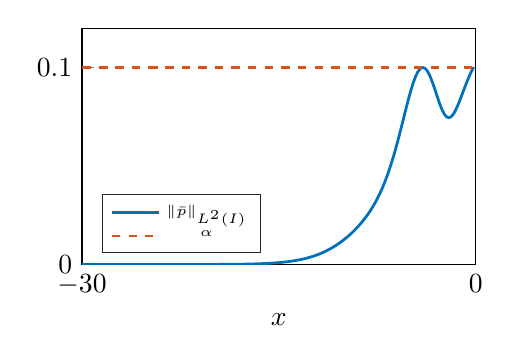
\begin{tikzpicture}

\begin{axis}[%
width=5cm,
height=3cm,
at={(0.0in,0.0in)},
scale only axis,
xmin=-30,
xmax=0,
xlabel={$x$},
xtick={-30,0},
ymin=0,
ymax=0.12,
ytick={0,0.1},
legend style={at={(0.05,0.05)},anchor=south west,draw=white!15!black}
]
\addplot [color=mycolor1,solid,line width=1.0pt]
  table[row sep=crcr]{%
-30	0\\
-29.999435258478	1.92001866238284e-09\\
-29.9977410551743	4.51428704488779e-09\\
-29.9949174538747	7.642257711991e-09\\
-29.9909645608861	1.11977572315335e-08\\
-29.9858825250328	1.51071279170889e-08\\
-29.9796715376505	1.93154009129659e-08\\
-29.9723318325794	2.37787692768681e-08\\
-29.9638636861552	2.84653124189212e-08\\
-29.9542674171988	3.33397752892541e-08\\
-29.9435433870045	3.83933155087214e-08\\
-29.9316919993258	4.35805494371696e-08\\
-29.9187137003607	4.89301511580612e-08\\
-29.904608978735	5.43630397159813e-08\\
-29.8893783654833	5.99680625980851e-08\\
-29.8730224340298	6.56066625746263e-08\\
-29.8555418001659	7.14521069338421e-08\\
-29.8369371220277	7.72829275472857e-08\\
-29.8172091000707	8.33781083247379e-08\\
-29.7963584770438	8.94150867697571e-08\\
-29.7743860379613	9.57937861364673e-08\\
-29.751292610073	1.02080729426765e-07\\
-29.7270790628334	1.08802464507461e-07\\
-29.7017463078689	1.15415106057011e-07\\
-29.6752952989434	1.22568585001686e-07\\
-29.6477270319225	1.29614671489487e-07\\
-29.6190425447357	1.37322354503618e-07\\
-29.589242917338	1.44940801757817e-07\\
-29.5583292716682	1.53361190114882e-07\\
-29.5263027716079	1.61722216275942e-07\\
-29.4931646229365	1.71046536702839e-07\\
-29.4589160732867	1.80353639235431e-07\\
-29.4235584120969	1.90796519204295e-07\\
-29.3870929705632	2.0128648165372e-07\\
-29.3495211215888	2.13076823570102e-07\\
-29.3108442797326	2.25010065872695e-07\\
-29.2710639011559	2.38388109227454e-07\\
-29.2301814835673	2.52029591640772e-07\\
-29.1881985661668	2.67244927125589e-07\\
-29.1451167295876	2.82848012453532e-07\\
-29.1009375958363	3.00146986223053e-07\\
-29.0556628282325	3.17949910462907e-07\\
-29.0092941313456	3.37554454654539e-07\\
-28.9618332509307	3.57778098754422e-07\\
-28.9132819738632	3.79875466747949e-07\\
-28.8636421280712	4.0270727094096e-07\\
-28.812915582467	4.27453280685347e-07\\
-28.7611042468761	4.53030988488106e-07\\
-28.7082100719663	4.80543685062865e-07\\
-28.6542350491731	5.08956824073613e-07\\
-28.5991812106258	5.39298961075322e-07\\
-28.5430506290703	5.70589682360172e-07\\
-28.4858454177911	6.03765657874259e-07\\
-28.4275677305322	6.37913409186787e-07\\
-28.3682197614156	6.73872644846043e-07\\
-28.3078037448588	7.10788142823932e-07\\
-28.2463219554906	7.49412270363534e-07\\
-28.1837767080657	7.88941292257282e-07\\
-28.1201703573772	8.30037274118704e-07\\
-28.0555052981684	8.71950311300533e-07\\
-27.9897839650422	9.15253615422708e-07\\
-27.9230088323695	9.59241301854187e-07\\
-27.8551824141965	1.00440703917653e-06\\
-27.7863072641493	1.05008361122049e-06\\
-27.7163859753386	1.09668597099703e-06\\
-27.6454211802613	1.14358304484402e-06\\
-27.5734155507017	1.19111882485101e-06\\
-27.5003717976313	1.23869080021761e-06\\
-27.4262926711059	1.2865775270786e-06\\
-27.3511809601629	1.3342057814852e-06\\
-27.2750394927157	1.38179324762892e-06\\
-27.1978711354475	1.42879175940935e-06\\
-27.1196787937033	1.47536807707734e-06\\
-27.0404654113807	1.52100028782154e-06\\
-26.9602339708186	1.56580784662061e-06\\
-26.8789874926856	1.60929787431147e-06\\
-26.7967290358655	1.65155411778677e-06\\
-26.7134616973427	1.6921142254427e-06\\
-26.6291886120856	1.7310335498227e-06\\
-26.5439129529281	1.76788952611739e-06\\
-26.4576379304506	1.80272037528164e-06\\
-26.370366792859	1.83514927606949e-06\\
-26.2821028258622	1.86521006913441e-06\\
-26.1928493525487	1.89258545768296e-06\\
-26.1026097332613	1.91731824459676e-06\\
-26.0113873654708	1.93916502368505e-06\\
-25.9191856836476	1.95819460348339e-06\\
-25.826008159133	1.97425696131564e-06\\
-25.7318583000082	1.98746627932614e-06\\
-25.636739650962	1.99779008471415e-06\\
-25.540655793158	2.00540832030391e-06\\
-25.4436103440989	2.01043440260774e-06\\
-25.3456069574912	2.0131401902e-06\\
-25.246649323107	2.01381696440422e-06\\
-25.1467411666451	2.01284908646606e-06\\
-25.0458862495914	2.01073947906805e-06\\
-24.9440883690764	2.00800721225575e-06\\
-24.8413513577327	2.00539170911445e-06\\
-24.7376790835508	2.00354722655748e-06\\
-24.6330754497331	2.00345907500231e-06\\
-24.5275443945475	2.00589494844294e-06\\
-24.4210898911785	2.01205516324654e-06\\
-24.3137159475778	2.0227489877622e-06\\
-24.205426606314	2.03931622893633e-06\\
-24.0962259444193	2.0624947596455e-06\\
-23.9861180732372	2.0936441082398e-06\\
-23.8751071382665	2.13329814394454e-06\\
-23.7631973190064	2.18272487391309e-06\\
-23.6503928287982	2.24217259257108e-06\\
-23.5366979146673	2.31278065071969e-06\\
-23.4221168571628	2.39454956599552e-06\\
-23.306653970197	2.48858701964843e-06\\
-23.1903136008821	2.5948366537998e-06\\
-23.0731001293674	2.71461173908735e-06\\
-22.9550179686738	2.84813062782986e-06\\
-22.8360715645278	2.99726596317506e-06\\
-22.7162653951945	3.16294703074812e-06\\
-22.5956039713084	3.34804030474933e-06\\
-22.4740918357038	3.55469220993082e-06\\
-22.351733563244	3.78723782280428e-06\\
-22.2285337606488	4.04956013800973e-06\\
-22.1044970663211	4.34790386566707e-06\\
-21.9796281501724	4.68832811321141e-06\\
-21.8539317134468	5.07929183474872e-06\\
-21.727412488544	5.52928823902012e-06\\
-21.6000752388414	6.04909330192662e-06\\
-21.4719247585146	6.64969826090319e-06\\
-21.3429658723565	7.34416697901059e-06\\
-21.2132034355964	8.14599735251774e-06\\
-21.0826423337168	9.07058155594966e-06\\
-20.9512874822692	1.01340918692402e-05\\
-20.8191438266896	1.1354548684807e-05\\
-20.686216342112	1.27512582579597e-05\\
-20.552510033181	1.4345489710737e-05\\
-20.4180299338636	1.61604368100197e-05\\
-20.2827811072595	1.82215135895305e-05\\
-20.1467686454106	2.05567928587957e-05\\
-20.0099976691091	2.31969458788705e-05\\
-19.8724733277052	2.61761179107812e-05\\
-19.7342007989124	2.95315470466894e-05\\
-19.5951852886133	3.3304851615074e-05\\
-19.4554320306634	3.75413651399153e-05\\
-19.3149462866937	4.22918241657552e-05\\
-19.1737333459133	4.761144978167e-05\\
-19.0317985249094	5.35620382546225e-05\\
-18.8891471674478	6.02108092507252e-05\\
-18.7457846442716	6.76329121063964e-05\\
-18.6017163528987	7.59100528775711e-05\\
-18.4569477174188	8.51334350108235e-05\\
-18.3114841882893	9.54021702909809e-05\\
-18.1653312421298	0.00010682667742484\\
-18.0184943815161	0.000119526874664724\\
-17.870979134773	0.000133636061960057\\
-17.7227910557662	0.00014929888869962\\
-17.5739357236932	0.000166675743486899\\
-17.4244187428729	0.000185940488621401\\
-17.2742457425354	0.000207285380084258\\
-17.123422376609	0.000230918559509963\\
-16.9719543235084	0.000257069526588343\\
-16.8198472859201	0.000285986383102749\\
-16.6671069905881	0.000317941878853318\\
-16.5137391880981	0.000353230413619445\\
-16.3597496526614	0.000392174677782692\\
-16.2051441818968	0.000435122435534339\\
-16.0499285966129	0.000482453783929824\\
-15.8941087405888	0.000534577764926411\\
-15.7376904803541	0.000591940267431815\\
-15.5806797049677	0.000655020546201119\\
-15.4230823257966	0.000724339785712332\\
-15.2649042762932	0.000800457631389638\\
-15.1061515117715	0.000883981415624817\\
-14.9468300091834	0.000975562816028398\\
-14.7869457668935	0.00107590769561288\\
-14.6265048044531	0.00118577297518374\\
-14.4655131623737	0.00130597693430524\\
-14.3039769018997	0.00143739629238725\\
-14.1419021047799	0.00158097662410956\\
-13.979294873039	0.00173772945295871\\
-13.8161613287472	0.00190874212805932\\
-13.6525076137903	0.00209517443190959\\
-13.4883398896382	0.00229826684898841\\
-13.3236643371129	0.0025193358192783\\
-13.1584871561558	0.00275977889768638\\
-12.9928145655946	0.00302106749082416\\
-12.8266528029085	0.0033047471972087\\
-12.660008123994	0.00361242691592044\\
-12.4928868029291	0.00394577302350139\\
-12.3252951317371	0.00430649445474807\\
-12.1572394201497	0.00469633062495433\\
-11.9887259953694	0.00511703358935937\\
-11.8197612018314	0.00557035178022276\\
-11.6503514009648	0.00605801238846062\\
-11.4805029709527	0.00658170562041007\\
-11.3102223064925	0.00714307237314584\\
-11.1395158185551	0.00774369607754398\\
-10.9683899341432	0.00838510189447419\\
-10.7968510960496	0.00906876464608359\\
-10.6249057626147	0.0097961258774203\\
-10.452560407483	0.0105686266839624\\
-10.2798215193598	0.0113877483383625\\
-10.1066956017666	0.0122550782675911\\
-9.93318917279629	0.0131723790029969\\
-9.75930876486789	0.0141416945794565\\
-9.58506092448047	0.0151654513467102\\
-9.41045221196674	0.0162466107520042\\
-9.23548920124605	0.0173888029641009\\
-9.06017847957684	0.0185965294044494\\
-8.88452664730872	0.0198753235822484\\
-8.70854031763387	0.0212319998651363\\
-8.53222611633815	0.022674821038657\\
-8.35559068155159	0.0242137726472798\\
-8.17864066349847	0.0258606876426495\\
-8.00138272424695	0.0276294892455423\\
-7.82382353745826	0.0295361735485601\\
-7.64596978813544	0.0315988997151513\\
-7.4678281723716	0.0338376598865641\\
-7.28940539709792	0.0362740043475304\\
-7.11070817983102	0.0389301462248223\\
-6.93174324842013	0.0418280156692247\\
-6.75251734079378	0.0449874930598345\\
-6.57303720470609	0.0484244569115632\\
-6.39330959748274	0.0521478982355987\\
-6.21334128576655	0.0561567920900691\\
-6.03313904526275	0.0604361768773082\\
-5.85270966048385	0.064953247316526\\
-5.67205992449419	0.0696533123610746\\
-5.49119663865423	0.0744566680616176\\
-5.31012661236446	0.0792567330420482\\
-5.12885666280904	0.0839207383095777\\
-4.9473936146991	0.0882934991428647\\
-4.76574430001584	0.0922052803796667\\
-4.5839155577533	0.0954835016233359\\
-4.40191423366085	0.0979679893844524\\
-4.21974717998547	0.099527790175258\\
-4.03742125521378	0.100077648538438\\
-3.85494332381379	0.0995911419472324\\
-3.67232025597648	0.0981088705769625\\
-3.48955892735714	0.095741026680053\\
-3.30666621881649	0.0926654533382166\\
-3.12364901616164	0.0891209162197756\\
-2.94051420988682	0.0853952476562407\\
-2.75726869491398	0.0818068187417183\\
-2.57391937033319	0.0786775520374651\\
-2.3904731391429	0.0762967643928936\\
-2.20693690799002	0.0748798693559522\\
-2.02331758690992	0.0745331613989123\\
-1.83962208906626	0.0752396210312267\\
-1.6558573304907	0.0768736194407294\\
-1.47203022982254	0.0792382042897569\\
-1.28814770804823	0.082108212832987\\
-1.10421668824077	0.0852654402013723\\
-0.920244095299094	0.0885198771189917\\
-0.736236855687364	0.0917194362800933\\
-0.552201897174141	0.0947517982896406\\
-0.368146148571595	0.0975428243279222\\
-0.184076539474632	0.100055125464602\\
};
\addlegendentry{\tiny $\|\bar p\|_{L^2(I)}$};

\addplot [color=mycolor2,dashed,line width=1.0pt]
  table[row sep=crcr]{%
-30	0.1\\
-29.999435258478	0.1\\
-29.9977410551743	0.1\\
-29.9949174538747	0.1\\
-29.9909645608861	0.1\\
-29.9858825250328	0.1\\
-29.9796715376505	0.1\\
-29.9723318325794	0.1\\
-29.9638636861552	0.1\\
-29.9542674171988	0.1\\
-29.9435433870045	0.1\\
-29.9316919993258	0.1\\
-29.9187137003607	0.1\\
-29.904608978735	0.1\\
-29.8893783654833	0.1\\
-29.8730224340298	0.1\\
-29.8555418001659	0.1\\
-29.8369371220277	0.1\\
-29.8172091000707	0.1\\
-29.7963584770438	0.1\\
-29.7743860379613	0.1\\
-29.751292610073	0.1\\
-29.7270790628334	0.1\\
-29.7017463078689	0.1\\
-29.6752952989434	0.1\\
-29.6477270319225	0.1\\
-29.6190425447357	0.1\\
-29.589242917338	0.1\\
-29.5583292716682	0.1\\
-29.5263027716079	0.1\\
-29.4931646229365	0.1\\
-29.4589160732867	0.1\\
-29.4235584120969	0.1\\
-29.3870929705632	0.1\\
-29.3495211215888	0.1\\
-29.3108442797326	0.1\\
-29.2710639011559	0.1\\
-29.2301814835673	0.1\\
-29.1881985661668	0.1\\
-29.1451167295876	0.1\\
-29.1009375958363	0.1\\
-29.0556628282325	0.1\\
-29.0092941313456	0.1\\
-28.9618332509307	0.1\\
-28.9132819738632	0.1\\
-28.8636421280712	0.1\\
-28.812915582467	0.1\\
-28.7611042468761	0.1\\
-28.7082100719663	0.1\\
-28.6542350491731	0.1\\
-28.5991812106258	0.1\\
-28.5430506290703	0.1\\
-28.4858454177911	0.1\\
-28.4275677305322	0.1\\
-28.3682197614156	0.1\\
-28.3078037448588	0.1\\
-28.2463219554906	0.1\\
-28.1837767080657	0.1\\
-28.1201703573772	0.1\\
-28.0555052981684	0.1\\
-27.9897839650422	0.1\\
-27.9230088323695	0.1\\
-27.8551824141965	0.1\\
-27.7863072641493	0.1\\
-27.7163859753386	0.1\\
-27.6454211802613	0.1\\
-27.5734155507017	0.1\\
-27.5003717976313	0.1\\
-27.4262926711059	0.1\\
-27.3511809601629	0.1\\
-27.2750394927157	0.1\\
-27.1978711354475	0.1\\
-27.1196787937033	0.1\\
-27.0404654113807	0.1\\
-26.9602339708186	0.1\\
-26.8789874926856	0.1\\
-26.7967290358655	0.1\\
-26.7134616973427	0.1\\
-26.6291886120856	0.1\\
-26.5439129529281	0.1\\
-26.4576379304506	0.1\\
-26.370366792859	0.1\\
-26.2821028258622	0.1\\
-26.1928493525487	0.1\\
-26.1026097332613	0.1\\
-26.0113873654708	0.1\\
-25.9191856836476	0.1\\
-25.826008159133	0.1\\
-25.7318583000082	0.1\\
-25.636739650962	0.1\\
-25.540655793158	0.1\\
-25.4436103440989	0.1\\
-25.3456069574912	0.1\\
-25.246649323107	0.1\\
-25.1467411666451	0.1\\
-25.0458862495914	0.1\\
-24.9440883690764	0.1\\
-24.8413513577327	0.1\\
-24.7376790835508	0.1\\
-24.6330754497331	0.1\\
-24.5275443945475	0.1\\
-24.4210898911785	0.1\\
-24.3137159475778	0.1\\
-24.205426606314	0.1\\
-24.0962259444193	0.1\\
-23.9861180732372	0.1\\
-23.8751071382665	0.1\\
-23.7631973190064	0.1\\
-23.6503928287982	0.1\\
-23.5366979146673	0.1\\
-23.4221168571628	0.1\\
-23.306653970197	0.1\\
-23.1903136008821	0.1\\
-23.0731001293674	0.1\\
-22.9550179686738	0.1\\
-22.8360715645278	0.1\\
-22.7162653951945	0.1\\
-22.5956039713084	0.1\\
-22.4740918357038	0.1\\
-22.351733563244	0.1\\
-22.2285337606488	0.1\\
-22.1044970663211	0.1\\
-21.9796281501724	0.1\\
-21.8539317134468	0.1\\
-21.727412488544	0.1\\
-21.6000752388414	0.1\\
-21.4719247585146	0.1\\
-21.3429658723565	0.1\\
-21.2132034355964	0.1\\
-21.0826423337168	0.1\\
-20.9512874822692	0.1\\
-20.8191438266896	0.1\\
-20.686216342112	0.1\\
-20.552510033181	0.1\\
-20.4180299338636	0.1\\
-20.2827811072595	0.1\\
-20.1467686454106	0.1\\
-20.0099976691091	0.1\\
-19.8724733277052	0.1\\
-19.7342007989124	0.1\\
-19.5951852886133	0.1\\
-19.4554320306634	0.1\\
-19.3149462866937	0.1\\
-19.1737333459133	0.1\\
-19.0317985249094	0.1\\
-18.8891471674478	0.1\\
-18.7457846442716	0.1\\
-18.6017163528987	0.1\\
-18.4569477174188	0.1\\
-18.3114841882893	0.1\\
-18.1653312421298	0.1\\
-18.0184943815161	0.1\\
-17.870979134773	0.1\\
-17.7227910557662	0.1\\
-17.5739357236932	0.1\\
-17.4244187428729	0.1\\
-17.2742457425354	0.1\\
-17.123422376609	0.1\\
-16.9719543235084	0.1\\
-16.8198472859201	0.1\\
-16.6671069905881	0.1\\
-16.5137391880981	0.1\\
-16.3597496526614	0.1\\
-16.2051441818968	0.1\\
-16.0499285966129	0.1\\
-15.8941087405888	0.1\\
-15.7376904803541	0.1\\
-15.5806797049677	0.1\\
-15.4230823257966	0.1\\
-15.2649042762932	0.1\\
-15.1061515117715	0.1\\
-14.9468300091834	0.1\\
-14.7869457668935	0.1\\
-14.6265048044531	0.1\\
-14.4655131623737	0.1\\
-14.3039769018997	0.1\\
-14.1419021047799	0.1\\
-13.979294873039	0.1\\
-13.8161613287472	0.1\\
-13.6525076137903	0.1\\
-13.4883398896382	0.1\\
-13.3236643371129	0.1\\
-13.1584871561558	0.1\\
-12.9928145655946	0.1\\
-12.8266528029085	0.1\\
-12.660008123994	0.1\\
-12.4928868029291	0.1\\
-12.3252951317371	0.1\\
-12.1572394201497	0.1\\
-11.9887259953694	0.1\\
-11.8197612018314	0.1\\
-11.6503514009648	0.1\\
-11.4805029709527	0.1\\
-11.3102223064925	0.1\\
-11.1395158185551	0.1\\
-10.9683899341432	0.1\\
-10.7968510960496	0.1\\
-10.6249057626147	0.1\\
-10.452560407483	0.1\\
-10.2798215193598	0.1\\
-10.1066956017666	0.1\\
-9.93318917279629	0.1\\
-9.75930876486789	0.1\\
-9.58506092448047	0.1\\
-9.41045221196674	0.1\\
-9.23548920124605	0.1\\
-9.06017847957684	0.1\\
-8.88452664730872	0.1\\
-8.70854031763387	0.1\\
-8.53222611633815	0.1\\
-8.35559068155159	0.1\\
-8.17864066349847	0.1\\
-8.00138272424695	0.1\\
-7.82382353745826	0.1\\
-7.64596978813544	0.1\\
-7.4678281723716	0.1\\
-7.28940539709792	0.1\\
-7.11070817983102	0.1\\
-6.93174324842013	0.1\\
-6.75251734079378	0.1\\
-6.57303720470609	0.1\\
-6.39330959748274	0.1\\
-6.21334128576655	0.1\\
-6.03313904526275	0.1\\
-5.85270966048385	0.1\\
-5.67205992449419	0.1\\
-5.49119663865423	0.1\\
-5.31012661236446	0.1\\
-5.12885666280904	0.1\\
-4.9473936146991	0.1\\
-4.76574430001584	0.1\\
-4.5839155577533	0.1\\
-4.40191423366085	0.1\\
-4.21974717998547	0.1\\
-4.03742125521378	0.1\\
-3.85494332381379	0.1\\
-3.67232025597648	0.1\\
-3.48955892735714	0.1\\
-3.30666621881649	0.1\\
-3.12364901616164	0.1\\
-2.94051420988682	0.1\\
-2.75726869491398	0.1\\
-2.57391937033319	0.1\\
-2.3904731391429	0.1\\
-2.20693690799002	0.1\\
-2.02331758690992	0.1\\
-1.83962208906626	0.1\\
-1.6558573304907	0.1\\
-1.47203022982254	0.1\\
-1.28814770804823	0.1\\
-1.10421668824077	0.1\\
-0.920244095299094	0.1\\
-0.736236855687364	0.1\\
-0.552201897174141	0.1\\
-0.368146148571595	0.1\\
-0.184076539474632	0.1\\
};
\addlegendentry{\tiny $\alpha$};

\end{axis}
\end{tikzpicture}% 
\caption{Spatial support of the control determined by $\|\bar p(x)\|_{L^2(I)}=\alpha$.}
\label{supportIP}
\end{figure}
We clearly see that the support of the optimal control correlates with the spatial positions where $\|\bar p(x)\|_{L^2(I)}=\alpha$ holds. The optimal state $\bar y$ is shown in \cref{ex2fullgammadm5}. An upstream soliton is created that matches accurately the objective wave $z$ at terminal time. Naturally, spurious waves are created on the control domain which have no contribution to the cost functional.
\begin{figure}[htb]
\centering
\subfloat{% This file was created by matlab2tikz.
% Minimal pgfplots version: 1.3
%
%The latest updates can be retrieved from
%  http://www.mathworks.com/matlabcentral/fileexchange/22022-matlab2tikz
%where you can also make suggestions and rate matlab2tikz.
%
\begin{tikzpicture}

\begin{axis}[%
width=5cm,
height=3cm,
at={(0.0in,0.0in)},
scale only axis,
axis on top,
xmin=-0.00499750124937531,
xmax=20.0049975012494,
xlabel={$t$},
ymin=-30.05859375,
ymax=30.05859375,
ylabel={$x$},
colormap={mymap}{[1pt] rgb(0pt)=(0.2081,0.1663,0.5292); rgb(1pt)=(0.211624,0.189781,0.577676); rgb(2pt)=(0.212252,0.213771,0.626971); rgb(3pt)=(0.2081,0.2386,0.677086); rgb(4pt)=(0.195905,0.264457,0.7279); rgb(5pt)=(0.170729,0.291938,0.779248); rgb(6pt)=(0.125271,0.324243,0.830271); rgb(7pt)=(0.0591333,0.359833,0.868333); rgb(8pt)=(0.0116952,0.38751,0.881957); rgb(9pt)=(0.00595714,0.408614,0.882843); rgb(10pt)=(0.0165143,0.4266,0.878633); rgb(11pt)=(0.0328524,0.443043,0.871957); rgb(12pt)=(0.0498143,0.458571,0.864057); rgb(13pt)=(0.0629333,0.47369,0.855438); rgb(14pt)=(0.0722667,0.488667,0.8467); rgb(15pt)=(0.0779429,0.503986,0.838371); rgb(16pt)=(0.0793476,0.520024,0.831181); rgb(17pt)=(0.0749429,0.537543,0.826271); rgb(18pt)=(0.0640571,0.556986,0.823957); rgb(19pt)=(0.0487714,0.577224,0.822829); rgb(20pt)=(0.0343429,0.596581,0.819852); rgb(21pt)=(0.0265,0.6137,0.8135); rgb(22pt)=(0.0238905,0.628662,0.803762); rgb(23pt)=(0.0230905,0.641786,0.791267); rgb(24pt)=(0.0227714,0.653486,0.776757); rgb(25pt)=(0.0266619,0.664195,0.760719); rgb(26pt)=(0.0383714,0.674271,0.743552); rgb(27pt)=(0.0589714,0.683757,0.725386); rgb(28pt)=(0.0843,0.692833,0.706167); rgb(29pt)=(0.113295,0.7015,0.685857); rgb(30pt)=(0.145271,0.709757,0.664629); rgb(31pt)=(0.180133,0.717657,0.642433); rgb(32pt)=(0.217829,0.725043,0.619262); rgb(33pt)=(0.258643,0.731714,0.595429); rgb(34pt)=(0.302171,0.737605,0.571186); rgb(35pt)=(0.348167,0.742433,0.547267); rgb(36pt)=(0.395257,0.7459,0.524443); rgb(37pt)=(0.44201,0.748081,0.503314); rgb(38pt)=(0.487124,0.749062,0.483976); rgb(39pt)=(0.530029,0.749114,0.466114); rgb(40pt)=(0.570857,0.748519,0.44939); rgb(41pt)=(0.609852,0.747314,0.433686); rgb(42pt)=(0.6473,0.7456,0.4188); rgb(43pt)=(0.683419,0.743476,0.404433); rgb(44pt)=(0.71841,0.741133,0.390476); rgb(45pt)=(0.752486,0.7384,0.376814); rgb(46pt)=(0.785843,0.735567,0.363271); rgb(47pt)=(0.818505,0.732733,0.34979); rgb(48pt)=(0.850657,0.7299,0.336029); rgb(49pt)=(0.882433,0.727433,0.3217); rgb(50pt)=(0.913933,0.725786,0.306276); rgb(51pt)=(0.944957,0.726114,0.288643); rgb(52pt)=(0.973895,0.731395,0.266648); rgb(53pt)=(0.993771,0.745457,0.240348); rgb(54pt)=(0.999043,0.765314,0.216414); rgb(55pt)=(0.995533,0.786057,0.196652); rgb(56pt)=(0.988,0.8066,0.179367); rgb(57pt)=(0.978857,0.827143,0.163314); rgb(58pt)=(0.9697,0.848138,0.147452); rgb(59pt)=(0.962586,0.870514,0.1309); rgb(60pt)=(0.958871,0.8949,0.113243); rgb(61pt)=(0.959824,0.921833,0.0948381); rgb(62pt)=(0.9661,0.951443,0.0755333); rgb(63pt)=(0.9763,0.9831,0.0538)},
colorbar horizontal,
colorbar style={at={(0.5,1.03)},anchor=south,xticklabel pos=upper},
point meta min=-0.627562291261057,
point meta max=1.3988340293968
]
\addplot [forget plot] graphics [xmin=-0.00499750124937531,xmax=20.0049975012494,ymin=-30.05859375,ymax=30.05859375] {images/state-1.png};
\end{axis}
\end{tikzpicture}% }\quad
\subfloat{% This file was created by matlab2tikz.
% Minimal pgfplots version: 1.3
%
%The latest updates can be retrieved from
%  http://www.mathworks.com/matlabcentral/fileexchange/22022-matlab2tikz
%where you can also make suggestions and rate matlab2tikz.
%
\definecolor{mycolor1}{rgb}{0.00000,0.44700,0.74100}%
\definecolor{mycolor2}{rgb}{0.85000,0.32500,0.09800}%
%
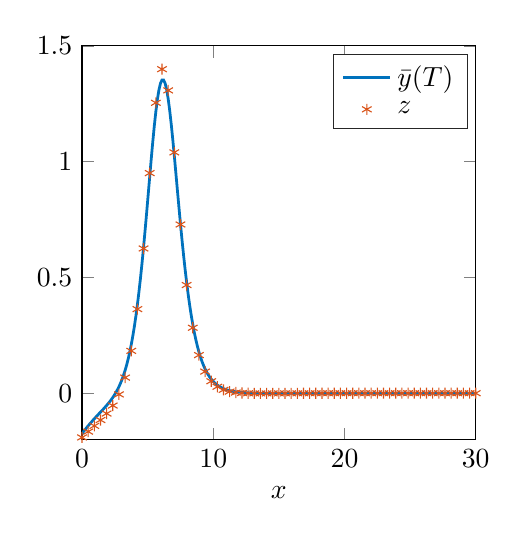
\begin{tikzpicture}

\begin{axis}[%
width=5cm,
height=5cm,
at={(0.0in,0.0in)},
scale only axis,
xmin=0,
xmax=30,
xlabel={$x$},
ymin=-0.2,
ymax=1.5,
legend style={legend cell align=left,align=left,draw=white!15!black}
]
\addplot [color=mycolor1,solid,line width = 1pt]
  table[row sep=crcr]{%
0	-0.175906727462304\\
0.1171875	-0.165300349105138\\
0.234375	-0.157883539219922\\
0.3515625	-0.148602156396641\\
0.46875	-0.141279067062128\\
0.5859375	-0.132689574644709\\
0.703125	-0.125575696503086\\
0.8203125	-0.117518719242859\\
0.9375	-0.110620842795291\\
1.0546875	-0.102956727062682\\
1.171875	-0.0962044014917816\\
1.2890625	-0.088775407687326\\
1.40625	-0.0820408733122654\\
1.5234375	-0.0746560983564858\\
1.640625	-0.0677562411692003\\
1.7578125	-0.0601786885151956\\
1.875	-0.0528682267393792\\
1.9921875	-0.0448000304160034\\
2.109375	-0.036758671463504\\
2.2265625	-0.0278230799360569\\
2.34375	-0.0186375938563029\\
2.4609375	-0.00835727941103772\\
2.578125	0.00250075747598086\\
2.6953125	0.0147285409184496\\
2.8125	0.0279277788820869\\
2.9296875	0.0428570846651206\\
3.046875	0.0592307325393429\\
3.1640625	0.0777889913999125\\
3.28125	0.0983514709399749\\
3.3984375	0.121648316272313\\
3.515625	0.147591620072356\\
3.6328125	0.176898140839259\\
3.75	0.209547181404277\\
3.8671875	0.246220120626087\\
3.984375	0.286916631477777\\
4.1015625	0.332232586172607\\
4.21875	0.382109395395346\\
4.3359375	0.436970208282862\\
4.453125	0.496580773405434\\
4.5703125	0.561065241113834\\
4.6875	0.629862820687575\\
4.8046875	0.702649747386886\\
4.921875	0.77838497784549\\
5.0390625	0.856173098569013\\
5.15625	0.934402323315562\\
5.2734375	1.01158912493888\\
5.390625	1.08561584427908\\
5.5078125	1.15459161362533\\
5.625	1.21618512933884\\
5.7421875	1.26850958854118\\
5.859375	1.30951650729586\\
5.9765625	1.33787168494385\\
6.09375	1.35234613082245\\
6.2109375	1.35262327361262\\
6.328125	1.33862412166363\\
6.4453125	1.31120078342299\\
6.5625	1.27137709339049\\
6.6796875	1.22093360485098\\
6.796875	1.16160329850933\\
6.9140625	1.09559746117484\\
7.03125	1.02482456411173\\
7.1484375	0.951411575913236\\
7.265625	0.876998432128768\\
7.3828125	0.803281282355517\\
7.5	0.731398262058778\\
7.6171875	0.66248922904654\\
7.734375	0.597159993504345\\
7.8515625	0.53603737685281\\
7.96875	0.479289461670427\\
8.0859375	0.427155761457185\\
8.203125	0.379504785085131\\
8.3203125	0.336327616953374\\
8.4375	0.297321844241092\\
8.5546875	0.262345199808551\\
8.671875	0.231021150090672\\
8.7890625	0.203154440927353\\
8.90625	0.178357040751831\\
9.0234375	0.156429603875433\\
9.140625	0.137007687898864\\
9.2578125	0.119913471941984\\
9.375	0.104822254271934\\
9.4921875	0.0915882631713771\\
9.609375	0.0799311242970285\\
9.7265625	0.0697388890141378\\
9.84375	0.0607738118188909\\
9.9609375	0.0529550671992389\\
10.078125	0.0460829283671865\\
10.1953125	0.0401031301218258\\
10.3125	0.0348484076456787\\
10.4296875	0.0302860865058701\\
10.546875	0.0262758990698695\\
10.6640625	0.0228021140372675\\
10.78125	0.0197465663781417\\
10.8984375	0.0171064462706962\\
11.015625	0.0147815302796745\\
11.1328125	0.0127786086884953\\
11.25	0.0110119729208328\\
11.3671875	0.0094953534716976\\
11.484375	0.00815479067455218\\
11.6015625	0.00700887104440842\\
11.71875	0.00599317916010131\\
11.8359375	0.00512955128898588\\
11.953125	0.00436137212995298\\
12.0703125	0.00371250624933436\\
12.1875	0.0031327640182847\\
12.3046875	0.00264712054045535\\
12.421875	0.00221072967585826\\
12.5390625	0.00184899565059523\\
12.65625	0.0015215626675284\\
12.7734375	0.00125376441222589\\
12.890625	0.00100906077076389\\
13.0078125	0.000812354114146506\\
13.125	0.000630383652145749\\
13.2421875	0.000487365119224178\\
13.359375	0.000352888061520758\\
13.4765625	0.000250305530302025\\
13.59375	0.000151711655380095\\
13.7109375	7.94805481721109e-05\\
13.828125	7.92946241222157e-06\\
13.9453125	-4.16181577982165e-05\\
14.0625	-9.28529557242095e-05\\
14.1796875	-0.00012554109262452\\
14.296875	-0.000161573062112066\\
14.4140625	-0.000181818894704433\\
14.53125	-0.000206530361449869\\
14.6484375	-0.000217678139039755\\
14.765625	-0.000234012116770468\\
14.8828125	-0.000238587593563419\\
15	-0.000248770721400007\\
15.1171875	-0.000248675944681567\\
15.234375	-0.00025438828181059\\
15.3515625	-0.000251050144917136\\
15.46875	-0.000253555589969236\\
15.5859375	-0.000248039015255614\\
15.703125	-0.000248284316822069\\
15.8203125	-0.000241379462680333\\
15.9375	-0.0002400700306873\\
16.0546875	-0.000232357904374638\\
16.171875	-0.000230016193042135\\
16.2890625	-0.000221919548487251\\
16.40625	-0.000218928590547738\\
16.5234375	-0.000210750578336502\\
16.640625	-0.00020738853922602\\
16.7578125	-0.000199341618968058\\
16.875	-0.000195807097578699\\
16.9921875	-0.000188036397706982\\
17.109375	-0.000184468162509082\\
17.2265625	-0.000177067650500381\\
17.34375	-0.000173560184517009\\
17.4609375	-0.000166586517361552\\
17.578125	-0.000163200554320585\\
17.6953125	-0.000156682721883802\\
17.8125	-0.000153455171035352\\
17.9296875	-0.000147401879728644\\
18.046875	-0.000144351399842363\\
18.1640625	-0.000138757601895183\\
18.28125	-0.000135890518437743\\
18.3984375	-0.000130740700791136\\
18.515625	-0.000128054504458261\\
18.6328125	-0.000123327321841803\\
18.75	-0.000120813494630536\\
18.8671875	-0.000116483021677049\\
18.984375	-0.000114129828540918\\
19.1015625	-0.000110168538735474\\
19.21875	-0.000107961752937715\\
19.3359375	-0.000104341110783059\\
19.453125	-0.000102266421608012\\
19.5703125	-9.89583945229407e-05\\
19.6875	-9.70009715745621e-05\\
19.8046875	-9.39785580093793e-05\\
19.921875	-9.21250495808621e-05\\
20.0390625	-8.93627095819859e-05\\
20.15625	-8.76002657831446e-05\\
20.2734375	-8.5074456299949e-05\\
20.390625	-8.33923495539108e-05\\
20.5078125	-8.10813602284848e-05\\
20.625	-7.94697426517451e-05\\
20.7421875	-7.73540709787453e-05\\
20.859375	-7.5805342622897e-05\\
20.9765625	-7.38674158144657e-05\\
21.09375	-7.2374837212191e-05\\
21.2109375	-7.05989849652904e-05\\
21.328125	-6.915784678976e-05\\
21.4453125	-6.75303117944085e-05\\
21.5625	-6.61366122195545e-05\\
21.6796875	-6.46449514684404e-05\\
21.796875	-6.32961893785202e-05\\
21.9140625	-6.19297295823477e-05\\
22.03125	-6.06240221701888e-05\\
22.1484375	-5.93728211253635e-05\\
22.265625	-5.81090034321016e-05\\
22.3828125	-5.69644338427129e-05\\
22.5	-5.57418281867132e-05\\
22.6171875	-5.46955490385758e-05\\
22.734375	-5.3513266916951e-05\\
22.8515625	-5.25572056504739e-05\\
22.96875	-5.14140362436075e-05\\
23.0859375	-5.05394845568039e-05\\
23.203125	-4.94325169413946e-05\\
23.3203125	-4.86288758501163e-05\\
23.4375	-4.75524033748143e-05\\
23.5546875	-4.68057643956221e-05\\
23.671875	-4.57493736331256e-05\\
23.7890625	-4.5040433900044e-05\\
23.90625	-4.39872054092047e-05\\
24.0234375	-4.32899173770668e-05\\
24.140625	-4.22155740313581e-05\\
24.2578125	-4.14969519989214e-05\\
24.375	-4.03706821136542e-05\\
24.4921875	-3.95929339837295e-05\\
24.609375	-3.83809351885876e-05\\
24.7265625	-3.75063105252602e-05\\
24.84375	-3.61777484354941e-05\\
24.9609375	-3.51753335312159e-05\\
25.078125	-3.37095944866136e-05\\
25.1953125	-3.25625144132302e-05\\
25.3125	-3.09557728108418e-05\\
25.4296875	-2.96665733008965e-05\\
25.546875	-2.79355256965269e-05\\
25.6640625	-2.65279487742654e-05\\
25.78125	-2.47094438258636e-05\\
25.8984375	-2.32259101944131e-05\\
26.015625	-2.13724206362557e-05\\
26.1328125	-1.98678189512244e-05\\
26.25	-1.80399571784603e-05\\
26.3671875	-1.65733991303325e-05\\
26.484375	-1.48314033646395e-05\\
26.6015625	-1.34579512906082e-05\\
26.71875	-1.18540701623202e-05\\
26.8359375	-1.06181463235875e-05\\
26.953125	-9.19130135803159e-06\\
27.0703125	-8.12275397948699e-06\\
27.1875	-6.89603407241229e-06\\
27.3046875	-6.00901894768501e-06\\
27.421875	-4.98982661855325e-06\\
27.5390625	-4.28404620655474e-06\\
27.65625	-3.46622879457627e-06\\
27.7734375	-2.92972537212649e-06\\
27.890625	-2.29682855944923e-06\\
28.0078125	-1.90947955830537e-06\\
28.125	-1.43833519527287e-06\\
28.2421875	-1.17536101191228e-06\\
28.359375	-8.39431800340147e-07\\
28.4765625	-6.74459506523229e-07\\
28.59375	-4.46599694073962e-07\\
28.7109375	-3.54058017935058e-07\\
28.828125	-2.08563812032836e-07\\
28.9453125	-1.65375934474454e-07\\
29.0625	-7.93553396917615e-08\\
29.1796875	-6.60194595787908e-08\\
29.296875	-2.01956000054565e-08\\
29.4140625	-2.14036778776442e-08\\
29.53125	-4.91173176598395e-10\\
29.6484375	-5.45834507765167e-09\\
29.765625	1.77012703105861e-09\\
29.8828125	-9.27796978687197e-10\\
30	0\\
};
\addlegendentry{$\bar y(T)$};

\addplot [color=mycolor2,only marks,mark=asterisk,mark options={solid}]
  table[row sep=crcr]{%
0	-0.19107600324811\\
0.46875	-0.165858954505256\\
0.9375	-0.141155367547741\\
1.40625	-0.115856214495644\\
1.875	-0.0878550670217143\\
2.34375	-0.0532938314873238\\
2.8125	-0.00534809514411409\\
3.28125	0.0674598795267957\\
3.75	0.182771668354493\\
4.21875	0.363057638505416\\
4.6875	0.624825032353612\\
5.15625	0.950432918374239\\
5.625	1.25396439421819\\
6.09375	1.39914426423522\\
6.5625	1.30751039934605\\
7.03125	1.03982782266806\\
7.5	0.728502655144989\\
7.96875	0.467069798990587\\
8.4375	0.28258068514618\\
8.90625	0.164605776294786\\
9.375	0.0933004144897742\\
9.84375	0.05160647415781\\
10.3125	0.027740023404666\\
10.78125	0.0143040473264534\\
11.25	0.00686928079451349\\
11.71875	0.00284730809641459\\
12.1875	0.000745302894166253\\
12.65625	-0.000290722734136554\\
13.125	-0.000746057751602231\\
13.59375	-0.000894369219002267\\
14.0625	-0.000888329883630556\\
14.53125	-0.000811728180256484\\
15	-0.000709367026910097\\
15.46875	-0.000604190328605039\\
15.9375	-0.000507061162927481\\
16.40625	-0.000422304154165534\\
16.875	-0.000350823659854815\\
17.34375	-0.000291841181839992\\
17.8125	-0.000243844310403547\\
18.28125	-0.000205093643976611\\
18.75	-0.000173888133336431\\
19.21875	-0.00014869692275174\\
19.6875	-0.000128215772700557\\
20.15625	-0.000111381012722735\\
20.625	-9.73592519219394e-05\\
21.09375	-8.55226012351301e-05\\
21.5625	-7.54155071513049e-05\\
22.03125	-6.67185092223435e-05\\
22.5	-5.9213542888263e-05\\
22.96875	-5.27484229092452e-05\\
23.4375	-4.7183834778993e-05\\
23.90625	-4.23120873518655e-05\\
24.375	-3.777325026437e-05\\
24.84375	-3.30418519429905e-05\\
25.3125	-2.76497855037129e-05\\
25.78125	-2.15569608902061e-05\\
26.25	-1.52718678349054e-05\\
26.71875	-9.59235105544111e-06\\
27.1875	-5.16105977229408e-06\\
27.65625	-2.21396636337168e-06\\
28.125	-5.93609825097644e-07\\
28.59375	7.17438565543935e-08\\
29.0625	1.91073924779312e-07\\
29.53125	9.5552421258141e-08\\
30	0\\
};
\addlegendentry{$z$};

\end{axis}
\end{tikzpicture}% }
\caption{Left: Evolution of the optimal state $\bar y$ for $\rg = 10^{-5}$, Right: Terminal state $\bar y(T)$ compared with $z$}
\label{ex2fullgammadm5}
\end{figure}




%%% Local Variables:
%%% mode: latex
%%% TeX-master: "kdv.tex"
%%% End: 